\documentclass[supercite]{Experimental_Report}
\title{~~~~~~C语言程序设计实验~~~~~~}
\author{阮云轩}
%\coauthor{张三、李四}
\school{计算机科学与技术学院}
\classnum{CS2404}
\stunum{U202490035}
%\costunum{U202115631、U202115631}
\instructor{卢萍} % 该系列实验报告模板由华科大计院教师陈加忠制作
\date{2024年11月22日}

\usepackage{algorithm, multirow}
\usepackage{algpseudocode}
\usepackage{amsmath}
\usepackage{amsthm}
\usepackage{framed}
\usepackage{mathtools}
\usepackage{subcaption}
\usepackage{xltxtra} %提供了针对XeTeX的改进并且加入了XeTeX的LOGO, 自动调用xunicode宏包(提供Unicode字符宏)
\usepackage{bm}
\usepackage{tikz}
\usepackage{tikzscale}
\usepackage{pgfplots}
\usepackage{listings}
\usepackage{tocloft}
%\usepackage{enumerate}
\lstdefinestyle{commonCodeStyle}{
	language = C, % 假设主要是C语言代码，可按需更改语言类型
	basicstyle=\ttfamily\footnotesize, % 设置字体为等宽且小一号字体，方便排版
	breaklines = true, % 自动换行
	breakatwhitespace = true, % 尽量在空白处换行
	columns=flexible, % 灵活调整列宽，让代码适应页面宽度
	numbers=left, % 在代码左侧显示行号
	numberstyle=\tiny\color{gray}, % 行号的样式，设置为小字号灰色字体
	keywordstyle=\color{blue}\bfseries, % 关键字样式，加粗蓝色显示
	commentstyle=\itshape, % 注释样式，斜体绿色显示
	stringstyle=\color{magenta}, % 字符串样式，紫红色显示
	showstringspaces=false % 取消显示字符串中的空格，放在正确位置
}

\lstdefinestyle{mycode}{
	language = C,
	basicstyle=\ttfamily,
	breaklines = true,
	breakatwhitespace = true,
	stringstyle=\ttfamily, % 设置字符串的字体风格保持和基本字体一致（等宽字体），这里也可以根据喜好设置其他样式，若不想设置额外样式可不写此行
	showstringspaces=false % 关键在于这一行，用于取消显示字符串中的空格
}
%\usepackage{enumerate}

\pgfplotsset{compat=1.16}

\newcommand{\cfig}[3]{
	\begin{figure}[htb]
		\centering
		\includegraphics[width=#2\textwidth]{images/#1.tikz}
		\caption{#3}
		\label{fig:#1}
	\end{figure}
}

\newcommand{\sfig}[3]{
	\begin{subfigure}[b]{#2\textwidth}
		\includegraphics[width=\textwidth]{images/#1.tikz}
		\caption{#3}
		\label{fig:#1}
	\end{subfigure}
}

\newcommand{\xfig}[3]{
	\begin{figure}[htb]
		\centering
		#3
		\caption{#2}
		\label{fig:#1}
	\end{figure}
}
\renewcommand{\cftlstlistingpresnum}{代码 }
\renewcommand{\cftlstlistingaftersnum}{:}
\setlength{\cftlstlistingnumwidth}{3.5em}

\newcommand{\rfig}[1]{\autoref{fig:#1}}
\newcommand{\ralg}[1]{\autoref{alg:#1}}
\newcommand{\rthm}[1]{\autoref{thm:#1}}
\newcommand{\rlem}[1]{\autoref{lem:#1}}
\newcommand{\reqn}[1]{\autoref{eqn:#1}}
\newcommand{\rtbl}[1]{\autoref{tbl:#1}}

\algnewcommand\Null{\textsc{null }}
\algnewcommand\algorithmicinput{\textbf{Input:}}
\algnewcommand\Input{\item[\algorithmicinput]}
\algnewcommand\algorithmicoutput{\textbf{Output:}}
\algnewcommand\Output{\item[\algorithmicoutput]}
\algnewcommand\algorithmicbreak{\textbf{break}}
\algnewcommand\Break{\algorithmicbreak}
\algnewcommand\algorithmiccontinue{\textbf{continue}}
\algnewcommand\Continue{\algorithmiccontinue}
\algnewcommand{\LeftCom}[1]{\State $\triangleright$ #1}

\newtheorem{thm}{定理}[section]
\newtheorem{lem}{引理}[section]

\makeatletter
% 定义 \subsubsubsection 命令
\newcommand{\subsubsubsection}{\@startsection{subsubsubsection}{4}{\z@}{-3.25ex plus -1ex minus -.2ex}{1.5ex plus.2ex}{\normalfont\Large\bfseries}}
% 定义 \subsubsubsubsection 命令
\newcommand{\subsubsubsubsection}{\@startsection{subsubsubsubsection}{5}{\z@}{-3.25ex plus -1ex minus -.2ex}{1.5ex plus.2ex}{\normalfont\large\bfseries}}
% 定义 \subsubsubsubsubsection 命令
\newcommand{\subsubsubsubsubsection}{\@startsection{subsubsubsubsubsection}{6}{\z@}{-3.25ex plus -1ex minus -.2ex}{1.5ex plus.2ex}{\normalfont\normalsize\bfseries}}
\makeatother

\colorlet{shadecolor}{black!15}

\theoremstyle{definition}
\newtheorem{alg}{算法}[section]

\def\thmautorefname~#1\null{定理~#1~\null}
\def\lemautorefname~#1\null{引理~#1~\null}
\def\algautorefname~#1\null{算法~#1~\null}

\begin{document}
	
	\maketitle
	
	\clearpage
	
	\pagenumbering{Roman}
	
	\tableofcontents[level=2]
	
	\clearpage
	
	\pagenumbering{arabic}
	
	\listoflistings
	\section{摘要}
	
	\subsection{關於行文}
	由於筆者習慣 以漢字(繁體中文)以行文，在實驗報告中，在杜撰時經己盡量轉換成 漢字(簡體中文)，但難免會有 漢字(繁體中文)的出現。還請讀者見諒。
	\subsection{前言}
	本C语言程序课程实验报告是由LateX编写的，主要写了关于数组和结构的实验题。本实验报告包括但不限于对实验题目的分析，提出对题目的理解和需要注意的相关事项，构建对应的设计思路，利用相关流程图去说明以便于和个人读者理解，给出相关报行代码供以读者自运行测试，还带有章节的小结点出相关的数据结构和编程思维，最后还有个人感俉指点对C语言的理解和个人收获。
	\\由于作者水平有限，难免有些缺点和错误，望广大读者给予批评指正。

\begin{lstlisting}[style=commonCodeStyle, caption={示例}, label={lst:0-0}]
	#include <stdio.h>
	int main() {
	printf("Hello, C!\n"); //print out Hello, C!
	return 0;
	}
\end{lstlisting}
以上是本實驗報告時頻繁出現的編程文本格式，示味着相關的說明部分(\ref{lst:0-0})
	
	\section{实验五 数组}
		\subsection{5-1 程序改错与跟踪调试}
		
		目標要求：\\
		在下面所给的源程序中,函数strncate(t,s)的功能是将字符串s连接到字符串t的尾部; 函数 strdele(s,c)的功能是从字符串s中删除所有与给定字符c相同的字符,程序应该能
		够输出如下结果(\ref{lst:5-1-1}):
\begin{lstlisting}[style=commonCodeStyle, caption={示例}, label={lst:5-1-1}]
	Programming Language
	ProgrammingLanguageLanguage 
	ProgrmmingLnguge
\end{lstlisting}
		跟踪和分析源程序中存在的问题,排除程序中的各种逻辑错误,使之能够输出正确结果。
		\subsubsection{相关修正补充}
		\subsubsubsection{目標程序}
		\begin{lstlisting}[style=commonCodeStyle, caption={目標程序}, label={lst:5-1-2}]
			/*实验5-1程序改错与跟踪调试题程序*/
			#include<stdio.h>
			void strcate (char [], char []);
			void strdelc (char [], char);
			int main (void)
			{
				char a[ ]="Language", b[ ]="Programming"; //問題一
				printf("%s %s\n",b,a);
				strcate (b, a); printf("%s %s\n",b,a);
				strdelc(b, 'a'); printf("%s\n",b);
				return 0;
			}
			void strcate(char t[ ], char s[])
			{
				int i=0,j=0;
				while(t[i++]); //問題二
				while((t[i++] = s[j++])!='\0');
			}
			void strdelc (char s[ ], char c)
			{
				int j, k;
				for(j=k=0; s[j]!= '\0' ; j++)
				if(s[j] !=c)  s[k++]=s[j]; //問題三
			}
		\end{lstlisting}
	对面上面的代码(\ref{lst:5-1-2})，对程序执行有影响的问题主要有两处，除此之外，编写时亦应要注意代码的可读性，尽量简洁清晰易于理解，此点会呈现在之后修改后的代码中并一同解决，若后续实验题存在类似情况亦会对程序代码进行编排故不作赘述。
	
	\subsubsubsection{程序改错}
    一、char a[ ]="Language", b[ ]="Programming";\\
	分析：\\
	    这里算是一个硬性问题，并不是代码逻辑的问题，我在除错时也疑惑了不少，出现的现象是在strcate函数处理完char a和char b后再输出时发现char a的内容被改变了，但这十分不合理因为在代码中没有对char a内容赋值修改的操作。\\
	    而其原因是这个strcate函数将字符串 s 追加到字符串 t 的末尾。然而，如果在追加过程中，t 的长度不足以容纳 s 的所有字符，那么 t 的内容可能会被截断，导致 a 的内容被修改。
	为了确认这一点，我们需要检查 a 和 b 的长度，以及 strcate 函数在追加过程中是否发生了溢出。如果 b 的长度不足以容纳 a 的所有字符，那么 a 的内容可能会被修改。\\
	处理方法：\\
	1.	确定char b字符串的容量\ref{lst:5-1-3}
	\begin{lstlisting}[style=commonCodeStyle, caption={示例}, label={lst:5-1-3}]
		char b[10086];
	\end{lstlisting}
	描述：定义这个字符串容量的前提是要确定这个字符串的容量始终有上限。但同时无法完全利用，存在无用的内存空间。\\
	优点：简单快捷\\
	缺点：无法动态分配，对函数的内存空间无法动态优化\\
	2.	利用malloc, realloc动态分配\ref{lst:5-1-4}

	\begin{lstlisting}[style=commonCodeStyle, caption={示例}, label={lst:5-1-4}]
		int *a;
		a = (int *)malloc(100 * sizeof(int));
		a = (int *)realloc(a, 200 * sizeof(int));
	\end{lstlisting}
	描述：利用了malloc动态分配，实现对代码效率的提升。\\
	优点：动态利用，可随时分配空间\\

    二、strcate函数的处理\\
	分析：\\
	    strcate是一个把字符串连接在一起的函数，但注意子串的的首元素下标是“0”开始，故对于函数内的“i++”计数实际上是计字符串的长度，但使用时其实下标会比原来的少一。因此要对i计数进行编辑，另外，这种的计数方法是依赖于数据内容是否为NULL，当对字符串内容进行改变时难避免出现数据残留问题
	\\由于strcpy不会自动清零目标字符串中剩余的部分，所以如果之前目标字符串中有一些旧的数据，这些数据可能会残留在字符串后面的部分。这可能会在后续处理字符串（比如比较字符串长度、进行字符串拼接等操作）时产生意外的结果。\\
	处理方法：\\
	计数处理：\\
	1.	对计数变量人为控制\\
	简单地把计数变量“i”减1，使其刚好指向“\textbackslash0”结束符的位置\\
	数据残留处理：\\
	1.	人为控制\\
	在字符串结束的后一位人为加一个“\textbackslash0”结束符。\\
	如(\ref{lst:5-1-5})：
	\begin{lstlisting}[style=commonCodeStyle, caption={示例}, label={lst:5-1-5}]
		a[i++]=‘\0’
	\end{lstlisting}
	2.	使用memset函数\\
	在进行更改前先进行一次清零\\
	如(\ref{lst:5-1-6})：
	\begin{lstlisting}[style=commonCodeStyle, caption={示例}, label={lst:5-1-6}]
		void *memset(void *s, int c, size)
	\end{lstlisting}

    三、strdelc函数的处理\\
	分析：\\
	strdelc 函数的目的是从给定的字符串 s 中删除指定的字符 c。其基本思路是通过一个循环遍历字符串 s，当字符不等于 c 时，将该字符复制到新的位置（由索引 k 控制），最后在合适的位置添加字符串结束符 '\textbackslash0' 以保证字符串的完整性。\\
	处理方法：\\	
	1.在对删减后的字符串尾部添加结束符标示\\
	如(\ref{lst:5-1-7})：\\
	
	\begin{lstlisting}[style=commonCodeStyle, caption={示例}, label={lst:5-1-7}]
		标识符 [i] = '\0'
	\end{lstlisting}

综合以上可见问题，对代码进行修改，以下(\ref{lst:5-1-8})是修改后的代码，将会对此代码进行跟踪调试以检查是否顺利执行及对代码运行过程以理解。
	\begin{lstlisting}[style=commonCodeStyle, caption={示例}, label={lst:5-1-8}]
	#include<stdio.h>
	void strcate(char[], char[]);
	void strdelc(char[], char);
	int main()
	{
		char a[] = "Language", b[1000] = "Programming";
		printf("%s %s\n", b, a);
		strcate(b, a);
		printf("%s %s\n", b, a);
		strdelc(b, 'a');
		printf("%s\n", b);
		return 0;
	}
	void strcate(char t[], char s[])
	{
		int i = 0, j = 0;
		while (t[i]!= '\0') {
			i++;
		}
		while (s[j]!= '\0') {
			t[i++] = s[j++];
		}
		t[i] = '\0';
	}
	void strdelc(char s[], char c)
	{
		int j, k;
		for (j = k = 0; s[j]!= '\0'; j++)
		{
			if (s[j]!= c)
			s[k++] = s[j];
		}
		s[k] = '\0';
	}
\end{lstlisting}

	\subsubsubsection{跟踪调试}
	(1)单步执行源程序。跟踪进入函数strcate时,观察字符数组t和s中的内容，分析结果是否正确。当单步执行光条刚落在第二个while语句所在行时,i为何值?t[i]为何值?分析该结果是否存在的问题。当单步执行光条落在strcate函数块结束标记即右花括号")”所在行时,字符数组t和s分别为何值?分析是否实现了字符串连接。
	\\思路：\\
		这里只要简单加一个printf命令(\ref{lst:5-1-9})就可以检视当前的i和t[i]，但注意因为简洁书写时己进行自增操作，因此要检视当前的数据需要进行「减1」的操作(\ref{pic5-1-1})
	\begin{lstlisting}[style=commonCodeStyle, caption={示例}, label={lst:5-1-9}]
		printf("i是：%d t[i]是：%c \n",i-1,t[i-1]);
	\end{lstlisting}
	\begin{figure}[H]
		\begin{center}
			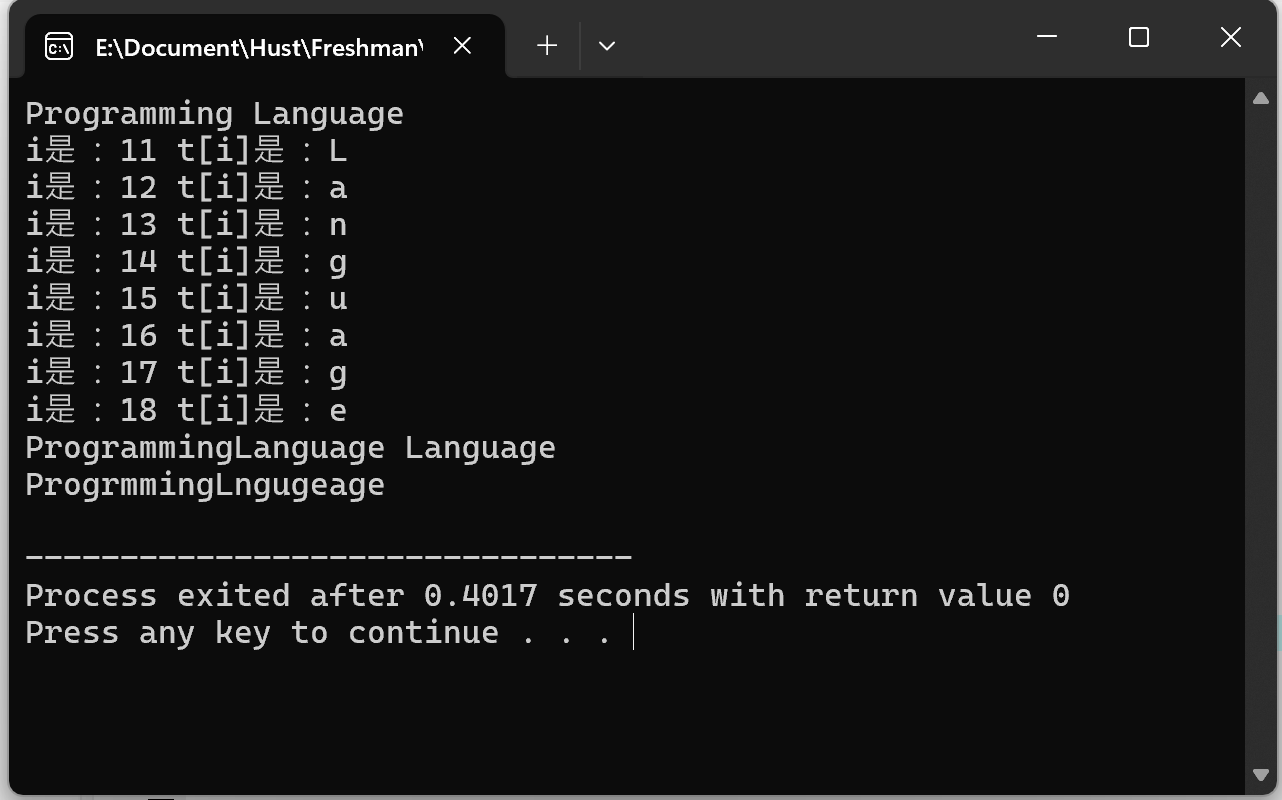
\includegraphics[scale=0.60]{images/5-1-1.png}
			\caption{執行示例}
			\label{pic5-1-1}
		\end{center}
	\end{figure}
	如结果所示，程序成功地把「Language」拼接到字符串后面，完善了strcate的功能\\
	\\
	(2)跟踪进入函数strdelc时,观察字符数组s中的内容和字符c的值,分析结果是否正确。单步执行for语句过程中,观察字符数组s、j和k值的变化,分析该结果是否存在问题。当单步执行光条落在strdele函数块结束标记所在行时，字符串s为何值?分析是否实现了所要求的删除操作。\\
	思路：\\
		我們利用迴圈把每次的狀態輸出即可(\ref{pic5-1-2})。
			\begin{figure}[H]
			\begin{center}
				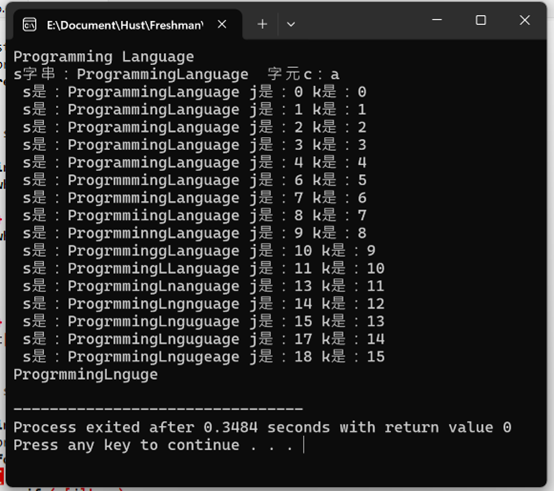
\includegraphics[scale=0.80]{images/5-1-2.png}
				\caption{執行示例}
				\label{pic5-1-2}
			\end{center}
		\end{figure}
	
	这里(\ref{pic5-1-2})虽然看上去似乎有点乱，但其实就是不断在替换字符，当遇到目标字符时就跳过字符，这时的k也不会自增，设计这两个变量J、k，j负责遍历字符串，k负责对字符串实现替换操作。
	\\
	总的来说，在对程序进行修整后，跟踪调试出来的结果亦是正常的。注意到目前处理的数据都是自定义常量，要使这个程序足以成为一个「工具」还需加入客户端输入的功能，亦即是头歌设计的要求，要满足此条件，在原有的程序上加入「scanf」输入命令即可。
	以下为头歌要求的代码(\ref{lst:5-1-10})：\\
	\begin{lstlisting}[style=commonCodeStyle, caption={示例}, label={lst:5-1-10}]
	#include <stdio.h>
	#include <stdlib.h>
	#include <string.h>
	void strcate(char t[], char s[]);
	void strdelc(char s[], char c);
	int main()
	{
		char a[100], b[100];
		char c;
		scanf("%s %s %c", b, a, &c);
		strcate(b, a);
		printf("%s\n", b);
		strdelc(b, c);
		printf("%s\n", b);
		return 0;
	}
	void strcate(char t[], char s[])
	{
		int i = 0, j = 0;
		while (t[i]!= '\0') {
			i++;
		}
		while (s[j]!= '\0') {
			t[i++] = s[j++];
		}
		t[i] = '\0';
	}
	void strdelc(char s[], char c)
	{
		int j, k;
		for (j = k = 0; s[j]!= '\0'; j++) {
			if (s[j]!= c) {
				s[k++] = s[j];
			}
		}
		s[k] = '\0';
	}
	\end{lstlisting}

\newpage

		\subsection{程序完善与修改替换}
			\subsubsection{5-2 去掉重复字符}
			\subsubsubsection{目标内容}
			(1)在一些文本数据处理中,希望去掉重复(简称去重)的字符,仅保留首次出现的字符。下面的程序能够删除字符串中的重复字符。例如源串为12eerer,去重后为12er。程序采用二重循环,大循环每次从字符串中取出一个字符,小循环遍历串中该字符后面的所有字符,若有重复的字符,则将后面的字符设置为空字符\textbackslash0。
			\\请在源程序中的下画线处填写合适的代码来完善该程序(\ref{lst:5-2-1})。
				\begin{lstlisting}[style=commonCodeStyle, caption={示例}, label={lst:5-2-1}]
				#include<stdio.h>
				#include<string.h>
				void RemoveDuplicate(char *s);
				int main()
				{
					char str[200];
					while(fgets(str, 200, stdin) != NULL)
					{
						RemoveDuplicate(str);
						printf("%s", str);
					}
					return 0;
				}
				
				void RemoveDuplicate(char *s)
				{
					int r, w, i, len;
					len = strlen(s);
					for (r = w = 0; r < len; r++)
					{
						if (s[r]!= '\0')
						{
							s[w] = s[r];
							w++;
							for (i = r + 1; i < len; i++)
							{
								if (s[i] == s[r])
								{
									s[i] = '\0';
								}
							}
						}
					}
					s[w] = '\0';
				}
			\end{lstlisting}
			執行結果(\ref{pic5-2-1})：
			\begin{figure}[H]
				\begin{center}
					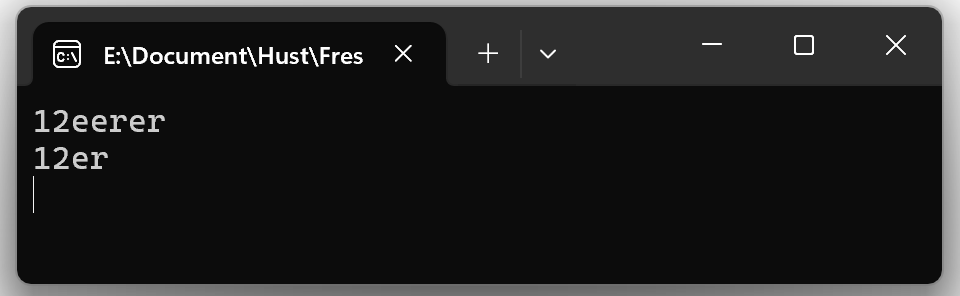
\includegraphics[scale=0.80]{images/5-2-1.png}
					\caption{執行示例}
					\label{pic5-2-1}
				\end{center}
			\end{figure}
			说明：\\
			可见这里的代码是没有问题的，能够顺利完成去重的操作。
			这里代码的设计思路和刚才那题相似，设计了二重循环，外部循环负责遍历字符串，内部循环负责判断能否去重，但同时内部循环的设计同时使用遍历去设计，使得程序的时间复杂度大大增加，面对大量数据时尤为明显。
			
			
			\subsubsection{5-3 去掉重复字符}
			\subsubsubsection{目标内容}
			(2)上面程序的时间复杂度为O(n2)。可以采用空间换时间的方法,提高处理的时间效单。具体方法为:假设待处理文本都为ASCII码字符(共256个),设置一个大小为256的标记数组，记录每个字符是否已出现过，每遇到一个字符,根据该字符的ASCII码值，将数组财应元素置为1。所以,判断一个字符是否重复,只需检查标记数组中相应位置上的值。请采用标记数组法修改RemoveDuplicate函数，使用一重循环实现字符去重，使其时间复杂度为0(n)
			\begin{lstlisting}[style=commonCodeStyle, caption={示例}, label={lst:5-2-1}]
			#include <stdio.h>
			#include <string.h>
			void RemoveDuplicate(char *s);
			int main()
			{
				char str[200];
				while (fgets(str, 200, stdin)!= NULL)
				{
					RemoveDuplicate(str);
					printf("%s", str);
				}
				return 0;
			}
			void RemoveDuplicate(char *s)
			{
				int i, len;
				len = strlen(s);
				int mark[256] = {0};
				int w = 0;
				for (i = 0; i < len; i++)
				{
					int ascii_index = (int)s[i];
					if (mark[ascii_index] == 0)
					{
						mark[ascii_index] = 1;
						s[w++] = s[i];
					}
				}
				s[w] = '\0';
			}
			\end{lstlisting}
		執行結果(\ref{pic5-3-1})：
		\begin{figure}[H]
			\begin{center}
				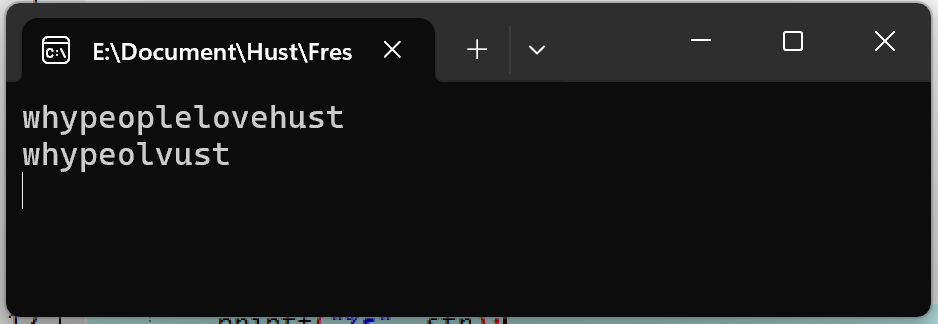
\includegraphics[scale=0.80]{images/5-3-1.png}
				\caption{執行示例}
				\label{pic5-3-1}
			\end{center}
		\end{figure}
	这个设计同样是能够顺利去重的。\\
	这里按照替代方案的思路设计了一个判断被存入字符是否己被输入过的数组，这个数组主要以放入0/1布尔值去作为条件句执行。同样能够实现去重的操作，但相比起原来的内部循环更简化了时间复杂度。
	
			\subsubsection{5-4 约瑟夫问题(一)}
			\subsubsubsection{目标内容}
			(1)下面的源程序用于求解约瑟夫问题:M个人围成一圈,从第一个人开始依次从1至N循环报数，每当报数为N时报数人出圈,直到圈中只剩下一个人为止。\\
			相关代码(\ref{lst:5-4-1})：
			\begin{lstlisting}[style=commonCodeStyle, caption={示例}, label={lst:5-4-1}]
			#include <stdio.h>
			#define M 10
			#define N 3
			int main(void)
			{
				int a[M], b[M];
				int i, j, k;
				for (i = 0; i < M; i++)
				{
					a[i] = i + 1;
				}
				for (i = M, j = 0; i > 1; i--)
				{
					for (k = 1; k <= N; k++)
					{
						if (++j > i - 1)
						j = 0;
					}
					b[M - i] = j? a[j - 1] : a[i - 1];  
					if (j)
					{
						for (k = --j; k < i - 1; k++)  
						{
							a[k] = a[k + 1];  
						}
					}
					else
					{
						for (k = i - 1; k > 0; k--)
						{
							a[k] = a[k - 1];
						}
					}
				}
				for (i = 0; i < M - 1; i++)
				{
					printf("%6d", b[i]);
				}
				printf("%6d\n", a[0]);
				return 0;
			}
			\end{lstlisting}
			输出结果：\\
			\begin{figure}[H]
				\begin{center}
					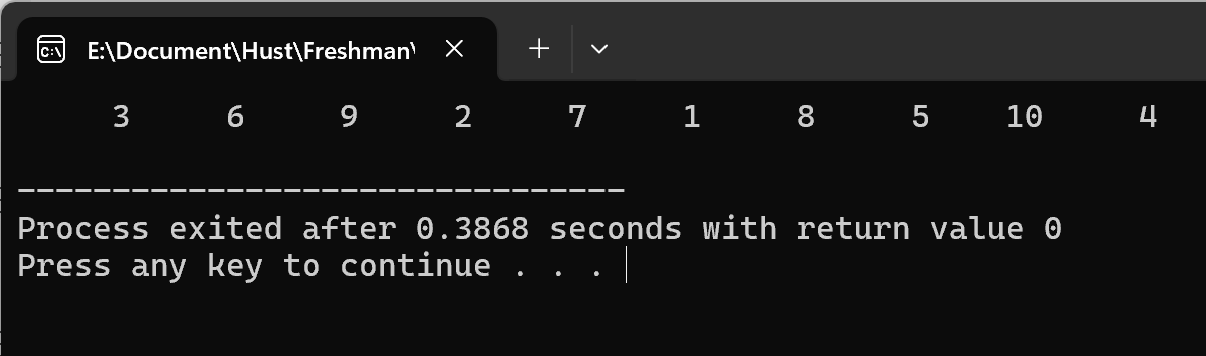
\includegraphics[scale=0.80]{images/5-4-1.png}
					\caption{執行示例}
					\label{pic5-4-1}
				\end{center}
			\end{figure}
			这里(\ref{pic5-4-1})定义了「M=10」、「N=3」去进行约瑟夫问题，从输出结果来看这段代码是正确的，能够顺利执行。
			\\这段代码中，外层的 for 循环 for (i = M, j = 0; i > 1; i--) 控制整个出圈的过程，i 初始化为 M 表示初始圈里有 M 个人，随着每次有人出圈，i 的值会减 1，直到圈里只剩下 1 个人（即 i > 1 这个条件不满足时循环结束），j 用于记录当前报数的人的位置（下标），初始化为 0。
			\\中层的 for 循环 for (k = 1; k <= N; k++) 用于模拟每次从 1 到 N 的报数过程。在这个循环里，if (++j > i - 1) 这个条件判断实现了循环报数的逻辑，当 j 的值（经过自增后）超过了当前圈里剩下的人数减 1（因为数组下标从 0 开始）时，就把 j 重置为 0，相当于报数到一圈的末尾后又回到开头继续报数。
			
			
			\subsubsection{5-5 约瑟夫问题(二)}
			\subsubsubsection{目标内容}
			(2)上面的程序使用数组元素的值表示圈中人的编号,故每当有人出圈时都要压缩数组，这种算法不够精练。如果采用做标记的办法,即每当有人出圈时对相应数组元素做标,从而可省掉压缩数组的时间,这样处理效率会更高，请采用做标记的办法修改程序、使修改后的程序与原程序具有相同的功能。\\
			相关代码(\ref{lst:5-5-1})：
			\begin{lstlisting}[style=commonCodeStyle, caption={示例}, label={lst:5-5-1}]
			#include <stdio.h>
			#define M 10
			#define N 3
			int main(void)
			{
				int a[M];
				int flag[M]; 
				int i, j, k;
				for (i = 0; i < M; i++)
				{
					a[i] = i + 1;
					flag[i] = 0;
				}
				j = -1; 
				for (i = M; i > 1; i--)
				{
					for (k = 1; k <= N; k++)
					{
						do
						{
							j = (j + 1) % M;
						} while (flag[j]);
					}
					flag[j] = 1;
					printf("%6d", a[j]);
				}
				for (i = 0; i < M; i++)
				{
					if (flag[i] == 0)
					{
						printf("%6d\n", a[i]);
						break;
					}
				}
				return 0;
			}
			\end{lstlisting}
			输出结果：\\
			\begin{figure}[H]
				\begin{center}
					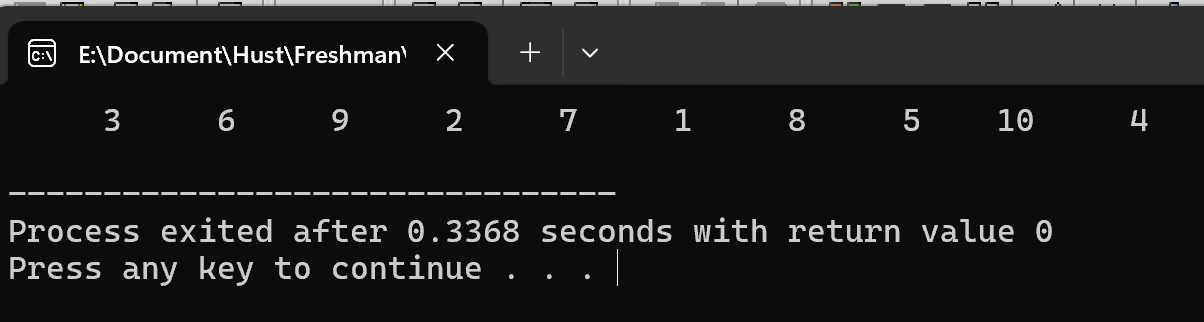
\includegraphics[scale=0.80]{images/5-5-1.png}
					\caption{執行示例}
					\label{pic5-5-1}
				\end{center}
			\end{figure}
			分析：\\
			在这段代码(\ref{pic5-5-1})中，通过定义两个数组 a 和 flag 以及相应的循环逻辑来实现这个过程。和上一题不同的是，数组 flag 用于标记每个人是否出圈，初始时通过循环将 flag 数组的所有元素都赋值为 0，表示所有人都还未出圈。
			\\而 while (flag[j]) 这个条件是为了跳过那些已经被标记出圈（对应 flag 数组中元素值为 1）的位置，保证报数是针对未出圈的人进行的。而这里把「j=0」改成「j = (j + 1) % M;」能够避免数越界的问题。下面再把程序改成能够通过用户自定义M、N变量的形式。
			
			\\
			相关代码(\ref{lst:5-5-2})：
			\begin{lstlisting}[style=commonCodeStyle, caption={示例}, label={lst:5-5-2}]
				#include <stdio.h>
				int main(void)
				{
					int M,N;
					scanf("%d %d",&M,&N);
					int a[M];
					int flag[M]; 
					int i, j, k;
					for (i = 0; i < M; i++)
					{
						a[i] = i + 1;
						flag[i] = 0;
					}
					
					j = -1;
					for (i = M; i > 1; i--)
					{
						for (k = 1; k <= N; k++)
						{
							do
							{
								j = (j + 1) % M;
							} while (flag[j]);
						}
						flag[j] = 1;
						printf("%6d", a[j]);
					}
					for (i = 0; i < M; i++)
					{
						if (flag[i] == 0)
						{
							printf("%d\n", a[i]);
							break;
						}
					}
					return 0;
				}
				
			\end{lstlisting}
		\newpage
			
		\subsection{程序设计}
			\subsubsection{5-6 整数的二进制表示}
			\subsubsubsection{目标内容}
			输入一个整数，将它在内存中的二进制表示的每一位转换成对应的数字字符并且存放到一个字符数组中，然后输出该整数的二进制表示（32位有符号整数，输出每4位用空格分隔）。
			\subsubsubsection{分析}
			要实现输入一个整数，将其转换为 32 位有符号整数的二进制表示（每 4 位用空格分隔）并输出的功能，整体思路是利用位运算按位提取该整数的二进制位信息，转换为字符后存入数组，再按格式要求输出数组内容。\\
			思路：\\
			1. 获取一个用户端的整数型数据。\\
			2.转换过程\\
			使用按位操作逐位检查整数的每一位。将每一位的结果存储在一个字符数组单元中。
			\\可用三目运算符快速判断和赋值\\
			3.格式化输出\\
			在每4位之间添加一个空格。\\
			    用取模即可；如「i%4==0」\\
			printf打印最终的二进制字符串\\
			
			流程图：\\
			这里主要设计一个总流程图(\ref{pic5-6-1})和按位操作及存取时的流程图(\ref{pic5-6-2})以演示程序的运行。\\
			首先是总流程，本题的总流程图较为单一，为一个单向无分支的操作。固能够简单容易地理解，大致上和上面思路的形容差不多，先获取数据，然后按位操作判断，最后作输出
			\begin{figure}[H]
				\begin{center}
					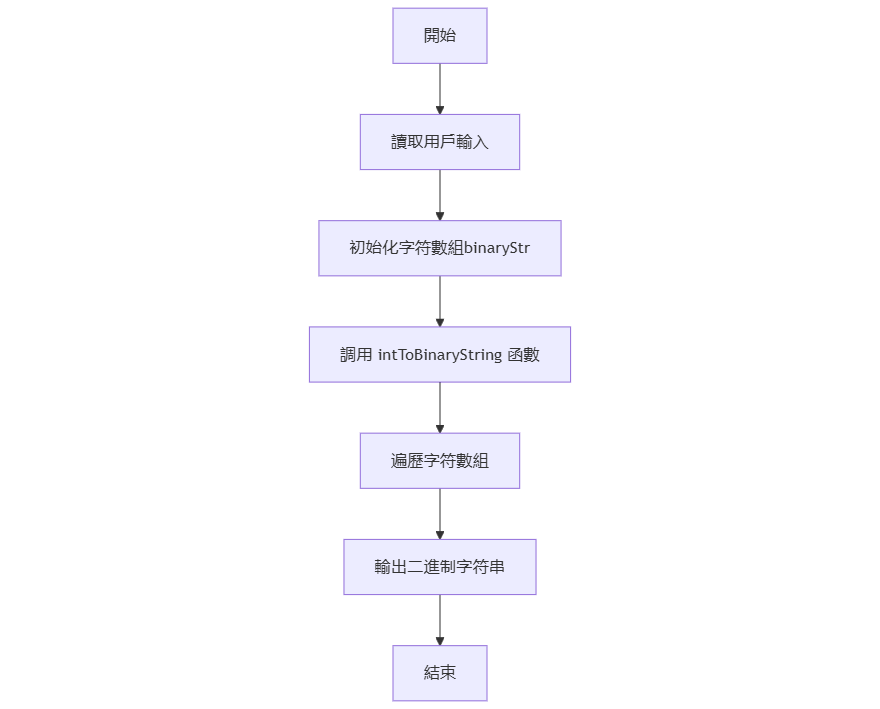
\includegraphics[scale=0.50]{images/5-6-1.png}
					\caption{流程图}
					\label{pic5-6-1}
				\end{center}
			\end{figure}
			\begin{figure}[H]
			\begin{center}
				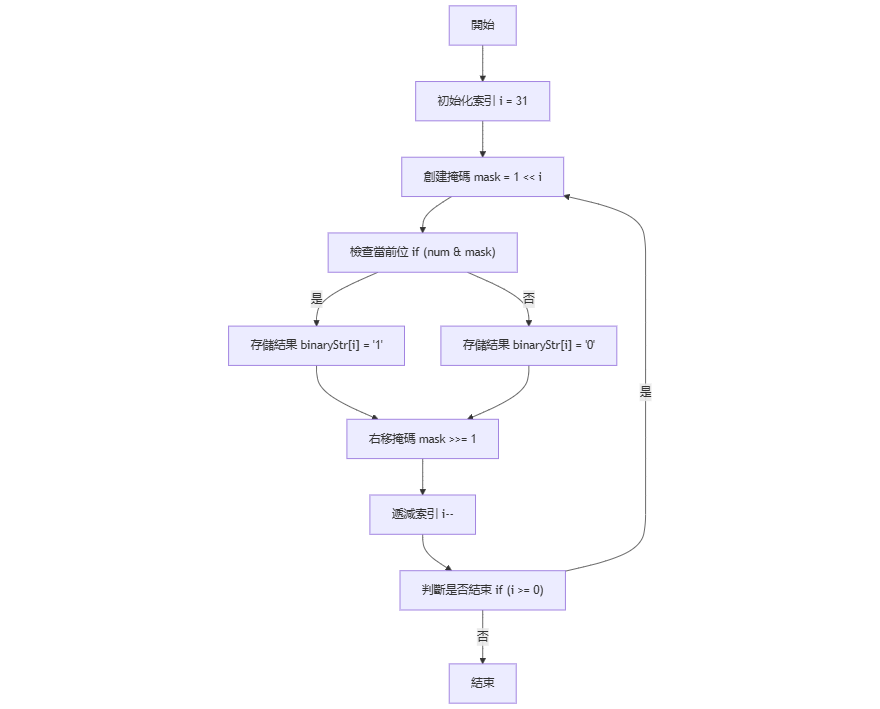
\includegraphics[scale=0.50]{images/5-6-2.png}
				\caption{流程图}
				\label{pic5-6-2}
			\end{center}
		\end{figure}
			
			
			\subsubsubsection{相关代码(\ref{lst:5-6-1})}

			\begin{lstlisting}[style=commonCodeStyle, caption={示例}, label={lst:5-6-1}]
			#include <stdio.h>
			#include <stdlib.h>
			#define BITS 32
			void intToBinaryString(int num, char binaryStr[]) {
				int i;
				for (i = BITS - 1; i >= 0; i--) {
					binaryStr[i] = (num & (1 << (BITS - 1 - i)))? '1' : '0';
				}
				binaryStr[BITS] = '\0';
			}
			int main() {
				int num;
				char binaryStr[BITS + 1];
				scanf("%d", &num);
				intToBinaryString(num, binaryStr);
				for (int i = 0; i < BITS; i++) {
					printf("%c", binaryStr[i]);
					if ((i + 1) % 4 == 0 && i!= BITS - 1) {
					printf(" ");
				}
			}
			printf("\n");
			return 0;
		}
			\end{lstlisting}
			
			\subsubsubsection{执行结果}
			执行结果(\ref{pic5-6-3}\ref{pic5-6-4})
			\begin{figure}[H]
				\begin{center}
					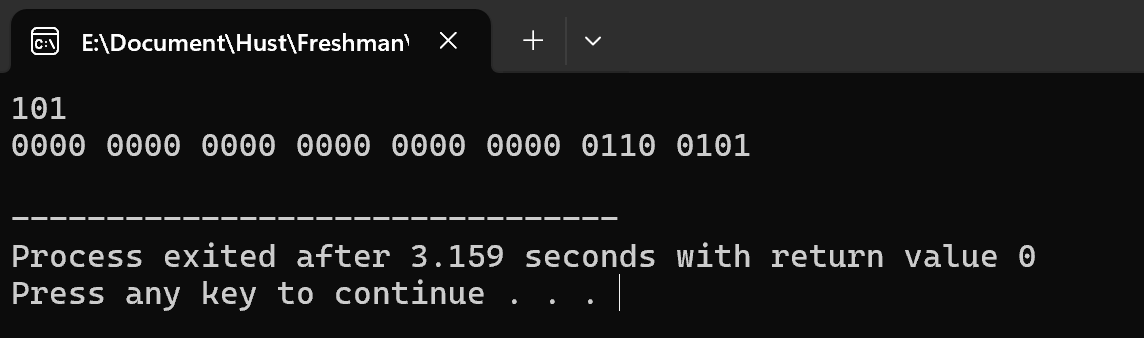
\includegraphics[scale=0.70]{images/5-6-3.png}
					\caption{执行示例}
					\label{pic5-6-3}
				\end{center}
			\end{figure}
		\begin{figure}[H]
			\begin{center}
				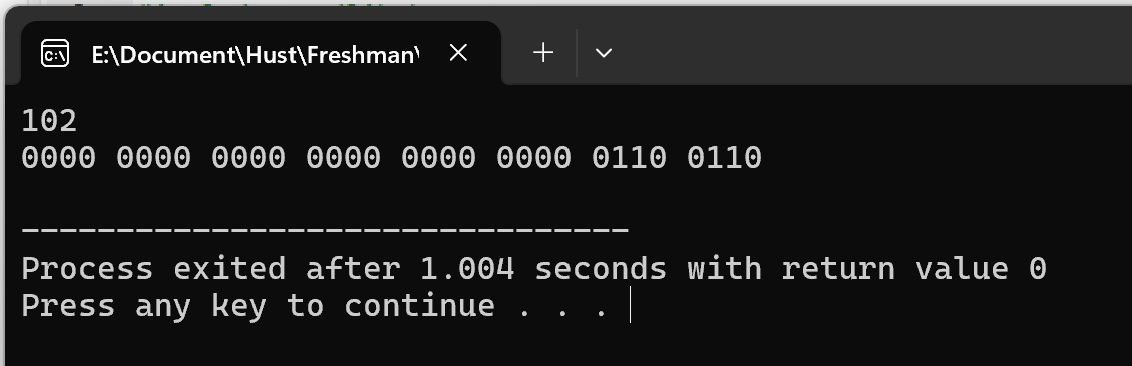
\includegraphics[scale=0.70]{images/5-6-4.png}
				\caption{执行示例}
				\label{pic5-6-4}
			\end{center}
		\end{figure}

\newpage
			
			\subsubsection{5-7 成绩排序}
			\subsubsubsection{目标内容}
			(1)	输入一个整数,将它在内存中二进制表示的每一位转换成对应的数字字符并且存放到一个字符数组中,然后输出该整数的二进制表示。	\\
			(2)编写一个C程序，要求采用模块化程序设计思想,将相关功能用函数实现,并提供菜单选项。该程序具有以下功能:\\
		    	1.输人n个学生的姓名和C语言课程的成绩。\\
		    	2.将成绩按从高到低的次序排序,姓名同时进行相应调整。\\
		    	3.输出所有学生的姓名和C语言课程的成绩。\\
			
			
			\subsubsubsection{分析}
			整个程序可以用模块化设计思想，将不同的功能封装到不同的函数中，通过一个菜单来让用户选择具体要执行的功能，这样使得程序结构清晰、易于维护和扩展。主函数主要负责展示菜单以及根据用户选择调用相应的功能函数来完成操作。\\
			总流程图(\ref{pic5-7-1})：
			\begin{figure}[H]
				\begin{center}
					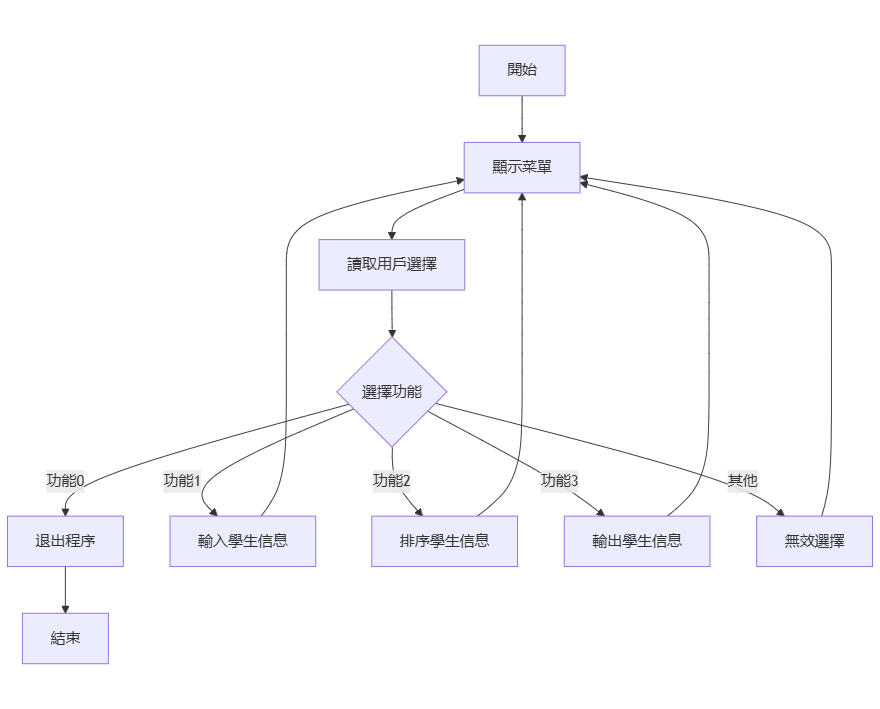
\includegraphics[scale=0.40]{images/5-7-1.png}
					\caption{流程图}
					\label{pic5-7-1}
				\end{center}
			\end{figure}
			設計思路：\\
			1.输入学生信息功能实现思路：\\
			函数设计：创建 void 函数，用于输入 n 个学生的姓名和 C 语言课程成绩。函数可以接收学生数量 n 作为参数，在函数内部定义合适的数组（比如字符数组存储姓名，整型数组存储成绩）来存放数据，通过循环让用户依次输入每个学生的姓名和成绩，完成信息的收集工作。\\
			相关流程图(\ref{pic5-7-2})：
			\begin{figure}[H]
				\begin{center}
					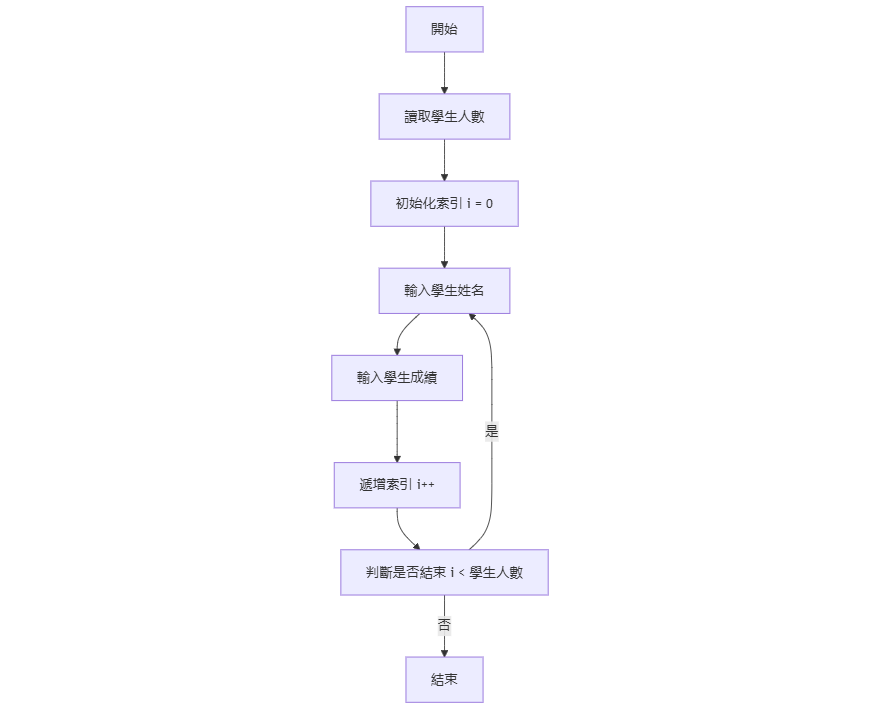
\includegraphics[scale=0.60]{images/5-7-2.png}
					\caption{流程图}
					\label{pic5-7-2}
				\end{center}
			\end{figure}
			
			2.成绩排序及姓名相应调整功能实现思路：\\
			函数设计：设计 void 函数，该函数接收存储成绩和姓名的数组以及学生数量 n 作为参数，其目的是根据成绩对学生信息进行排序。可以采用常见的排序算法，比如冒泡排序、快速排序等，在比较成绩的同时，当交换成绩的顺序时，对应的学生姓名也要进行交换，以保证成绩和姓名始终是对应的，最终实现成绩从高到低排序且姓名同步调整的效果。\\
			相关流程图(\ref{pic5-7-3})：
			\begin{figure}[H]
				\begin{center}
					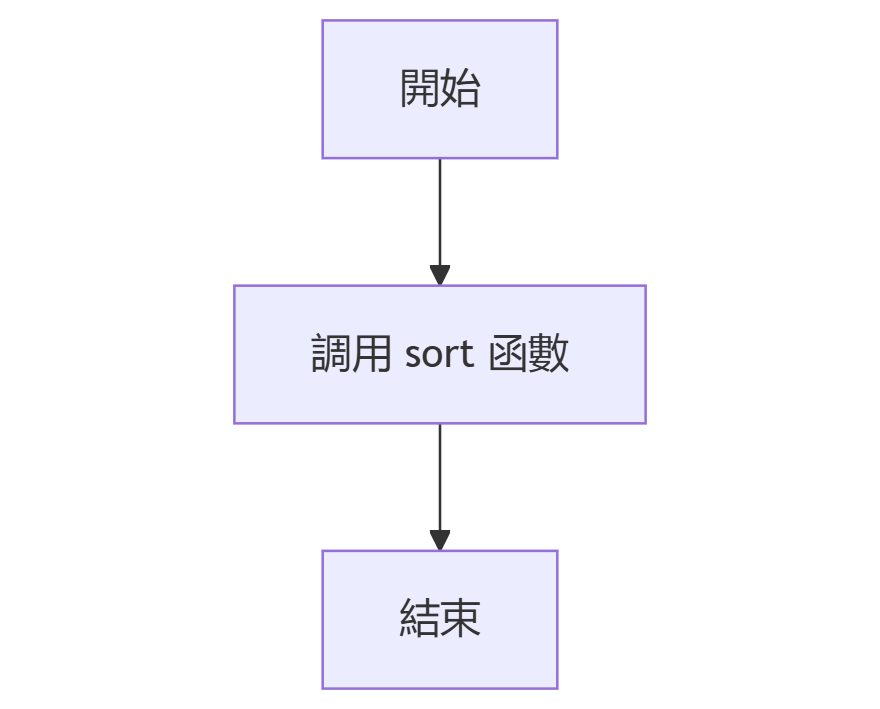
\includegraphics[scale=0.30]{images/5-7-3.png}
					\caption{流程图}
					\label{pic5-7-3}
				\end{center}
			\end{figure}
			
			3.输出学生信息功能实现思路：\\
			函数设计：构建 void函数，它接收存储学生信息的数组以及学生数量 n 作为参数，通过循环遍历数组，将每个学生的姓名和成绩按照一定格式输出，方便查看所有学生的相关信息。\\
			相关流程图(\ref{pic5-7-4}):
			\begin{figure}[H]
				\begin{center}
					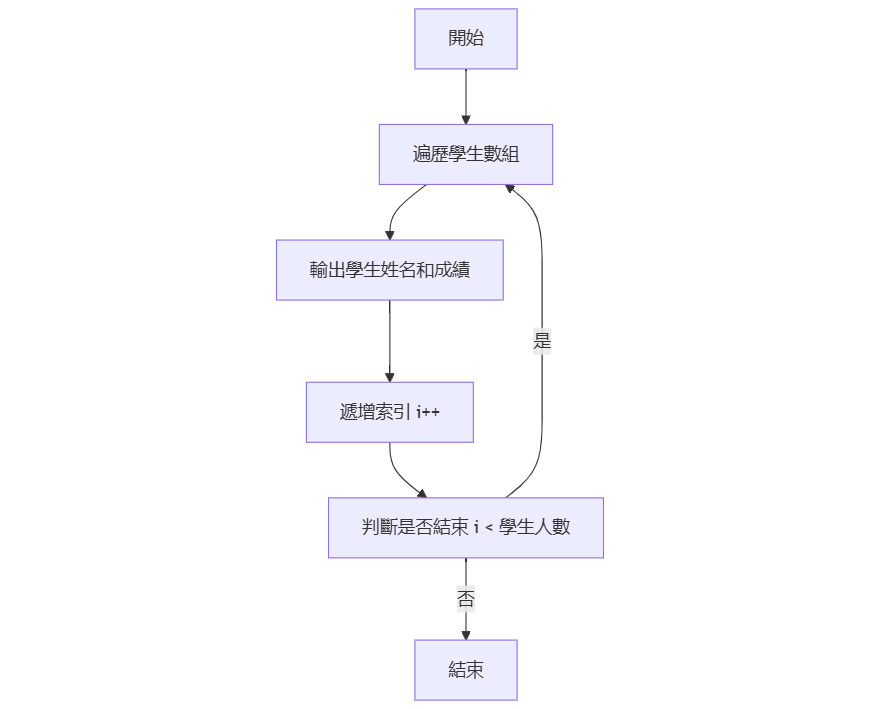
\includegraphics[scale=0.40]{images/5-7-4.png}
					\caption{流程图}
					\label{pic5-7-4}
				\end{center}
			\end{figure}
			
			\subsubsubsection{相关代码}
			相关代码(\ref{lst:5-7-1})：
		\begin{lstlisting}[style=commonCodeStyle, caption={示例}, label={lst:5-7-1}]
		#include <stdio.h>
		#include <stdlib.h>
		#include <string.h>
		#define MAX_STUDENTS 100
		#define MAX_NAME_LENGTH 50
		typedef struct {
			char name[MAX_NAME_LENGTH];
			int score;
		} Student;
		void inputStudents(Student students[], int n);
		void sortStudents(Student students[], int n);
		void outputStudents(Student students[], int n);
		int main() {
			Student students[MAX_STUDENTS];
			int choice, n;
			do {
				scanf("%d", &choice);
				
				switch (choice) {
					case 1:
					scanf("%d", &n);
					inputStudents(students, n);
					break;
					case 2:
					sortStudents(students, n);
					break;
					case 3:
					outputStudents(students, n);
					break;
					case 0:
					break;
				}
			} while (choice!= 0);
			return 0;
		}
		void inputStudents(Student students[], int n) {
			for (int i = 0; i < n; i++) {
				
				scanf("%s %d", students[i].name, &students[i].score);
			}
		}
		void sortStudents(Student students[], int n) {
			for (int i = 0; i < n - 1; i++) {
				for (int j = i + 1; j < n; j++) {
					if (students[i].score < students[j].score) {
						int tempScore = students[i].score;
						students[i].score = students[j].score;
						students[j].score = tempScore;
						char tempName[MAX_NAME_LENGTH];
						strcpy(tempName, students[i].name);
						strcpy(students[i].name, students[j].name);
						strcpy(students[j].name, tempName);
					} else if (students[i].score == students[j].score) {
						if (strcmp(students[i].name, students[j].name) > 0) {
							
							char tempName[MAX_NAME_LENGTH];
							strcpy(tempName, students[i].name);
							strcpy(students[i].name, students[j].name);
							strcpy(students[j].name, tempName);
							int tempScore = students[i].score;
							students[i].score = students[j].score;
							students[j].score = tempScore;
						}
					}
				}
			}
		}
		void outputStudents(Student students[], int n) {
			for (int i = 0; i < n; i++) {
				printf("%s %d\n", students[i].name, students[i].score);
			}
		}
		\end{lstlisting}
			
			
			\subsubsubsection{执行结果}
			\begin{figure}[H]
				\begin{center}
					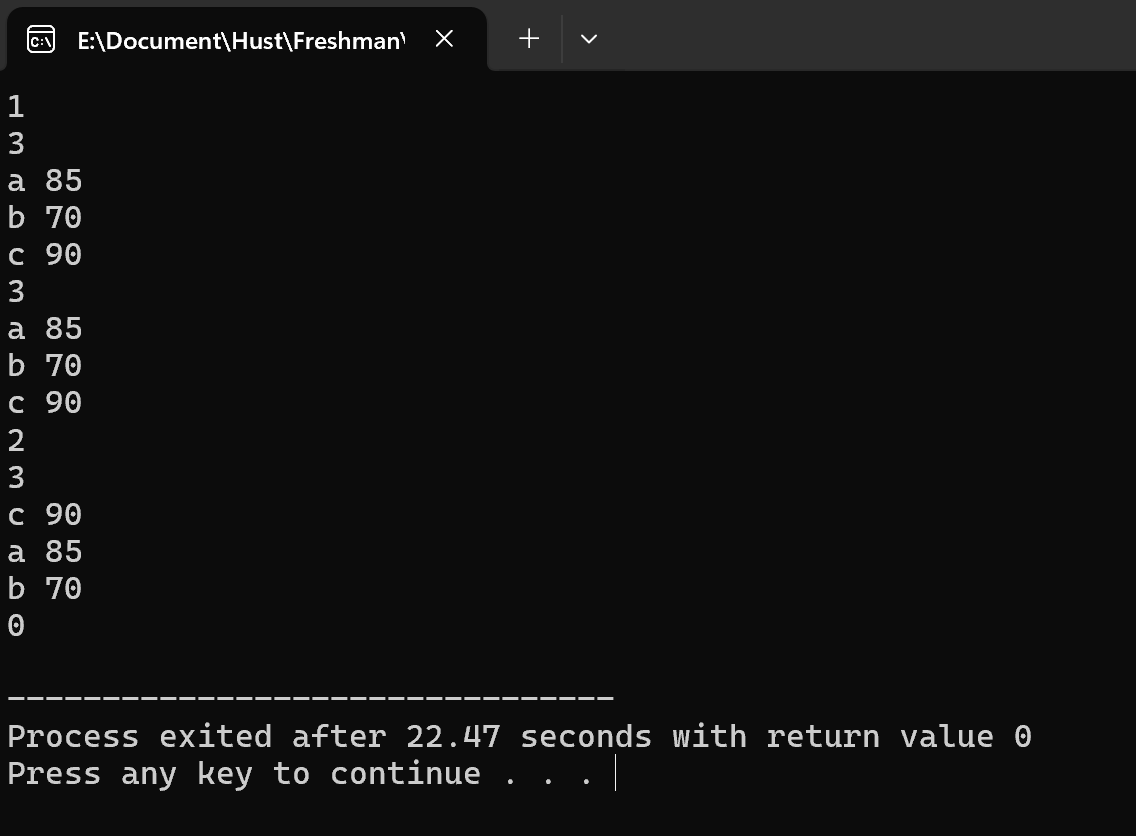
\includegraphics[scale=0.70]{images/5-7-5.png}
					\caption{执行示例}
					\label{pic5-7-5}
				\end{center}
			\end{figure}
		分析：\\
		    可以见到先是进行了功能1，输入了3名学生的姓名和成绩，然后通过3直接输出，再测试排序的功后输入了2之后再进行输出，可见是成功排序的。
		    \\这里的代码大致可分为四个模块去观察，主函数及三功能函数部分，首先是利用switch语句去实现分块处理，定义了一个structure结构去存放学生姓名和成绩。通过for循环依次存入。然后在排序模块中通过创建temp变量和if条件句去进行交换内容和排序，最后输出部分则是简单的回环输出。
		    \\由此可见，把复杂的程序要求对其分块处理可以使得程序思路变得清晰，亦能更于理解读写，在除错了亦能更快定位到错处，因此养成一个模块化的思想方向可以有助于我们编程的思路。
		
			
			
			\subsubsection{5-8 二分查找}
			\subsubsubsection{目标内容}
			在5-7的基础上增加查找功能（功能编号4）：输入一个C语言课程成绩值，用二分查找进行搜索。如果查找到有该成绩，则输出该成绩所有学生的姓名和C语言课程的成绩；否则，输出提示"not found"。
			\subsubsubsection{分析}
			在原有主程序switch部分加入一个case 4，然后构建二分查找法相关的函数。在使用二分法查找时要先对成绩进行排序，排序后再查找。
			总流程图(\ref{pic5-8-1})：
			\begin{figure}[H]
				\begin{center}
					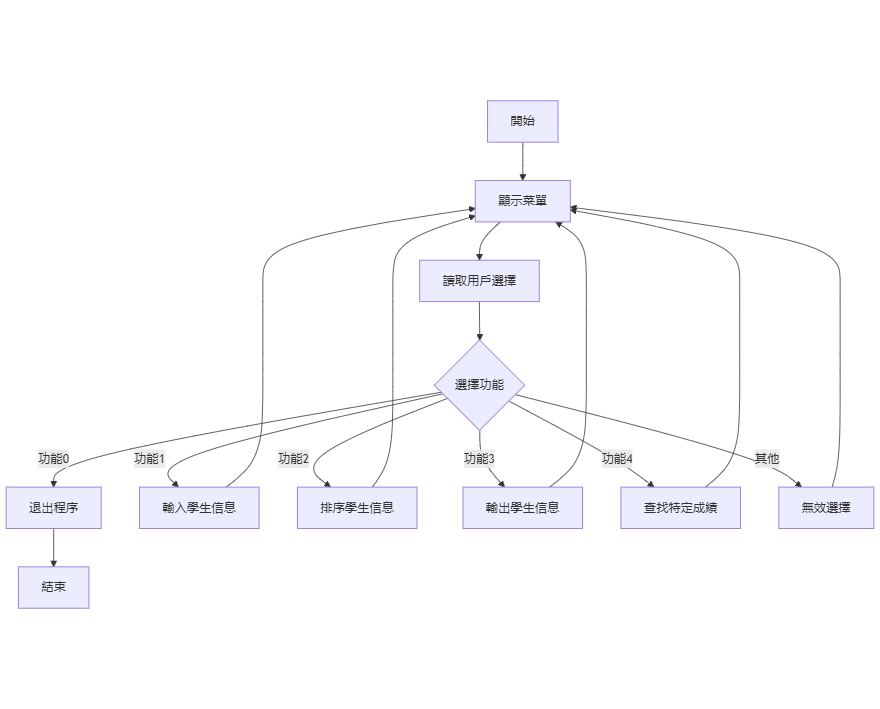
\includegraphics[scale=0.50]{images/5-8-1.png}
					\caption{流程圖}
					\label{pic5-8-1}
				\end{center}
			\end{figure}
			这里使用 while 循环来实现二分查找的核心逻辑，只要 left 小于等于 right，就意味着还有可能在当前界定的范围内找到目标成绩，循环会持续进行\\。
			在每次循环中，首先通过 int mid = left + (right - left) / 2; 计算中间位置 mid。这种计算方式可以避免直接使用 (left + right) / 2 时可能出现的整数溢出问题（当 left 和 right 的数值较大时），确保能正确获取中间索引。\\
			然后通过 if-else if 条件语句来根据中间位置元素（students[mid].score）与目标成绩 target 的比较结果决定下一步操作：\\
			相关流程图(\ref{pic5-8-2})：	
			\begin{figure}[H]
				\begin{center}
					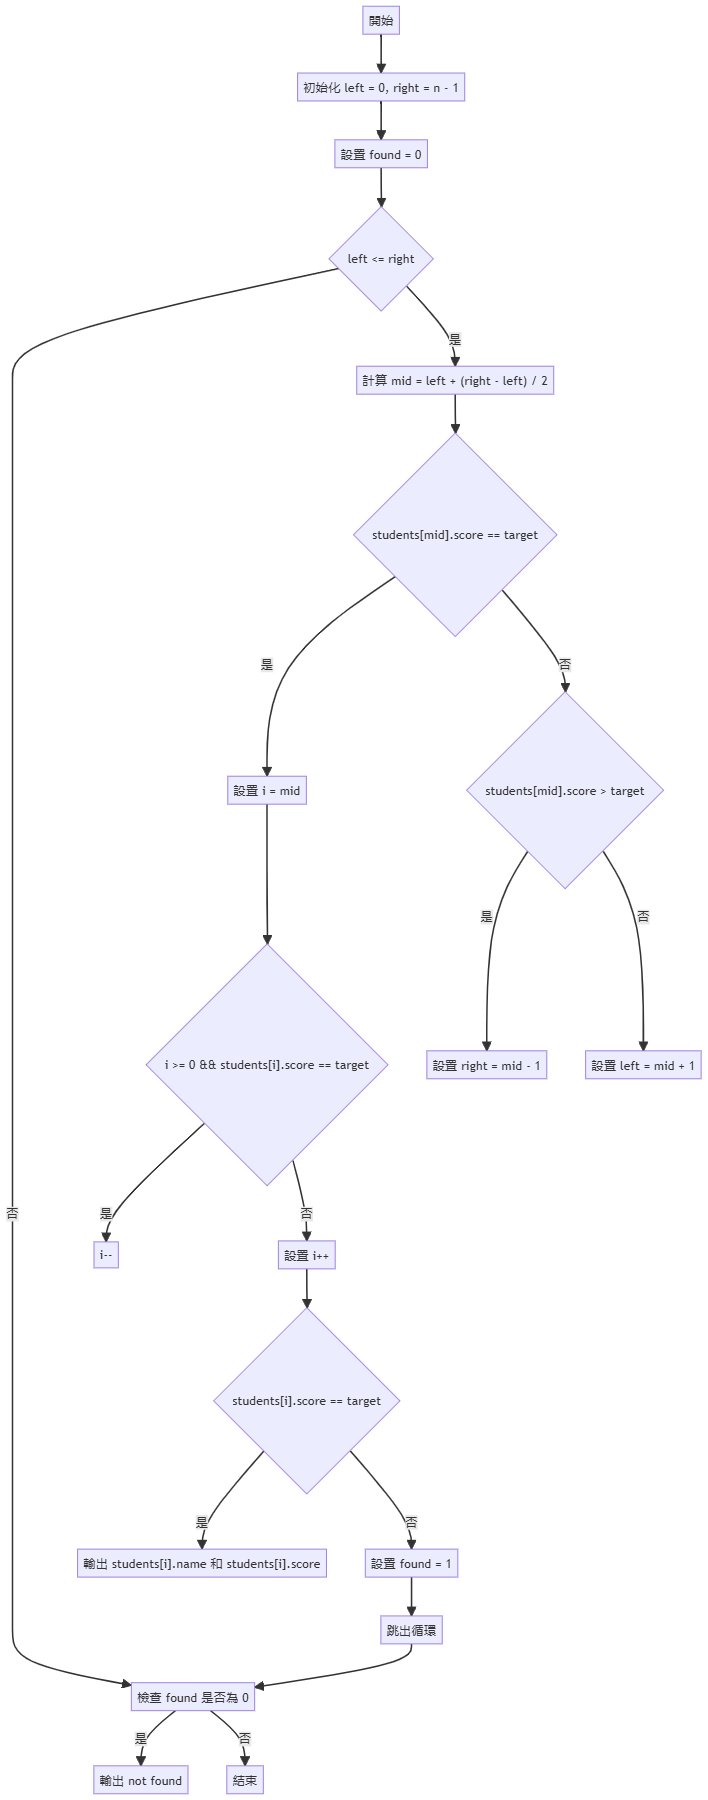
\includegraphics[scale=0.35]{images/5-8-2.png}
					\caption{流程圖}
					\label{pic5-8-2}
				\end{center}
			\end{figure}
			
			\subsubsubsection{相关代码}
			相关代码(\ref{lst:5-8-1})：
			\begin{lstlisting}[style=commonCodeStyle, caption={示例}, label={lst:5-8-1}]
			#include <stdio.h>
			#include <stdlib.h>
			#include <string.h>
			#define MAX_STUDENTS 100
			#define MAX_NAME_LENGTH 50
			typedef struct {
				char name[MAX_NAME_LENGTH];
				int score;
			} Student;
			void inputStudents(Student students[], int n);
			void sortStudents(Student students[], int n);
			void outputStudents(Student students[], int n);
			void binarySearch(Student students[], int n, int target);
			int main() {
				Student students[MAX_STUDENTS];
				int choice, n;
				do {
					scanf("%d", &choice);
					;
					switch (choice) {
						case 1:
						scanf("%d", &n);
						inputStudents(students, n);
						break;
						case 2:
						sortStudents(students, n);
						break;
						case 3:
						outputStudents(students, n);
						break;
						case 4:
						{
							int target;
							scanf("%d", &target);
							binarySearch(students, n, target);
							break;
						}
						case 0:
						break;
					}
				} while (choice!= 0);
				return 0;
			}
			void inputStudents(Student students[], int n) {
				for (int i = 0; i < n; i++) {
					
					scanf("%s %d", students[i].name, &students[i].score);
				}
			}
			void sortStudents(Student students[], int n) {
				for (int i = 0; i < n - 1; i++) {
					for (int j = i + 1; j < n; j++) {
						if (students[i].score < students[j].score) {
							int tempScore = students[i].score;
							students[i].score = students[j].score;
							students[j].score = tempScore;
							char tempName[MAX_NAME_LENGTH];
							strcpy(tempName, students[i].name);
							strcpy(students[i].name, students[j].name);
							strcpy(students[j].name, tempName);
						} else if (students[i].score == students[j].score) {
							if (strcmp(students[i].name, students[j].name) > 0) {
								char tempName[MAX_NAME_LENGTH];
								strcpy(tempName, students[i].name);
								strcpy(students[i].name, students[j].name);
								strcpy(students[j].name, tempName);
								int tempScore = students[i].score;
								students[i].score = students[j].score;
								students[j].score = tempScore;
							}
						}
					}
				}
			}
			void outputStudents(Student students[], int n) {
				for (int i = 0; i < n; i++) {
					printf("%s %d\n", students[i].name, &students[i].score);
				}
			}
			void binarySearch(Student students[], int n, int target) {
				int left = 0;
				int right = n - 1;
				int found = 0;
				while (left <= right) {
					int mid = left + (right - left) / 2;
					if (students[mid].score == target) {
						int i = mid;
						while (i >= 0 && students[i].score == target) {
							i--;
						}
						i++;
						for (; i < n && students[i].score == target; i++) {
							printf("%s %d\n", students[i].name, students[i].score);
						}
						found = 1;
						break;
					} else if (students[mid].score > target) {
						right = mid - 1;
					} else {
						left = mid + 1;
					}
				}
				if (!found) {
					printf("not found\n");
				}
			}
			\end{lstlisting}
			
			\subsubsubsection{执行结果}
			执行结果(\ref{pic5-8-3}\ref{pic5-8-4})：
			\begin{figure}[H]
				\begin{center}
					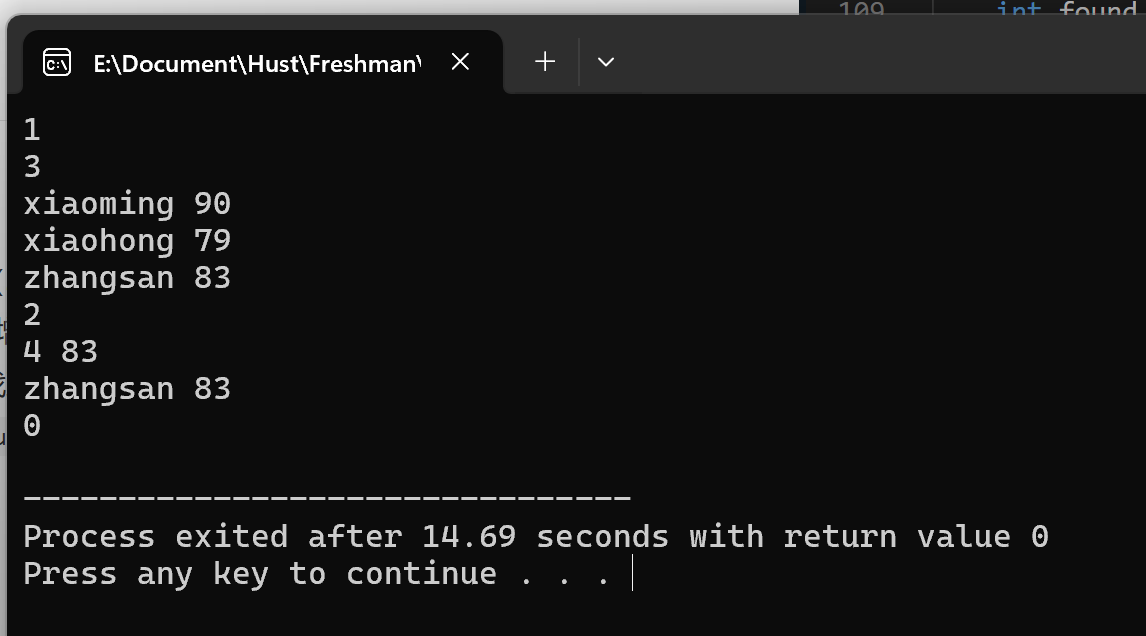
\includegraphics[scale=0.70]{images/5-8-3.png}
					\caption{执行示例}
					\label{pic5-8-3}
				\end{center}
			\end{figure}
		\begin{figure}[H]
			\begin{center}
				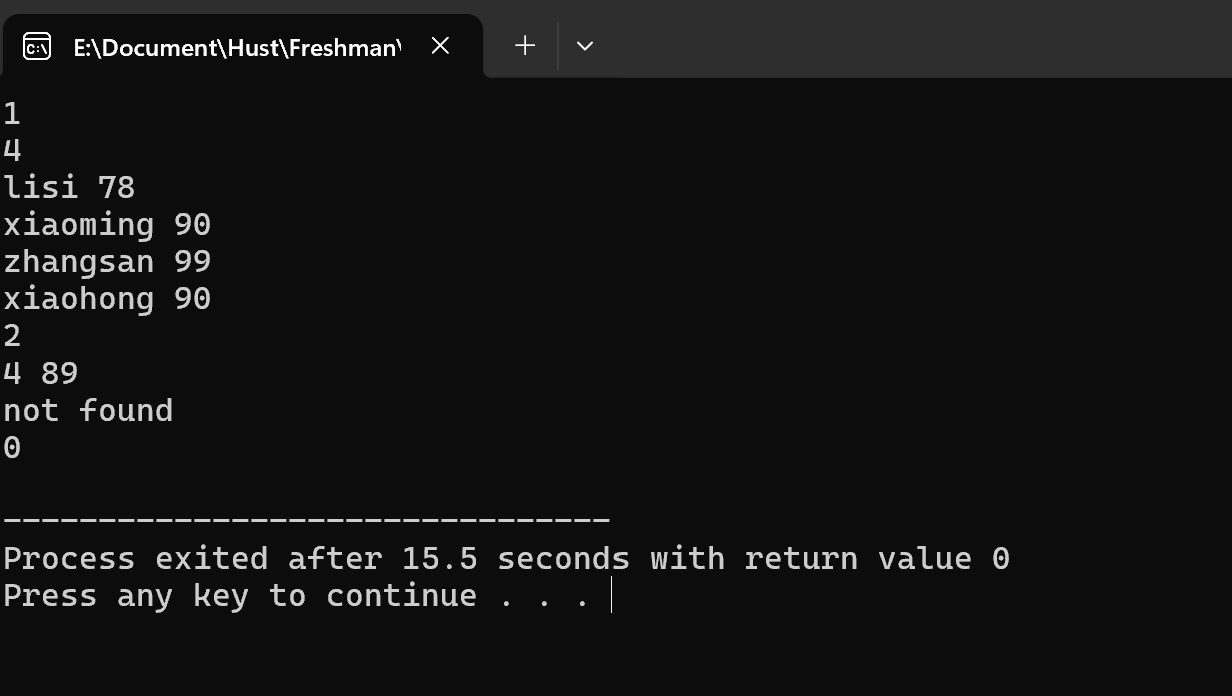
\includegraphics[scale=0.70]{images/5-8-4.png}
				\caption{执行示例}
				\label{pic5-8-4}
			\end{center}
		\end{figure}
			这里可见是先操作了排序再查找，不然的话直接使用二分查找是不一定能找到结果的，这两幅图分别显示了查找成功和查找失则的输出结果，可见该程序是满足题目的要求的。
			
			\subsubsection{5-9 插入字符串}
			
			\subsubsubsection{目标内容}
			编写函数strnins(t,s,n),其功能是：将串s插入串t串的第n个字符的后面，编写main函数测试strnins函数的正确性。
			\subsubsubsection{分析}
			题目要求实现一个名为 strnins 的函数，它需要接收三个参数，分别是两个字符串 t 和 s，以及一个表示位置的整数 n。该函数的主要功能是把字符串 s 插入到字符串 t 中第 n 个字符的后面，最终改变字符串 t 的内容以体现插入操作后的结果。\\
			总流程图(\ref{pic5-9-1})：
			\begin{figure}[H]
				\begin{center}
					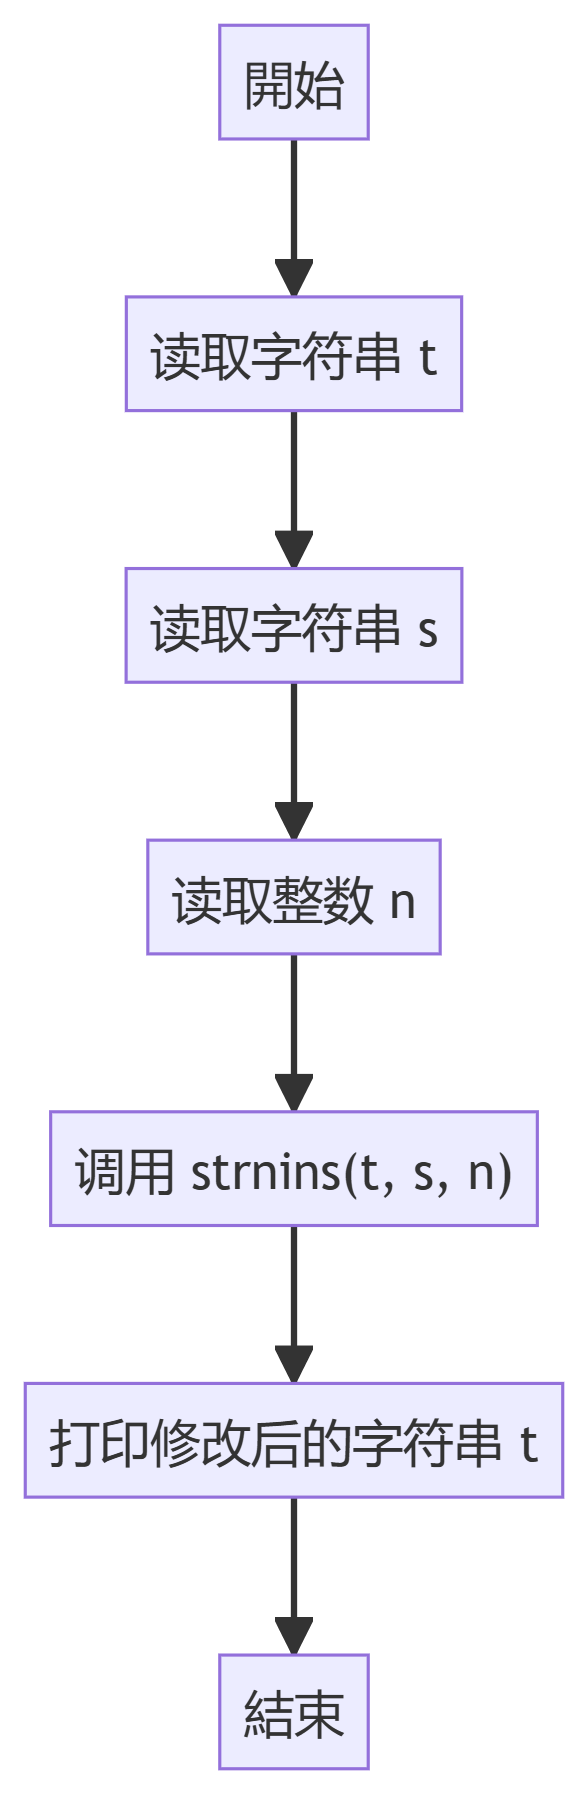
\includegraphics[scale=0.20]{images/5-9-1.png}
					\caption{流程图}
					\label{pic5-9-1}
				\end{center}
			\end{figure}
			
			設計思路：\\
			输入读取:\\
			    1.从标准输入读取两个字符串 t 和 s。\\
		   	    2.字符串插入逻辑:\\
			计算字符串 t 和 s 的长度。\\
			创建一个临时字符串 temp，其长度为 len\_t + len\_s + 1，以容纳合并后的字符串和终止符 \textbackslash0。\\
			在 temp 的末尾添加终止符 \textbackslash0。\\
			将 temp 复制回 t。
			3.输出结果\\
			
			相关流程图(\ref{pic5-9-2})：
			\begin{figure}[H]
				\begin{center}
					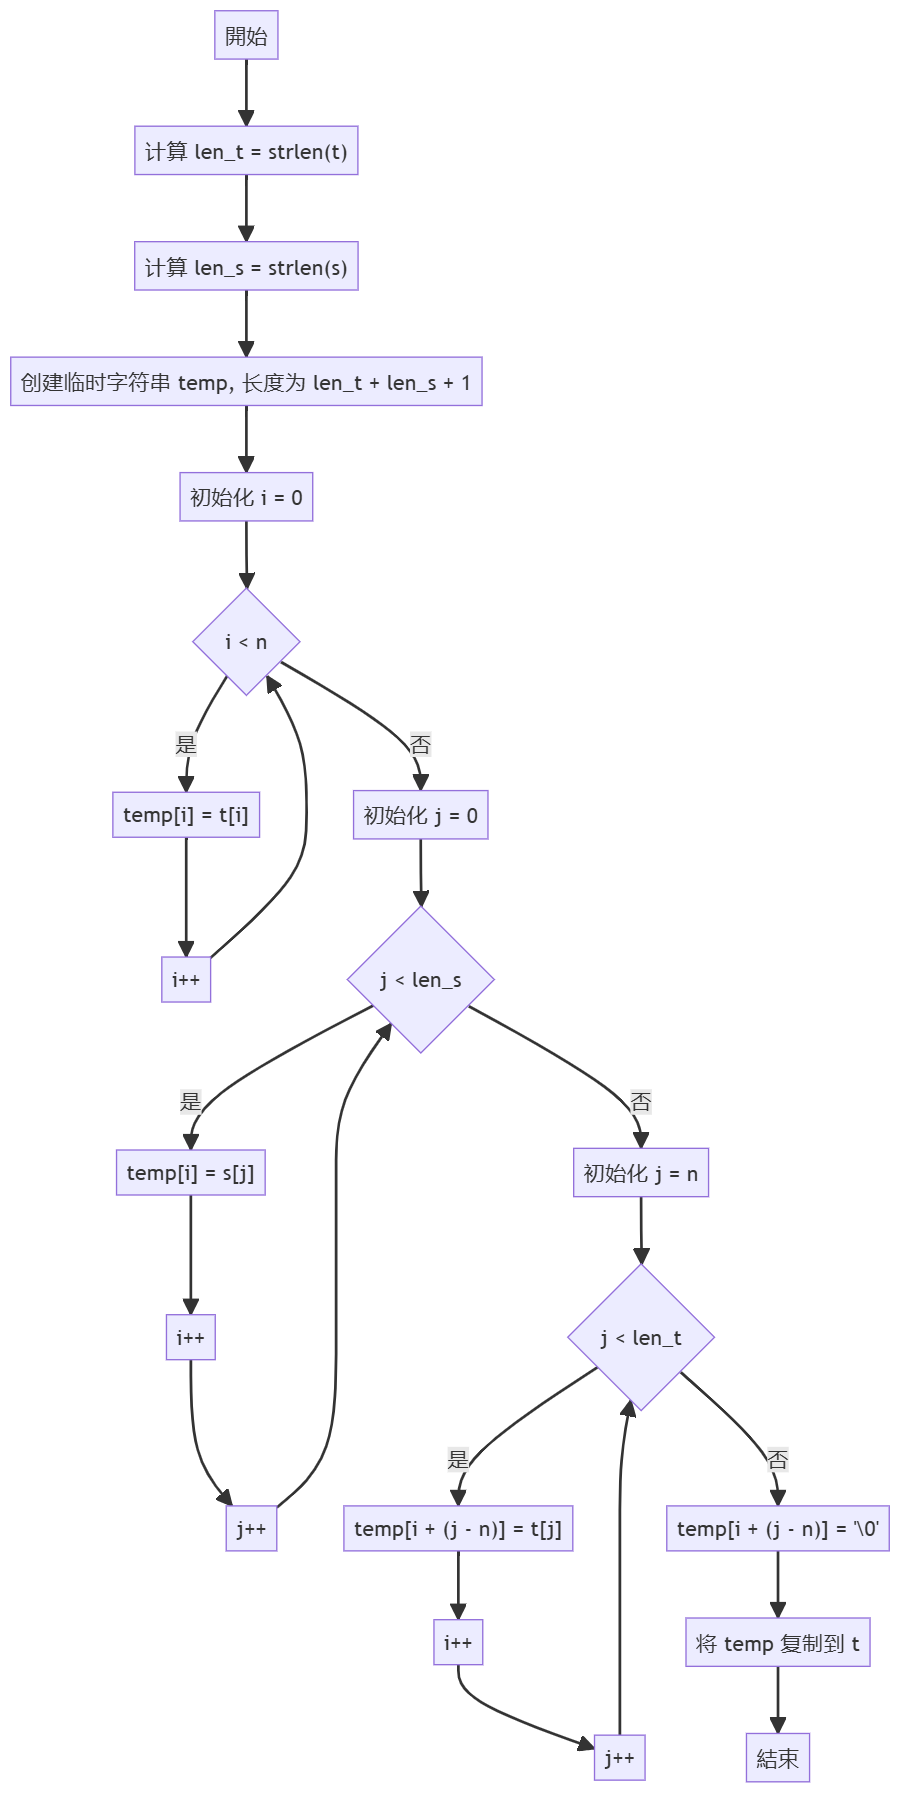
\includegraphics[scale=0.30]{images/5-9-2.png}
					\caption{流程图}
					\label{pic5-9-2}
				\end{center}
			\end{figure}
			
			
			\subsubsubsection{相关代码}
			相关代码(\ref{lst:5-9-1})：
			\begin{lstlisting}[style=commonCodeStyle, caption={示例}, label={lst:5-9-1}]
			#include <stdio.h>
			#include <stdlib.h>
			#include <string.h>
			void strnins(char t[], char s[], int n);
			int main() {
				char t[100], s[100];
				int n;
				scanf("%s", t);
				scanf("%s", s);
				scanf("%d", &n);
				strnins(t, s, n);
				printf("%s\n", t);
				return 0;
			}
			void strnins(char t[], char s[], int n) {
				int len_t = strlen(t);
				int len_s = strlen(s);
				int i, j;
				char temp[len_t + len_s + 1];
				for (i = 0; i < n; i++) {
					temp[i] = t[i];
				}
				for (j = 0; j < len_s; j++) {
					temp[i++] = s[j];
				}
				for (j = n; j < len_t; j++) {
					temp[i + (j - n)] = t[j];
				}
				temp[i + (j - n)] = '\0';
				strcpy(t, temp);
			}
			
			\end{lstlisting}
		
			\subsubsubsection{执行结果}
			执行结果(\ref{pic5-9-3})：
			\begin{figure}[H]
				\begin{center}
					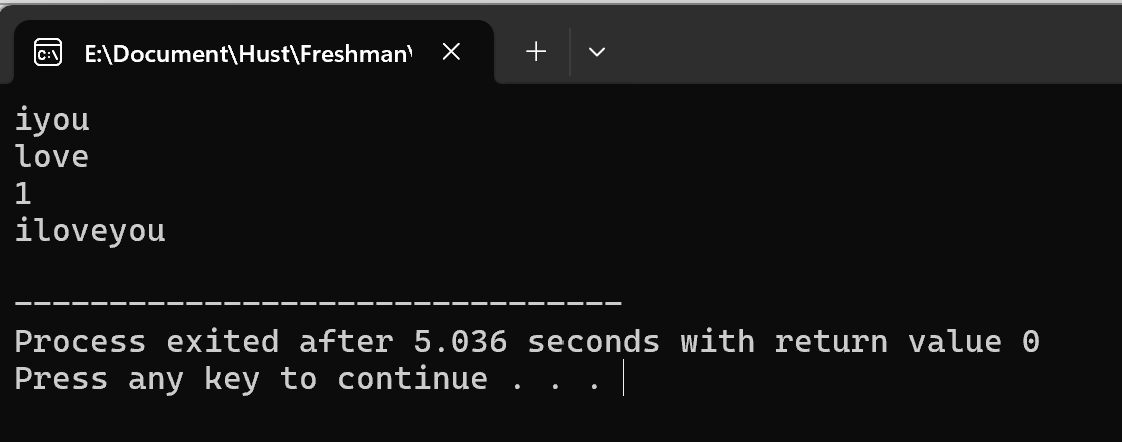
\includegraphics[scale=0.50]{images/5-9-3.png}
					\caption{执行结果}
					\label{pic5-9-3}
				\end{center}
			\end{figure}
			可见在原有字符串“iyou”上的第1位加插了字符串“love”，使其输出为“Iloveyou”
			
			\subsubsection{5-10 消除类游戏}
			\subsubsubsection{目标内容}
			消除类游戏是一种益智游戏，其核心规则是将一定的彼此相邻的相同元素配对消除。现给定一个n行m列的棋盘，棋盘中的每一个方格上放着一个棋子，每个棋子都有颜色，编号用1~9表示。当一行或一列上有连续3个或3个以上同色棋子时，这些棋子都被同时消除，对应的方格用0表示，请输出经过消除后的棋盘
			
			\subsubsubsection{分析}
			本题的流程图十分简洁，是一般最直接的输入->处理->输出，难在中间处理的部分。\\
			總流程圖(\ref{pic5-10-1})：
			\begin{figure}[H]
				\begin{center}
					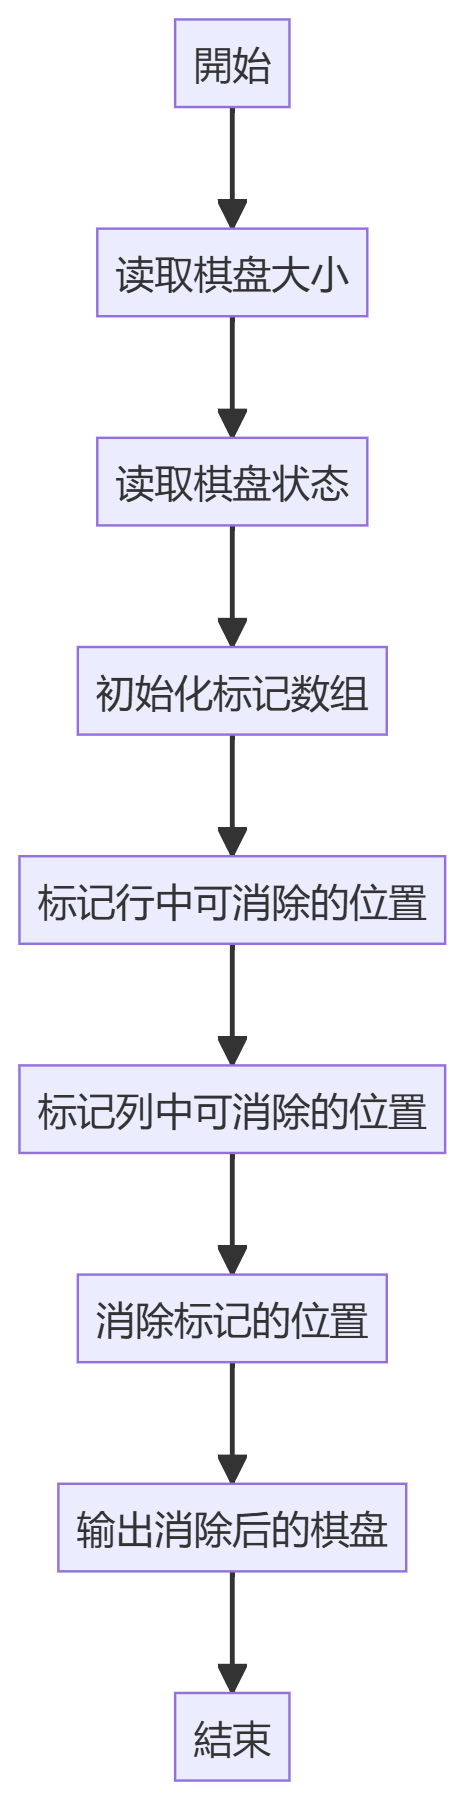
\includegraphics[scale=0.20]{images/5-10-1.png}
					\caption{總流程圖}
					\label{pic5-10-1}
				\end{center}
			\end{figure}
			
			     本题的核心在于识别棋盘上每行每列中连续出现 3 个或 3 个以上相同颜色（用 1 - 9 编号表示）的棋子，并将这些棋子消除，即将它们对应的方格标记为 0。这意味着需要逐行、逐列去检查棋子的颜色情况，判断是否满足消除条件。此题要构建这个棋盘，可利用二维数组int 标识符[n][m] 来表示棋盘\\
			設計思路：\\
			我们需要设计一个函数，该函数接收表示棋盘的二维数组 board、行数 n 和列数 m 作为参数，目的是对棋盘执行消除操作并返回消除后的棋盘状态。\\
			在函数内部，通过循环嵌套实现对棋盘的逐行、逐列遍历，先检查每行是否有满足消除条件的棋子，再检查每列是否有满足消除条件的棋子，每次检查到满足条件的区域就执行消除操作（将对应方格标记为 0）。\\
			由于消除部分棋子后可能会产生新的可消除区域，所以需要在一次完整的行、列遍历检查后，再次判断棋盘是否还有可消除的棋子，如果有则继续重复上述的检查和消除过程，直到棋盘上不再有可消除的棋子为止。\\
			这里处理矩阵时的代码比较复杂，主要可分为三部分：1.标记行中可消除的位置 2. 标记列中可消除的位置 3. 消除标记的位置
			相關流程圖(\ref{pic5-10-2}\ref{pic5-10-3})：
			\begin{figure}[H]
				\begin{center}
					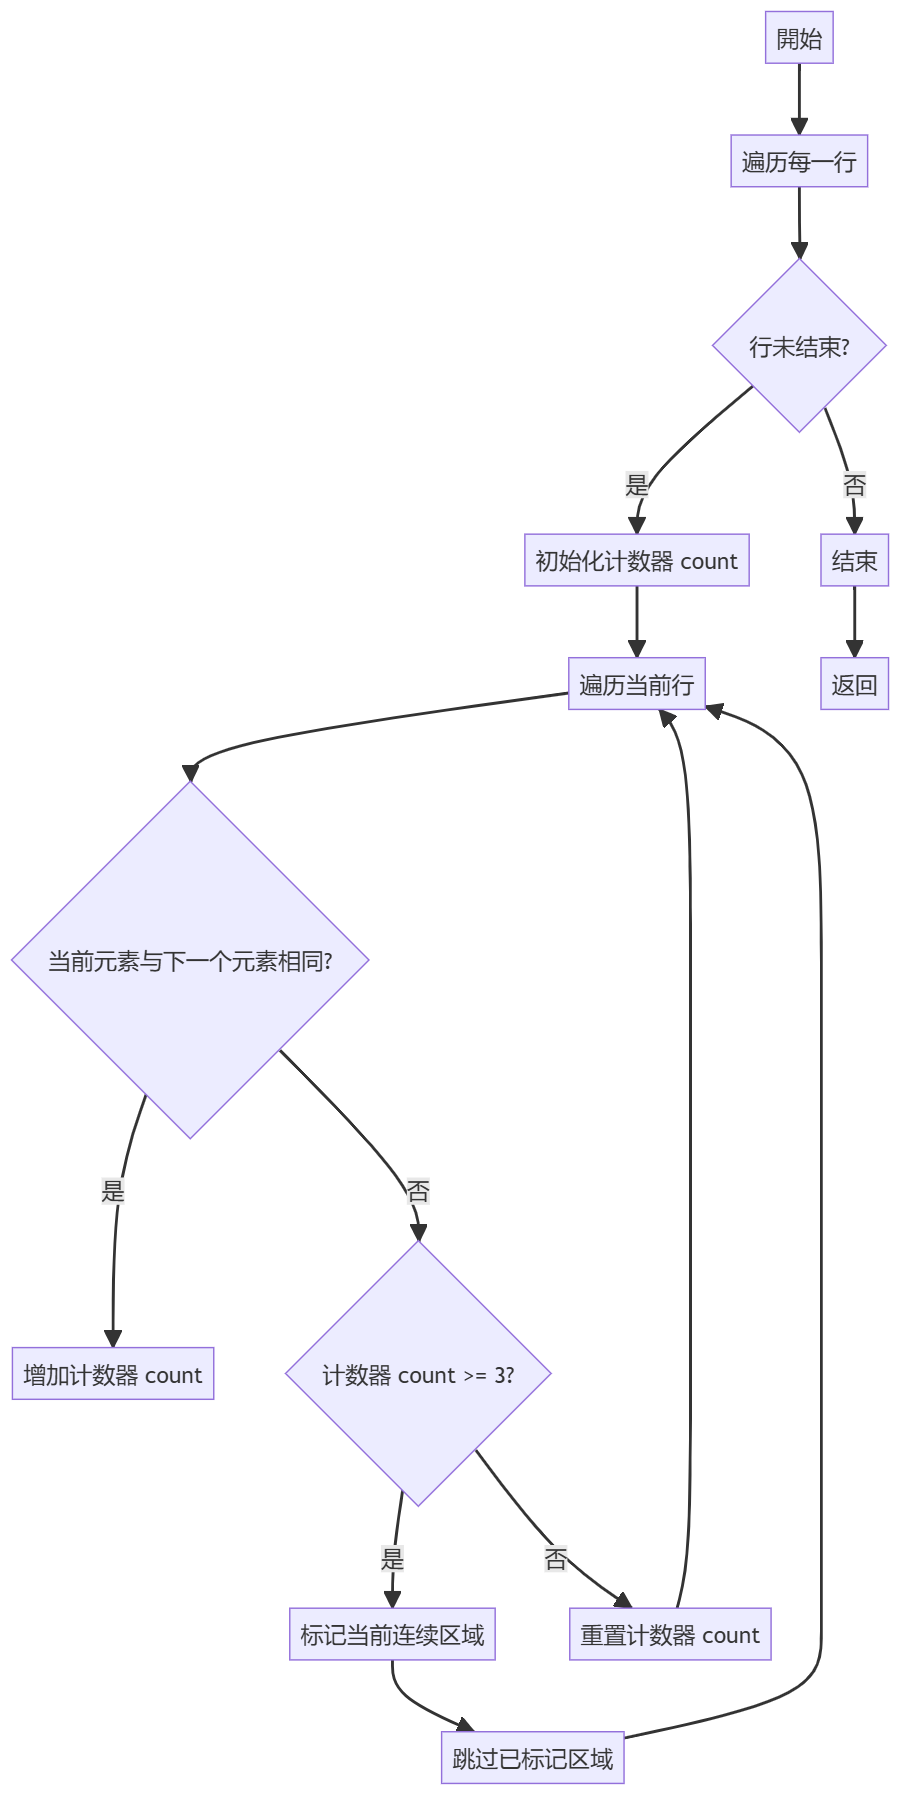
\includegraphics[scale=0.30]{images/5-10-2.png}
					\caption{流程圖}
					\label{pic5-10-2}
				\end{center}
			\end{figure}
		\begin{figure}[H]
			\begin{center}
				
\includegraphics[scale=0.30]{images/5-10-3.png}
				\caption{流程圖}
				\label{pic5-10-3}
			\end{center}
		\end{figure}
			
			\subsubsubsection{相关代码}
			相关代码(\ref{lst:5-10-1})：
			\begin{lstlisting}[style=commonCodeStyle, caption={示例}, label={lst:5-10-1}]
				#include <stdio.h>
				void markRowsToEliminate(int board[][100], int rows, int cols, int mark[][100]);
				void markColumnsToEliminate(int board[][100], int rows, int cols, int mark[][100]);
				void eliminateMarkedPositions(int board[][100], int rows, int cols, int mark[][100]);
				int main() {
					int board[100][100];
					int rows, cols;
					int i, j;
					scanf("%d %d", &rows, &cols);
					for (i = 0; i < rows; i++) {
						for (j = 0; j < cols; j++) {
							scanf("%d", &board[i][j]);
						}
					}
					int rowMark[100][100] = {0};
					int colMark[100][100] = {0};
					markRowsToEliminate(board, rows, cols, rowMark);
					markColumnsToEliminate(board, rows, cols, colMark);
					eliminateMarkedPositions(board, rows, cols, rowMark);
					eliminateMarkedPositions(board, rows, cols, colMark);
					for (i = 0; i < rows; i++) {
						for (j = 0; j < cols; j++) {
							printf("%d", board[i][j]);
							if (j < cols - 1) {
								printf(" ");
							}
						}
						printf("\n");
					}
					return 0;
				}
				void markRowsToEliminate(int board[][100], int rows, int cols, int mark[][100]) {
					int i, j, k;
					for (i = 0; i < rows; i++) {
						j = 0;
						while (j < cols) {
							int count = 1;
							k = j + 1;
							while (k < cols && board[i][k] == board[i][j]) {
								count++;
								k++;
							}
							if (count >= 3) {
								for (k = j; k < j + count; k++) {
									mark[i][k] = 1;
								}
							}
							j = k;
						}
					}
				}
				void markColumnsToEliminate(int board[][100], int rows, int cols, int mark[][100]) {
					int i, j, k;
					for (j = 0; j < cols; j++) {
						i = 0;
						while (i < rows) {
							int count = 1;
							k = i + 1;
							while (k < rows && board[k][j] == board[i][j]) {
								count++;
								k++;
							}
							if (count >= 3) {
								for (k = i; k < i + count; k++) {
									mark[k][j] = 1;
								}
							}
							i = k;
						}
					}
				}
				void eliminateMarkedPositions(int board[][100], int rows, int cols, int mark[][100]) {
					int i, j;
					for (i = 0; i < rows; i++) {
						for (j = 0; j < cols; j++) {
							if (mark[i][j] == 1) {
								board[i][j] = 0;
							}
						}
					}
				}
			\end{lstlisting}
			
			\subsubsubsection{执行结果}
			执行结果(\ref{pic5-10-4}\ref{pic5-10-5})：
			\begin{figure}[H]
				\begin{center}
					
\includegraphics[scale=0.50]{images/5-10-4.png}
					\caption{执行示例}
					\label{pic5-10-4}
				\end{center}
			\end{figure}
			\begin{figure}[H]
			\begin{center}
				
\includegraphics[scale=0.50]{images/5-10-5.png}
				\caption{执行示例}
				\label{pic5-10-5}
			\end{center}
			\end{figure}
			可以见到代码也是成功被执行的，能够实现矩阵的消除，通过遍历的过作去完成，先对位置标记再进行消除操作是十分关键的，之前自己刚开始写的时候没写好主要就是因为太急消除，这时候会阻碍了行(列)的消除，使得输出结果有误。因此，在编程时是十分注重程序的执行顺序和思想的。
\newpage
			\subsubsection{5-11 N阶顺转方阵}
			\subsubsubsection{目标内容}
			本关任务：将1、2、3、…、n*n 从左上角开始，由外层至中心按顺时针方向螺旋排列所形成的数字方阵，成为n阶顺转方阵，5阶顺转方阵如下方数字阵列所示。编写程序，读入n，构造并输出n阶顺转方阵。
			\subsubsubsection{分析}
			这段 C 语言代码实现生成并输出 n 阶顺转方阵的功能。在 main 函数里获取用户输入的 n 值，调用 void函数按顺时针螺旋方式将 1 到 n² 的数字填充进二维数组 matrix，利用边界变量控制填充顺序，每填充完一层对应边界变量调整，循环直至填完所有数字。之后通过 void定义的函数将生成好的方阵以矩阵格式输出展示，整体完成按要求构造并输出 n 阶顺转方阵的任务。\\
			总流程图(\ref{pic5-11-1})：
			\begin{figure}[H]
				\begin{center}
					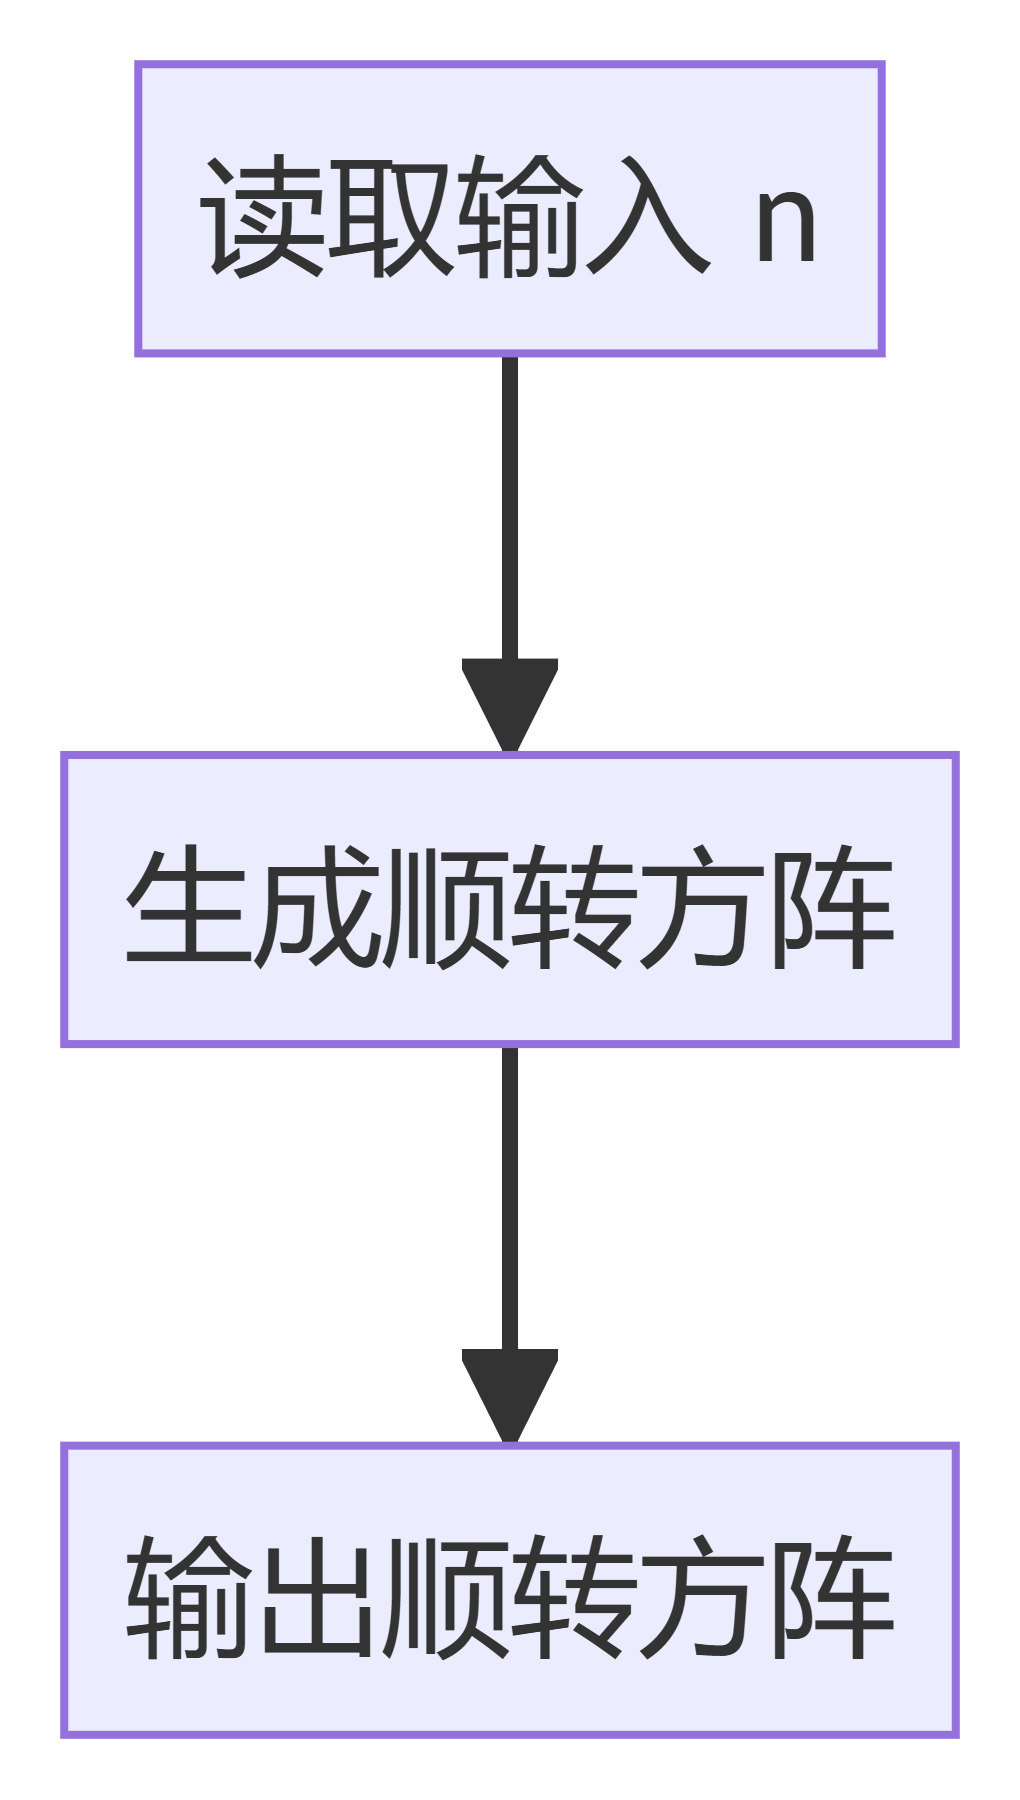
\includegraphics[scale=0.10]{images/5-11-1.png}
					\caption{总流程图}
					\label{pic5-11-1}
				\end{center}
			\end{figure}
			設計思路：\\
			本题整体采用模块化设计，在主函数中先定义变量接收用户输入的方阵阶数 n 及用于存储方阵的二维数组，接着调用生成方阵的函数，按顺时针螺旋方式，利用边界变量控制，从外层到内层逐次填充 1 到 n² 的数字到数组，每填充完一层相应调整边界变量，直至填满。之后调用输出函数，通过两层嵌套循环遍历数组，输出各元素并按需添加空格和换行，将生成好的 n 阶顺转方阵展示出来，以此实现构造并输出 n 阶顺转方阵的功能。
			流程图(\ref{pic5-11-2})：
			\begin{figure}[H]
				\begin{center}
					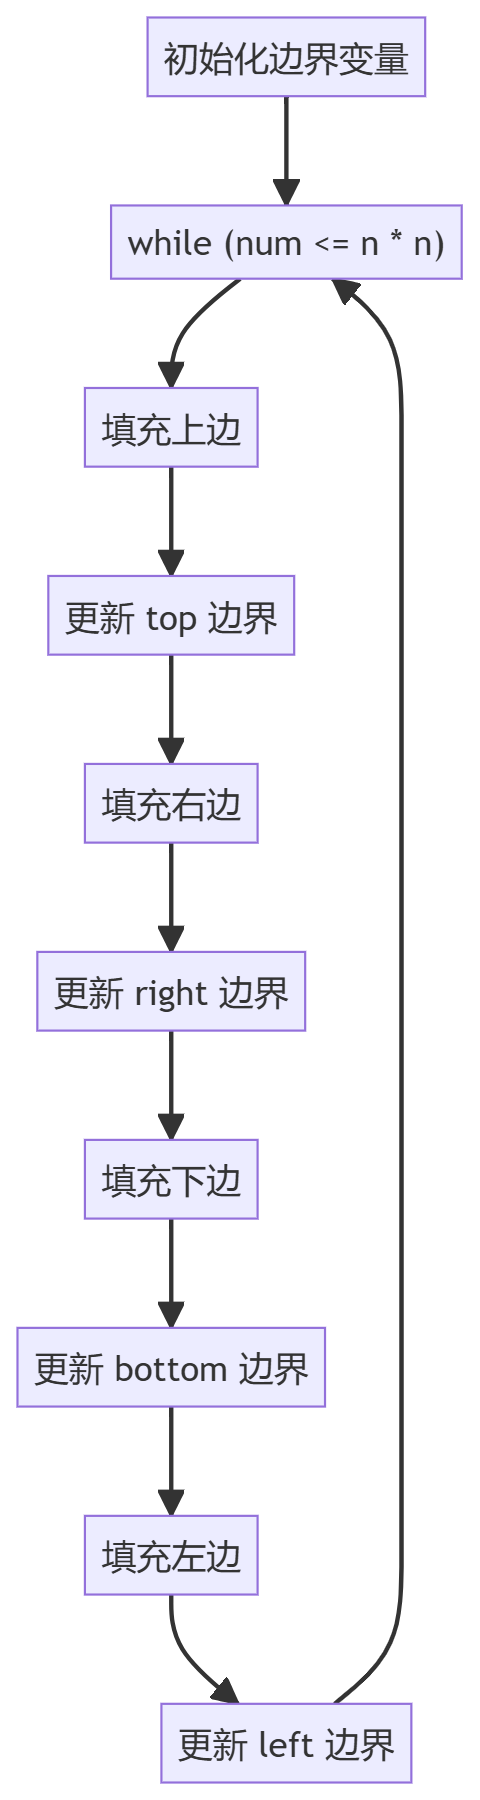
\includegraphics[scale=0.20]{images/5-11-2.png}
					\caption{流程图}
					\label{pic5-11-2}
				\end{center}
			\end{figure}
			
			\subsubsubsection{相关代码}
			相关代码(\ref{lst:5-11-1})：
			\begin{lstlisting}[style=commonCodeStyle, caption={示例}, label={lst:5-11-1}]
				#include <stdio.h>
				#include <stdlib.h>
				void generateSpiralMatrix(int n, int matrix[][100]);
				void printMatrix(int n, int matrix[][100]);
				int main() {
					int n;
					int matrix[100][100];
					scanf("%d", &n);
					generateSpiralMatrix(n, matrix);  
					printMatrix(n, matrix);
					return 0;
				}
				void generateSpiralMatrix(int n, int matrix[][100]) {
					int top = 0, bottom = n - 1, left = 0, right = n - 1;
					int num = 1;
					while (num <= n * n) {
						for (int i = left; i <= right; i++) {
							matrix[top][i] = num++;
						}
						top++;
						for (int i = top; i <= bottom; i++) {
							matrix[i][right] = num++;
						}
						right--;
						for (int i = right; i >= left; i--) {
							matrix[bottom][i] = num++;
						}
						bottom--;
						for (int i = bottom; i >= top; i--) {
							matrix[i][left] = num++;
						}
						left++;
					}
				}
				void printMatrix(int n, int matrix[][100]) {
					for (int i = 0; i < n; i++) {
						for (int j = 0; j < n; j++) {
							printf("%d", matrix[i][j]);
							if (j < n - 1) {
								printf(" ");
							}
						}
						printf("\n");
					}
				}
			\end{lstlisting}
			
			\subsubsubsection{执行结果}
			执行结果(\ref{pic5-11-3}\ref{pic5-11-4})：
			\begin{figure}[H]
				\begin{center}
					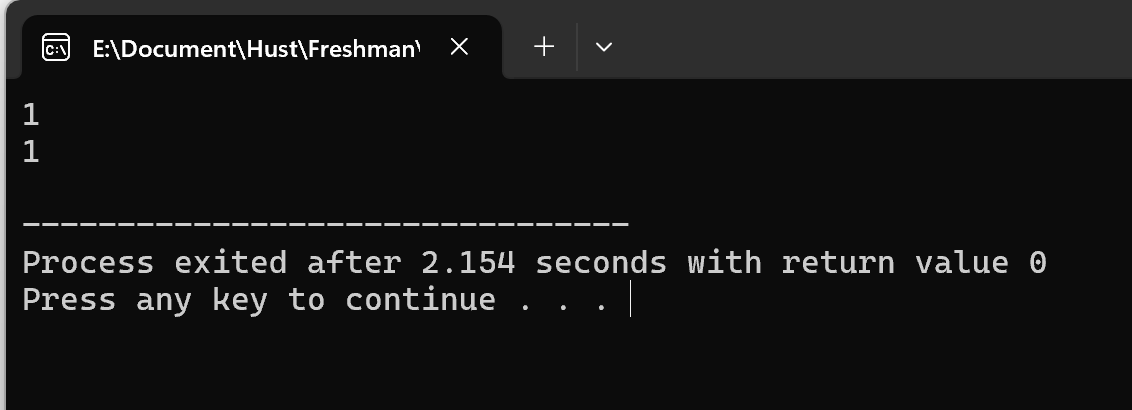
\includegraphics[scale=0.70]{images/5-11-3.png}
					\caption{执行示例}
					\label{pic5-11-3}
				\end{center}
			\end{figure}
			\begin{figure}[H]
			\begin{center}
				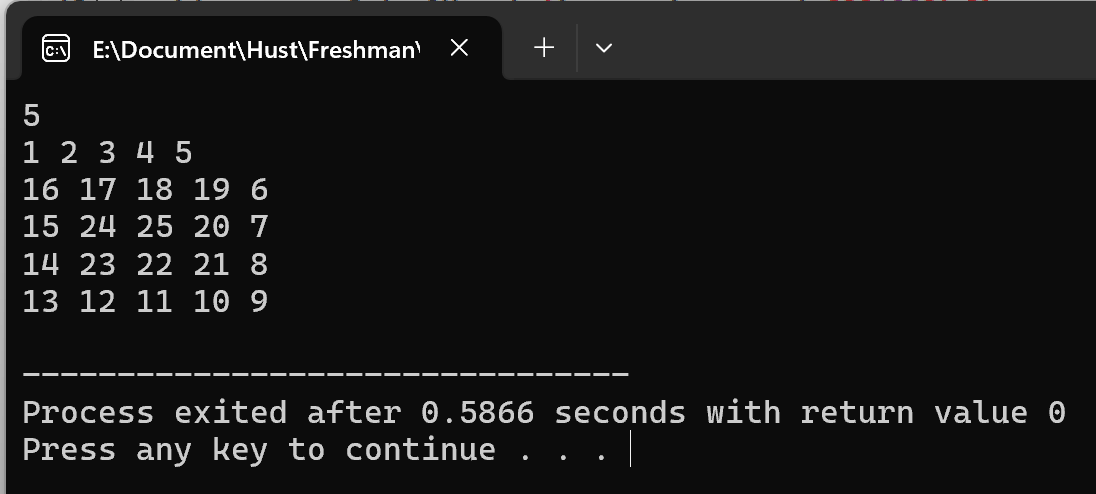
\includegraphics[scale=0.70]{images/5-11-4.png}
				\caption{执行示例}
				\label{pic5-11-4}
			\end{center}
			\end{figure}
		由此可见该程序能够成功输出N阶顺转矩阵。\\
		填充上侧一行：\\
		使用一个 for 循环，从左边界 left 到右边界 right 遍历，将当前的数字 num 依次填充到 matrix[top][i] 中（其中 i 为循环变量），每填充一个位置，num 的值就自增 1，代表下一个要填充的数字。完成这一行的填充后，将上边界 top 的值加 1，准备填充下一层的右侧一列。\\
		填充右侧一列：\\
		接着再用一个 for 循环，从上边界 top 到下边界 bottom 遍历，把 num 依次填充到 matrix[i][right] 中，同样每填充一次 num 自增 1，填充完这一列后，将右边界 right 的值减 1，以便后续填充下一层的下侧一行。
		\\填充下侧一行：\\
		然后通过一个 for 循环，从右边界 right 到左边界 left 反向遍历，将 num 填充到 matrix[bottom][i] 中（注意这里 i 是反向变化的），num 持续自增，填充完这一行后，下边界 bottom 的值减 1，为填充下一层的左侧一列做准备。
		\\填充左侧一列：\\
		最后利用一个 for 循环，从下边界 bottom 到上边界 top 反向遍历，把 num 填充到 matrix[i][left] 中，num 继续自增，填充完这一列后，左边界 left 的值加 1，至此完成一层的填充，进入下一轮 while 循环，重复上述步骤填充下一层，直到整个方阵所有位置都填充完毕。
		通过两层嵌套的 for 循环来遍历二维数组 matrix，外层循环控制行索引，内层循环控制列索引。对于每个元素 matrix[i][j]，先使用 printf 函数输出其数值，然后通过判断 j < n - 1 来确定是否为该行的最后一个元素，如果不是，则输出一个空格进行分隔，使得每行元素之间有合适的间隔。当内层循环结束，也就是一行元素都输出完后，使用 printf 函数输出换行符 \n，开始下一行元素的输出，如此循环，直至整个方阵的所有元素都被输出，让用户能直观地看到生成的顺转方阵的样子。
		
			
			\subsubsection{5-12 迷宫问题}
			\subsubsubsection{目标内容}
			迷宫问题。编程找出从入口（左上角方格）经过迷宫到达出口（右下角方格）的所有路径，迷宫问题示意如下方数字阵列所示，0所表示的地方是不可以通行的，只能从1走到与它相邻（四邻域：上、下、左、右相邻）的1上，且不能走重复路径。
			\subsubsubsection{分析}
			要解决迷宫问题，即找出从迷宫入口（左上角方格）到出口（右下角方格）的所有可行路径。迷宫用二维数组表示，其中 0 代表不可通行区域，1 代表可通行区域。代码通过深度优先搜索（DFS）算法来遍历迷宫，记录下每条从入口到出口的路径，并输出这些路径\\
			总流程图(\ref{pic5-12-1})：\\
			\begin{figure}[H]
				\begin{center}
					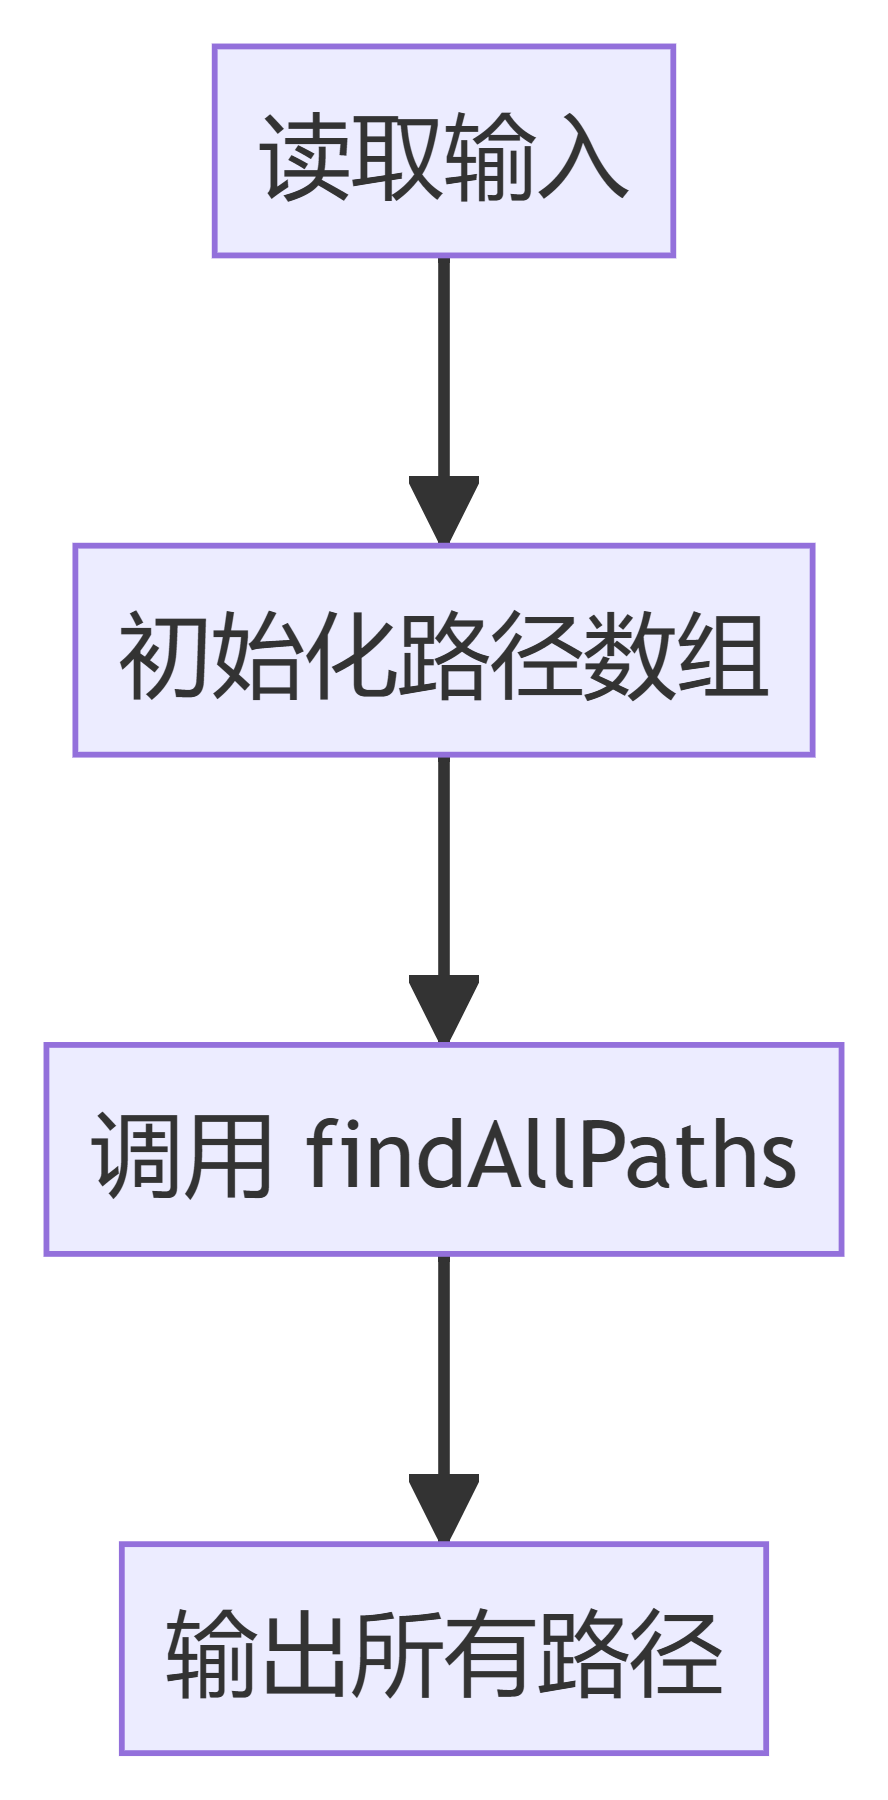
\includegraphics[scale=0.10]{images/5-12-1.png}
					\caption{总流程图}
					\label{pic5-12-1}
				\end{center}
			\end{figure}
			
			設計思路：\\
			首先我们要创建一个同样大小的二维数组 path，初始化为 0。定义起点 start 和终点 end。调用 dfs 函数从起点开始进行深度优先搜索。\\
			这里说明一下核心DFS算法的设计思路\\
			DFS（深度优先搜索）函数设计思路：\\
			首先进行边界和可行性判断，如果当前位置超出迷宫范围（通过坐标与行数、列数比较判断）、当前位置是不可通行的（maze[current.x][current.y] == 0）或者已经走过（path[current.x][current.y] == 1），则直接返回，不再继续探索该位置。\\
			若当前位置合法且可通行，将当前位置在 path 数组中标记为 1，表示已走过。接着判断当前位置是否就是终点，如果是，则说明找到了一条从入口到出口的路径，此时路径数量 pathCount 加 1，输出路径编号以及通过调用 printPath 函数输出该条路径的具体情况（用 1 和 0 展示走过和未走过的方格），然后将当前位置标记回 0（回溯操作，方便后续探索其他路径时该位置能被再次访问），并返回。\\
			如果当前位置不是终点，就分别向当前位置的上、下、左、右四个方向（通过创建对应方向的 Point 结构体来表示新位置）进行递归调用 dfs 函数，继续深度优先搜索，探索从这些相邻位置能否到达终点，每探索完一个方向后，同样进行回溯操作（将当前位置标记为 0），确保能遍历所有可能的路径情况。\\
			相關流程圖(\ref{pic5-12-2})：
			\begin{figure}[H]
				\begin{center}
					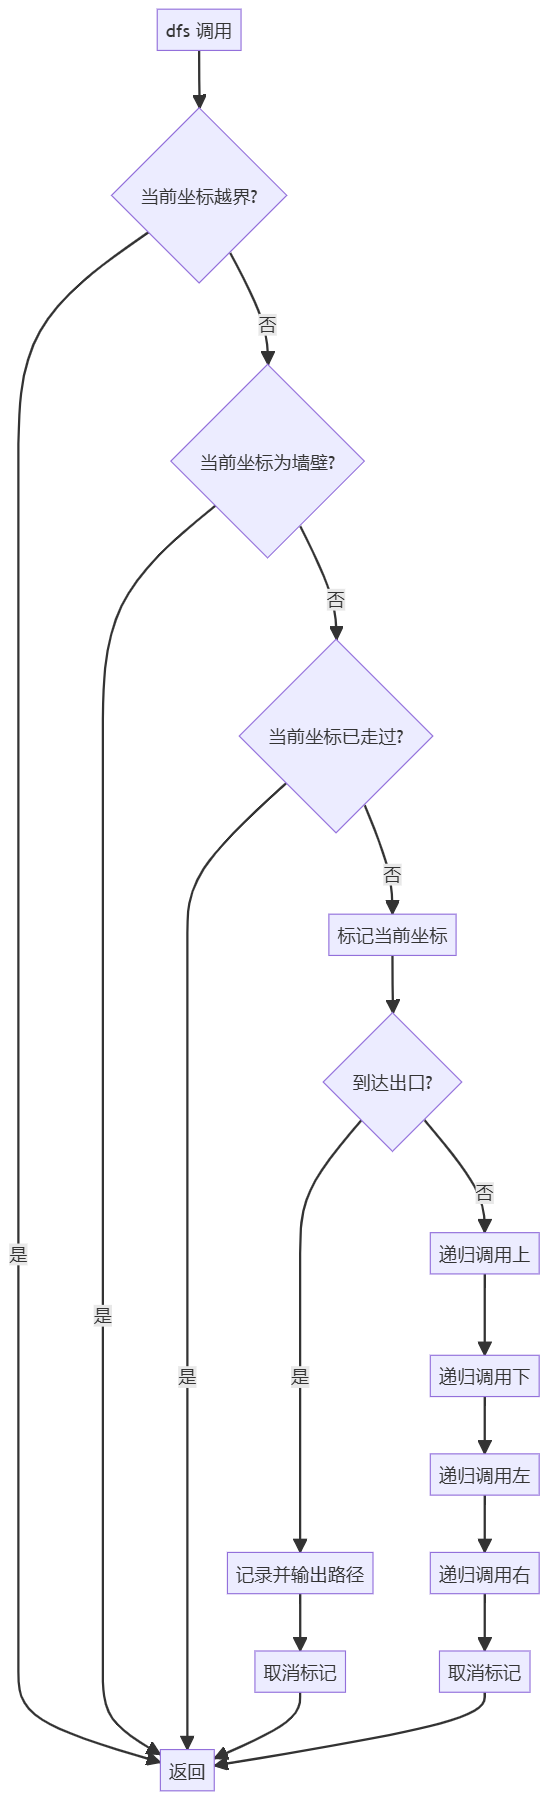
\includegraphics[scale=0.30]{images/5-12-2.png}
					\caption{流程图}
					\label{pic5-12-2}
				\end{center}
			\end{figure}
			
			\subsubsubsection{相关代码}
			相关代码(\ref{lst:5-12-1})：
			\begin{lstlisting}[style=commonCodeStyle, caption={示例}, label={lst:5-12-1}]
				#include <stdio.h>
				#include <stdlib.h>
				#define MAX_ROWS 100
				#define MAX_COLS 100
				typedef struct {
					int x;
					int y;
				} Point;
				int pathCount = 0;
				void findAllPaths(int maze[MAX_ROWS][MAX_COLS], int rows, int cols);
				void printPath(int path[MAX_ROWS][MAX_COLS], int rows, int cols);
				void dfs(int maze[MAX_ROWS][MAX_COLS], int path[MAX_ROWS][MAX_COLS], Point current, Point end, int rows, int cols);
				int main() {
					int maze[MAX_ROWS][MAX_COLS];
					int rows, cols;
					int i, j;
					scanf("%d %d", &rows, &cols);
					for (i = 0; i < rows; i++) {
						for (j = 0; j < cols; j++) {
							scanf("%d", &maze[i][j]);
						}
					}
					findAllPaths(maze, rows, cols);
					return 0;
				}
				void findAllPaths(int maze[MAX_ROWS][MAX_COLS], int rows, int cols) {
					int path[MAX_ROWS][MAX_COLS];
					Point start = {0, 0};
					Point end = {rows - 1, cols - 1};
					for (int i = 0; i < rows; i++) {
						for (int j = 0; j < cols; j++) {
							path[i][j] = 0;
						}
					}
					dfs(maze, path, start, end, rows, cols);
				}
				void dfs(int maze[MAX_ROWS][MAX_COLS], int path[MAX_ROWS][MAX_COLS], Point current, Point end, int rows, int cols) {
					if (current.x < 0 || current.x >= rows || current.y < 0 || current.y >= cols ||
					maze[current.x][current.y] == 0 || path[current.x][current.y] == 1) {
						return;
					}
					path[current.x][current.y] = 1;
					if (current.x == end.x && current.y == end.y) {
						pathCount++;
						printf("%d\n", pathCount);
						printPath(path, rows, cols);
						path[current.x][current.y] = 0;
						return;
					}
					Point up = {current.x - 1, current.y};
					dfs(maze, path, up, end, rows, cols);
					Point down = {current.x + 1, current.y};
					dfs(maze, path, down, end, rows, cols);
					Point left = {current.x, current.y - 1};
					dfs(maze, path, left, end, rows, cols);
					Point right = {current.x, current.y + 1};
					dfs(maze, path, right, end, rows, cols);
					path[current.x][current.y] = 0;
				}
				void printPath(int path[MAX_ROWS][MAX_COLS], int rows, int cols) {
					for (int i = 0; i < rows; i++) {
						for (int j = 0; j < cols; j++) {
							printf("%d", path[i][j]);
							if (j < cols - 1) {
								printf(" ");
							}
						}
						printf("\n");
					}
				}
				
			\end{lstlisting}
			
			\subsubsubsection{执行结果}
			执行结果(\ref{pic5-12-3})：
		\begin{figure}[H]
			\begin{center}
				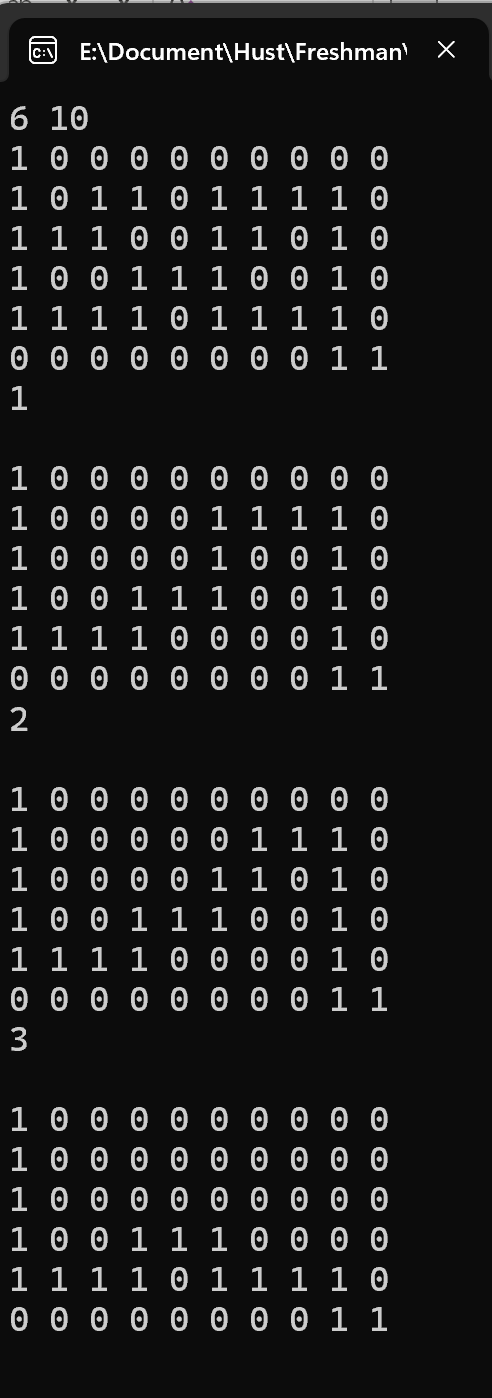
\includegraphics[scale=0.70]{images/5-12-3.png}
				\caption{执行示例}
				\label{pic5-12-3}
			\end{center}
		\end{figure}
			首先需要把迷宫抽象成二维数组的形式，用 0 和 1 来清晰地表示不可通行区域和可通行区域，这一步骤是后续进行算法设计和代码编写的基础。将现实问题转化为计算机能够处理的数据结构，让整个问题变得更有条理，便于操作和思考解决办法。\\
			明确了起点和终点的坐标表示，进一步把寻找路径的问题聚焦到如何从给定的起点出发，通过合理的探索规则去尝试抵达终点，这种明确的问题定义和模型建立有助于确定具体的解题方向。\\
			DFS 是一种用于遍历或搜索图（在迷宫问题里可以把迷宫看作是一种特殊的图结构，方格就是节点，相邻方格之间的可通行关系就是边）、树等数据结构的算法。它的核心思想是沿着一条路径尽可能深地探索下去，直到无法继续前进（比如遇到边界、不符合条件的节点或者已经访问过的节点等情况），然后回溯到上一个未完全探索的节点，再继续沿着另一条未探索的分支路径深入，如此反复，直到遍历完所有可能的路径。\\
			这种思路能够暴力破解问题，但同时所需要的运行时间亦是巨大的，因此掌握熟练多种算法的思路往往是必不可少的。
			
		\subsection{实验五小結}
		在完成诸多关于数组的实验题过程中，我不仅对数组这一基础数据结构有了更深入透彻的理解与掌握，还接触并运用到了大量数组以外的知识和算法，极大地拓宽了我的编程视野与思维方式。以下是我对此次数组实验题学习经历的详细总结与深刻反思。
		\subsubsection{知识与技能提升}
		（一）数组基础的巩固与深化\\
		数组作为一种存储相同类型数据的线性数据结构，在实验题中频繁出现，使我对其特性和操作有了更熟练的运用。通过对数组元素的访问、修改、遍历等基本操作的大量实践，我深刻理解了数组下标与内存地址之间的对应关系，明白了如何通过合理运用下标来高效地操作数组中的数据。例如，在处理一些涉及数据统计和筛选的问题时，能够灵活地运用循环结构和数组下标，快速定位并处理目标元素，提高了程序的执行效率。\\
		（二）与其他数据结构的关联与拓展\\
		在部分实验题中，数组与其他数据结构（如结构体）相互结合使用，展现出了更强大的数据组织和处理能力。例如，通过定义结构体数组来存储具有多个属性的数据对象，不仅可以方便地对每个对象的各个属性进行单独操作，还能够以数组的形式对一组相关对象进行整体处理。这种结合方式使我认识到不同数据结构之间并非孤立存在，而是可以相互协作，共同解决复杂的编程问题。在处理涉及多个相关数据实体且需要批量处理的场景时，这种数据结构的组合应用尤为重要，它让我学会从更宏观的角度去思考数据的组织和管理，提升了我构建复杂数据模型的能力。\\
		（三）算法在数组中的应用\\
		实验题中广泛涉及各种算法在数组上的应用，如排序算法（冒泡排序、选择排序、快速排序等）、查找算法（线性查找、二分查找等）以及遍历算法（深度优先遍历、广度优先遍历的变体等）。这些算法的应用让我明白了如何根据具体问题的需求选择合适的算法策略来对数组数据进行处理，以达到优化程序性能的目的。
		排序算法：在处理数组排序问题时，我深入学习了不同排序算法的原理和实现方式。冒泡排序虽然简单易懂，但时间复杂度较高，适用于小规模数据的排序；而快速排序则采用了分治思想，通过选择一个基准元素将数组分为两部分，递归地对两部分进行排序，平均时间复杂度较低，在处理大规模数据时表现出色。通过对这些排序算法的实践，我不仅能够根据数据规模和实际需求选择最合适的排序方法，还学会了对排序算法进行简单的优化，如在冒泡排序中加入标记位来提前结束排序过程，或者在快速排序中合理选择基准元素以避免最坏情况的发生。这些优化技巧不仅提高了程序的运行效率，也培养了我在编程过程中不断追求性能提升的意识。
		查找算法：对于数组查找问题，线性查找适用于无序数组，但时间复杂度为 ；二分查找则要求数组必须有序，但其时间复杂度可降低至 。在实际应用中，我学会了根据数组的有序性和查找需求来选择合适的查找算法。例如，在处理频繁查找操作且数组相对稳定不变的情况下，先对数组进行排序，然后使用二分查找可以大大提高查找效率。此外，我还了解到一些基于哈希表的查找算法，它们在特定场景下能够实现更快速的查找操作，但需要额外的空间来存储哈希表。通过对这些查找算法的学习和实践，我深刻认识到在编程中权衡时间和空间复杂度的重要性，以及根据具体问题场景选择最优算法策略的必要性。
		遍历算法：在涉及数组元素的遍历和搜索场景中，我运用了深度优先遍历和广度优先遍历的思想。例如，在处理二维数组表示的迷宫问题时，通过深度优先遍历算法来探索从起点到终点的所有可能路径，利用递归函数来实现深度优先遍历的过程，同时通过标记已访问的数组元素来避免重复访问，提高算法效率。而在一些需要按照层次顺序处理数组元素的问题中，如树状结构的层次遍历模拟题，我则运用了广度优先遍历的思想，借助队列数据结构来实现元素的层次顺序访问。这些遍历算法的应用让我更加熟练地掌握了递归和队列等编程技术，同时也培养了我在面对不同问题场景时灵活选择合适算法策略的能力。
		\subsubsection{问题解决的思路多样化}
		（一）复杂问题的分析与拆解\\
		面对实验题中那些较为复杂的问题，我逐渐学会了运用分析和拆解的方法将其转化为一系列可管理和解决的子问题。例如，在处理涉及多个条件限制和多种数据处理步骤的数组问题时，我首先会仔细梳理问题的需求和给定的条件，确定问题的关键目标和核心难点。然后，将整个问题按照功能模块或数据处理流程拆分成若干个相对独立的子问题，每个子问题专注于完成特定的任务或处理特定部分的数据。这种分析和拆解的思维方式使我在面对复杂编程问题时不再感到无从下手，而是能够有条不紊地逐步推进解决方案的设计和实现。通过将大问题分解为小问题，我不仅降低了问题的解决难度，还提高了代码的可读性和可维护性，因为每个子问题的解决代码相对独立且功能明确，便于后续的调试和修改。\\
		（二）逻辑思维与编程思维的强化\\
		在解决数组实验题的过程中，我的逻辑思维和编程思维得到了极大的锻炼和强化。每一道实验题都像是一个逻辑谜题，需要我运用严谨的逻辑推理来设计合理的算法和数据处理流程。在编写代码之前，我会先在脑海中构建出问题的解决方案框架，考虑各种可能的情况和边界条件，并设计相应的应对策略。这种逻辑思考和规划的过程让我学会了从抽象的问题描述逐步转化为具体的编程实现步骤，培养了我结构化编程的思维方式。同时，在代码编写过程中，我需要不断地调试和优化代码，以确保程序的正确性和高效性。这一过程锻炼了我发现问题、定位问题和解决问题的能力，使我能够更加敏锐地察觉到代码中的逻辑错误和潜在的性能瓶颈，并通过合理的代码调整和算法优化来加以解决。通过反复的实践和积累，我的逻辑思维和编程思维逐渐变得更加严谨、灵活和高效，能够更好地应对各种复杂编程任务的挑战。\\
		（三）调试技巧与错误处理能力的提升\\
		调试是编程过程中不可或缺的重要环节，在数组实验题的实践中，我积累了丰富的调试技巧和错误处理经验。当程序出现错误或异常结果时，我学会了首先仔细观察程序的输出和运行时的表现，通过分析错误信息和程序的执行流程来初步定位问题可能出现的区域。然后，我会运用调试工具（如断点调试、变量监视等）来深入检查程序在关键位置的变量值和执行状态，逐步缩小问题的范围，直至找到错误的根源。在处理数组相关的错误时，常见的问题包括数组下标越界、数组初始化错误、算法逻辑错误导致的数组元素处理不当等。针对这些问题，我学会了在编写代码时加入必要的边界检查和错误处理机制，以提高程序的健壮性。例如，在访问数组元素之前，先检查下标是否在合法范围内；在进行数组排序或查找操作时，确保数组不为空且满足相应的前提条件。通过不断地调试和优化程序，我不仅能够更加熟练地运用调试工具和技巧，还培养了良好的错误预防和处理意识，使我编写的程序能够更加稳定可靠地运行。
		\subsubsection{心得与感悟}
		通过大量数组实验题的练习，我深刻体会到编程是一门需要不断实践才能真正掌握的艺术。理论知识固然重要，但只有通过实际动手编写代码，将所学的知识应用到具体的问题解决中，才能真正理解和内化这些知识。在实践过程中，我遇到了各种各样的问题和挑战，每一次解决问题的过程都是一次学习和成长的机会。从最初的对一些简单数组操作的生疏和错误频出，到后来能够熟练运用数组及相关知识解决复杂的编程问题，这种能力的提升离不开大量的实践积累。编程不仅仅是按照语法规则编写代码，更是一种创造性的活动，需要在实践中不断尝试新的算法策略、优化代码结构、提高程序性能，才能编写出高质量、高效率的程序代码。\\
		只有不断学习，才能进步，只有不断实践，才能运用自如。
		
	\section{实验七 结构与联合}
		\subsection{程序改错与跟踪调试}
			\subsubsection{7-1 表达式求值的程序验证}
			\subsubsubsection{目标内容}
			设有下面说明,请先自己计算表7-1中表达式的值,然后通过编程计算来加以验证。各表达式之间相互无关\\
			需要验证的相关程序(\ref{lst:7-1-1})：
			\begin{lstlisting}[style=commonCodeStyle, caption={示例}, label={lst:7-1-1}]
				#include<stdio.h>
				#include<stdlib.h>
				char u[]="UVWXYZ",v[]="xyz";
				struct T{
					int x;
					char c;
					char *t;
				}a[]={{11,'A',u},{100,'B',v}},*p=a;
				int main()
				{
					int n;
					scanf("%d",&n);
					switch (n){
						case 1:
						printf("%d",(++p)->x);
						break;
						case 2:
						p++;
						printf("%c",p->c);   
						break;
						case 3:
						p++;
						printf("%c",*p->t);
						break;        
						case 4:
						printf("%c",*(++p)->t);
						break;
						case 5:
						printf("%c",*++p->t);
						break;
						case 6:
						printf("%c",++*p->t);
						break;    
					}
					return 0;
				}
			\end{lstlisting}
			\subsubsubsection{分析}
			对不同分模功能说明：\\
			Case1\\
			在这个 case 中，执行了 (++p)->x 操作。++p 会使指针 p 自增，也就是让 p 指向结构体数组 a 的下一个元素，即 a[1]。然后通过 -> 运算符访问 p 所指向结构体（此时是 a[1]）的成员 x，并将其值输出。由于 a[1].x 的值初始化为 100，所以此 case 执行后会输出 100。\\
			Case2\\
			首先执行 p++，同样使指针 p 指向下一个结构体元素（也就是 a[1]），这和 case 1 中指针 p 的最终指向是一样的。然后通过 p->c 访问 p 所指向结构体（a[1]）的成员 c，并输出该字符值。因为 a[1].c 的值为 'B'，所以此 case 执行后会输出 'B'。\\
			Case3\\
			先是 p++，让 p 指向 a[1]。然后 *p->t 这个表达式的运算顺序是先通过 p->t 获取 p 所指向结构体（即 a[1]）中成员 t 的值，此时 p->t 指向字符数组 v（因为 a[1].t 指向 v），再对这个指针进行解引用 *，就会获取到 v 数组的第一个字符，也就是 'x'，所以此 case 执行后会输出 'x'。\\
			Case4\\
			这里先执行 (++p)->t，++p 使 p 指向 a[1]，然后获取 a[1].t，也就是指向字符数组 v 的指针。接着再对这个指针进行解引用 *，同样获取到 v 数组的第一个字符 'x'，所以此 case 执行后输出 'x'，和 case 3 的输出结果一样，不过这里是先对指针 p 进行自增操作，再获取并解引用对应的指针成员，运算顺序有所不同。\\
			Case5\\
			对于表达式 *++p->t，根据运算符优先级，先计算 p->t，此时 p 如果还指向初始位置（也就是 a[0]），那么 p->t 指向字符数组 u，接着执行 ++ 操作，会使指针 p->t 自增，也就是让它指向 u 数组的下一个字符（即 'V'），最后再通过 * 解引用这个自增后的指针，所以此 case 执行后会输出 'V'。需要注意的是，这里容易和 case 4 的运算顺序混淆，关键区别在于 ++ 作用的对象不同，这里是作用在指针 p->t 上 \\
			Case6\\
			表达式 ++*p->t 的运算顺序是，先通过 p->t 获取指针所指向的字符（假设 p 初始指向 a[0]，那么 p->t 指向 u 数组的第一个字符 'U'），然后对这个获取到的字符进行自增操作 ++，也就是将 'U' 的 ASCII 码值加 1，变为 'V'，最后输出这个自增后的字符，所以此 case 执行后会输出 'V'。这里是对指针所指向的字符进行自增操作\\
			
		\subsection{程序完善与修改替换}
			\subsubsection{7-2 源程序修改替换（一）}
			\subsubsubsection{目标内容}
			给定一批整数,以0作为结束标志且不作为结点，将其建成一个先进先出的链表,先进先出链表的头指针始终指向最先创建的结点(链头),先建结点指向后建结点，后建结点始终是尾结点。
			(1)	源程序中存在什么样的错误(先观察执行结果)?对程序进行修改、调试，使之能够正确完成指定任务。\\
			原程序(\ref{lst:7-2-1})：
			\begin{lstlisting}[style=commonCodeStyle, caption={示例}, label={lst:7-2-1}]
				#include<stdio.h>
				#include<stdlib.h> 
				struct s_list
				{
					int data;
					struct s_list *next;	
				};
				void create_list (struct s_list *headp, int *p); 
				int main (void){
					struct s_list *head =NULL,*p;
					int s[] ={1,2,3,4,5,6,7,8,0};
					create_list(head,s); //错误点1
					p=head;	
					while (p){
						printf("%d\t",p->data);
						p=p->next;
					}	
					printf("\n");
					return 0;
				}
				void create_list(struct s_list * headp, int *p) //错误点2
				{
					struct s_list * loc_head=NULL,*tail; //错误点3
					if (p[0]==0)
					;
					else{
						loc_head =(struct s_list* )malloc(sizeof (struct s_list));
						loc_head->data=*p++;
						tail=loc_head;
						while (* p){ //错误点4
							tail->next =(struct s_list *)malloc (sizeof (struct s_list));
							tail =tail->next;
							tail->data = *p++;
						}
						tail->next -NULL;	
					}
					headp =loc_head; //错误点5
					
			\end{lstlisting}
		
			\subsubsubsection{分析}
			错误点1：\\
			此处为值传递，在create\_list函数内对headp的修改无法影响到main函数中的head变量\\
			错误点2：\\
			应该使用二级指针来接收头指针的地址，以便能修改实参的值\\
			错误点3：\\
			tail变量未初始化就使用，虽然部分编译器可能不报错，但不符合规范，可能导致潜在错误\\
			错误点4：\\
			循环结束条件判断错误，本意是判断当前指向的整数是否为0来决定是否结束循环创建链表节点，但这样只要p指向的内存内容非零就会继续循环，不符合预期\\
			错误点5：\\
			由于前面参数传递是值传递，这里只是修改了形参headp的值，无法将构建好的链表头指针传递回main函数中的head变量\\
			
			
			\subsubsubsection{相关代码}
			针对上述问题，我们对代码进行修改，以下是修改后的代码\\
			更新代码(\ref{lst:7-2-2})：
			\begin{lstlisting}[style=commonCodeStyle, caption={示例}, label={lst:7-2-2}]
			#include <stdio.h>
			#include <stdlib.h>
			struct s_list
			{
				int data;
				struct s_list *next;
			};
			void create_list(struct s_list **headp, int *p);
			int main(void)
			{
				struct s_list *head = NULL;
				int s[] = {1, 2, 3, 4, 5, 6, 7, 8, 0};
				create_list(&head, s);
				struct s_list *p = head;
				while (p)
				{
					printf("%d\t", p->data);
					p = p->next;
				}
				printf("\n");
				
				return 0;
			}
			void create_list(struct s_list **headp, int *p)
			{
				struct s_list *loc_head = NULL;
				struct s_list *tail = NULL;
				if (*p == 0)
				{
					return;
				}
				else
				{
					loc_head = (struct s_list *)malloc(sizeof(struct s_list));
					loc_head->data = *p++;
					tail = loc_head;
					
					while (*p!= 0)
					{
						tail->next = (struct s_list *)malloc(sizeof(struct s_list));
						tail = tail->next;
						tail->data = *p++;
					}
					
					tail->next = NULL;
					*headp = loc_head;
				}
			}
				\end{lstlisting}
			
			\subsubsubsection{执行结果}
			\begin{figure}[H]
				\begin{center}
					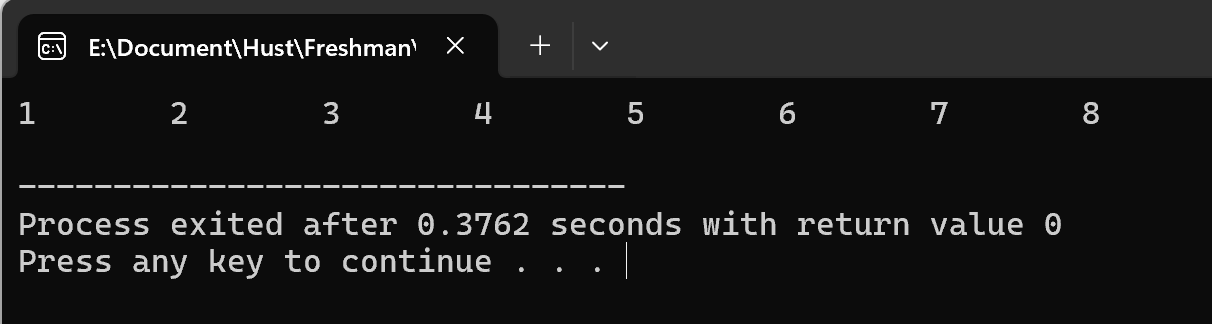
\includegraphics[scale=0.70]{images/7-2-1.png}
					\caption{执行示例}
					\label{pic7-2-1}
				\end{center}
			\end{figure}
			可以见到，通过上述(\ref{pic7-2-1})修正，解决了原程序中参数传递、变量使用、循环判断以及链表头指针传递等方面存在的问题，使得程序能够按照要求，根据给定的整数数组（以 0 作为结束标志）正确构建先进先出的链表，并在 main 函数中成功遍历输出链表中的节点数据。
			
			\subsubsection{7-3 源程序修改替换（二）}
			\subsubsubsection{目标内容}
			(2)	修改替换create\_list 函数,将其建成一个后进先出的链表,后进先出链表的头指针始终指向最后创建的结点(链头),后建结点指向先建结点,先建结点始终是尾结点。
			\subsubsubsection{分析}
			构建后进先出链表与先进先出链表的关键区别在于节点插入的顺序。先进先出链表是新节点依次添加到链表尾部，就像排队一样，先到的排在前面（链表头），后到的排在后面（链表尾）；而后进先出链表则类似栈的操作，新节点要插入到链表头部，后加入的节点成为链表头，这样在后续遍历输出时，后加入的节点会先被访问到，符合后进先出的特性。
			
			\subsubsubsection{相关代码}
			相关代码(\ref{lst:7-3-1})：
			\begin{lstlisting}[style=commonCodeStyle, caption={示例}, label={lst:7-3-1}]
				#include <stdio.h>
				#include <stdlib.h>
				
				struct s_list
				{
					int data;
					struct s_list *next;
				};
				
				void create_list(struct s_list **headp, int *p);
				int main(void)
				{
					struct s_list *head = NULL;
					int s[] = {1, 2, 3, 4, 5, 6, 7, 8, 0};
					create_list(&head, s);
					struct s_list *p = head;
					while (p)
					{
						printf("%d\t", p->data);
						p = p->next;
					}
					printf("\n");
					
					return 0;
				}
				
				void create_list(struct s_list **headp, int *p)
				{
					struct s_list *new_node;
					if (*p == 0)
					{
						return;
					}
					else
					{
						while (*p!= 0)
						{
							new_node = (struct s_list *)malloc(sizeof(struct s_list));
							new_node->data = *p++;
							new_node->next = *headp;
							*headp = new_node;
						}
					}
				}
			\end{lstlisting}
			
			\subsubsubsection{执行结果}
			执行结果(\ref{pic7-3-1})
			\begin{figure}[H]
				\begin{center}
					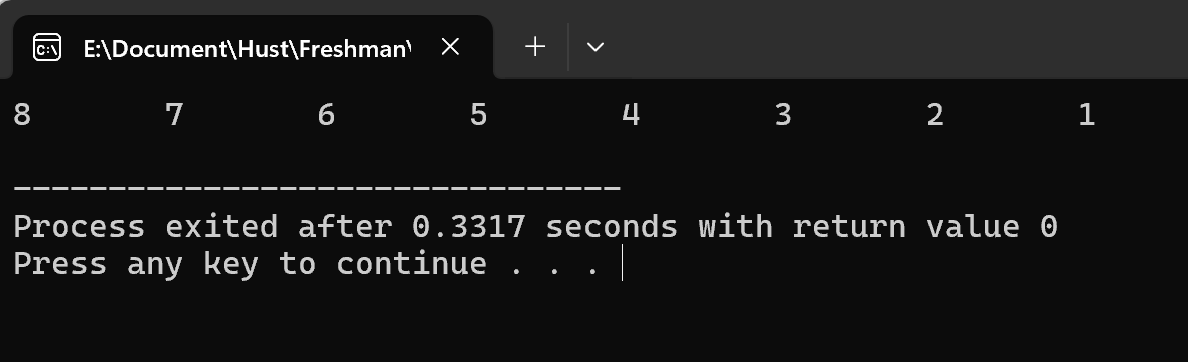
\includegraphics[scale=0.70]{images/7-3-1.png}
					\caption{执行示例}
					\label{pic7-3-1}
				\end{center}
			\end{figure}

		\subsection{程序设计}
			\subsubsection{7-4 设计字段结构}
			\subsubsubsection{目标内容}
			    设计一个字段结构 struct bits, 它将一个 8 位无符号字节从最低位到最高位声明为 8 个字段，依次为 bit0, bit1,..., bit7，且 bit0 优先级最高。同时设计8个函数，第 i 个函数以 biti(i=0, 1, ..., 7)为参数，并且在函数体内输出 biti 的值。将 8 个函数的名字存入一个函数指针数组 p\_fun。如果 bit0 为 1, 调用 p\_fun[0] 指向的函数。如果 struct bits 中有多位为 1，则根据优先级从高到低顺序依次调用函数指针数组 p\_fun 中相应元素指向的函数。
			\subsubsubsection{分析}
			我们需要设计一个 struct bits 结构体，将一个 8 位无符号字节从最低位到最高位声明为 8 个字段，依次为 bit0, bit1, ..., bit7，且 bit0 优先级最高。同时设计 8 个函数，每个函数以 biti 为参数，并输出 biti 的值。将这 8 个函数的名字存入一个函数指针数组 p\_fun，并根据 biti 的值从高到低调用相应的函数。\\
			总流程图(\ref{pic7-4-1})：
			\begin{figure}[H]
				\begin{center}
					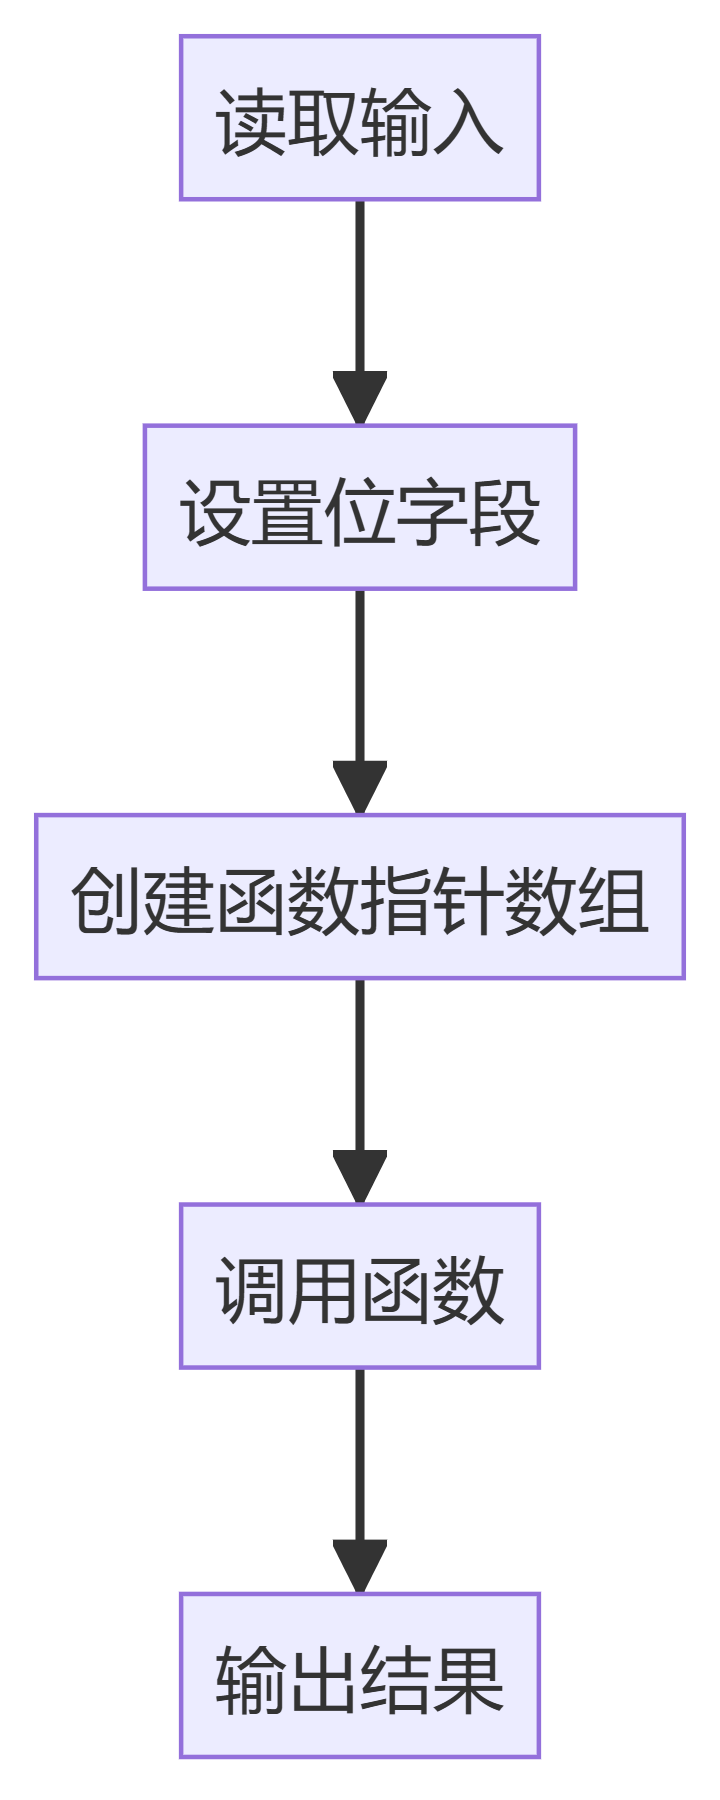
\includegraphics[scale=0.10]{images/7-4-1.png}
					\caption{总流程图}
					\label{pic7-4-1}
				\end{center}
			\end{figure}
			思路：\\
			对于这题主要的可分为两部分：\\
			1.输入处理与位提取：先获取用户输入的整数，然后运用位运算技巧，依次提取该整数二进制表示下每一位的值，并将这些值赋给结构体 struct bits 对应的位域字段，完成数据的初始化准备工作，使得结构体能够准确反映输入整数的二进制位状态。\\
			2.函数调用逻辑构建：创建函数指针数组并初始化其元素为对应的函数地址后，通过循环和条件判断来检查结构体中位域字段的状态。按照从低位到高位（即 bit0 优先级最高，依次到 bit7）的顺序，只要发现某位的值为 1，就调用函数指针数组中对应下标的函数，同时将该位清零，保证每个置位的位对应的函数只会被调用一次，且遵循优先级顺序，直到所有置位的位对应的函数都调用完毕。\\
			相关流程图(\ref{pic7-4-2})：
			\begin{figure}[H]
				\begin{center}
					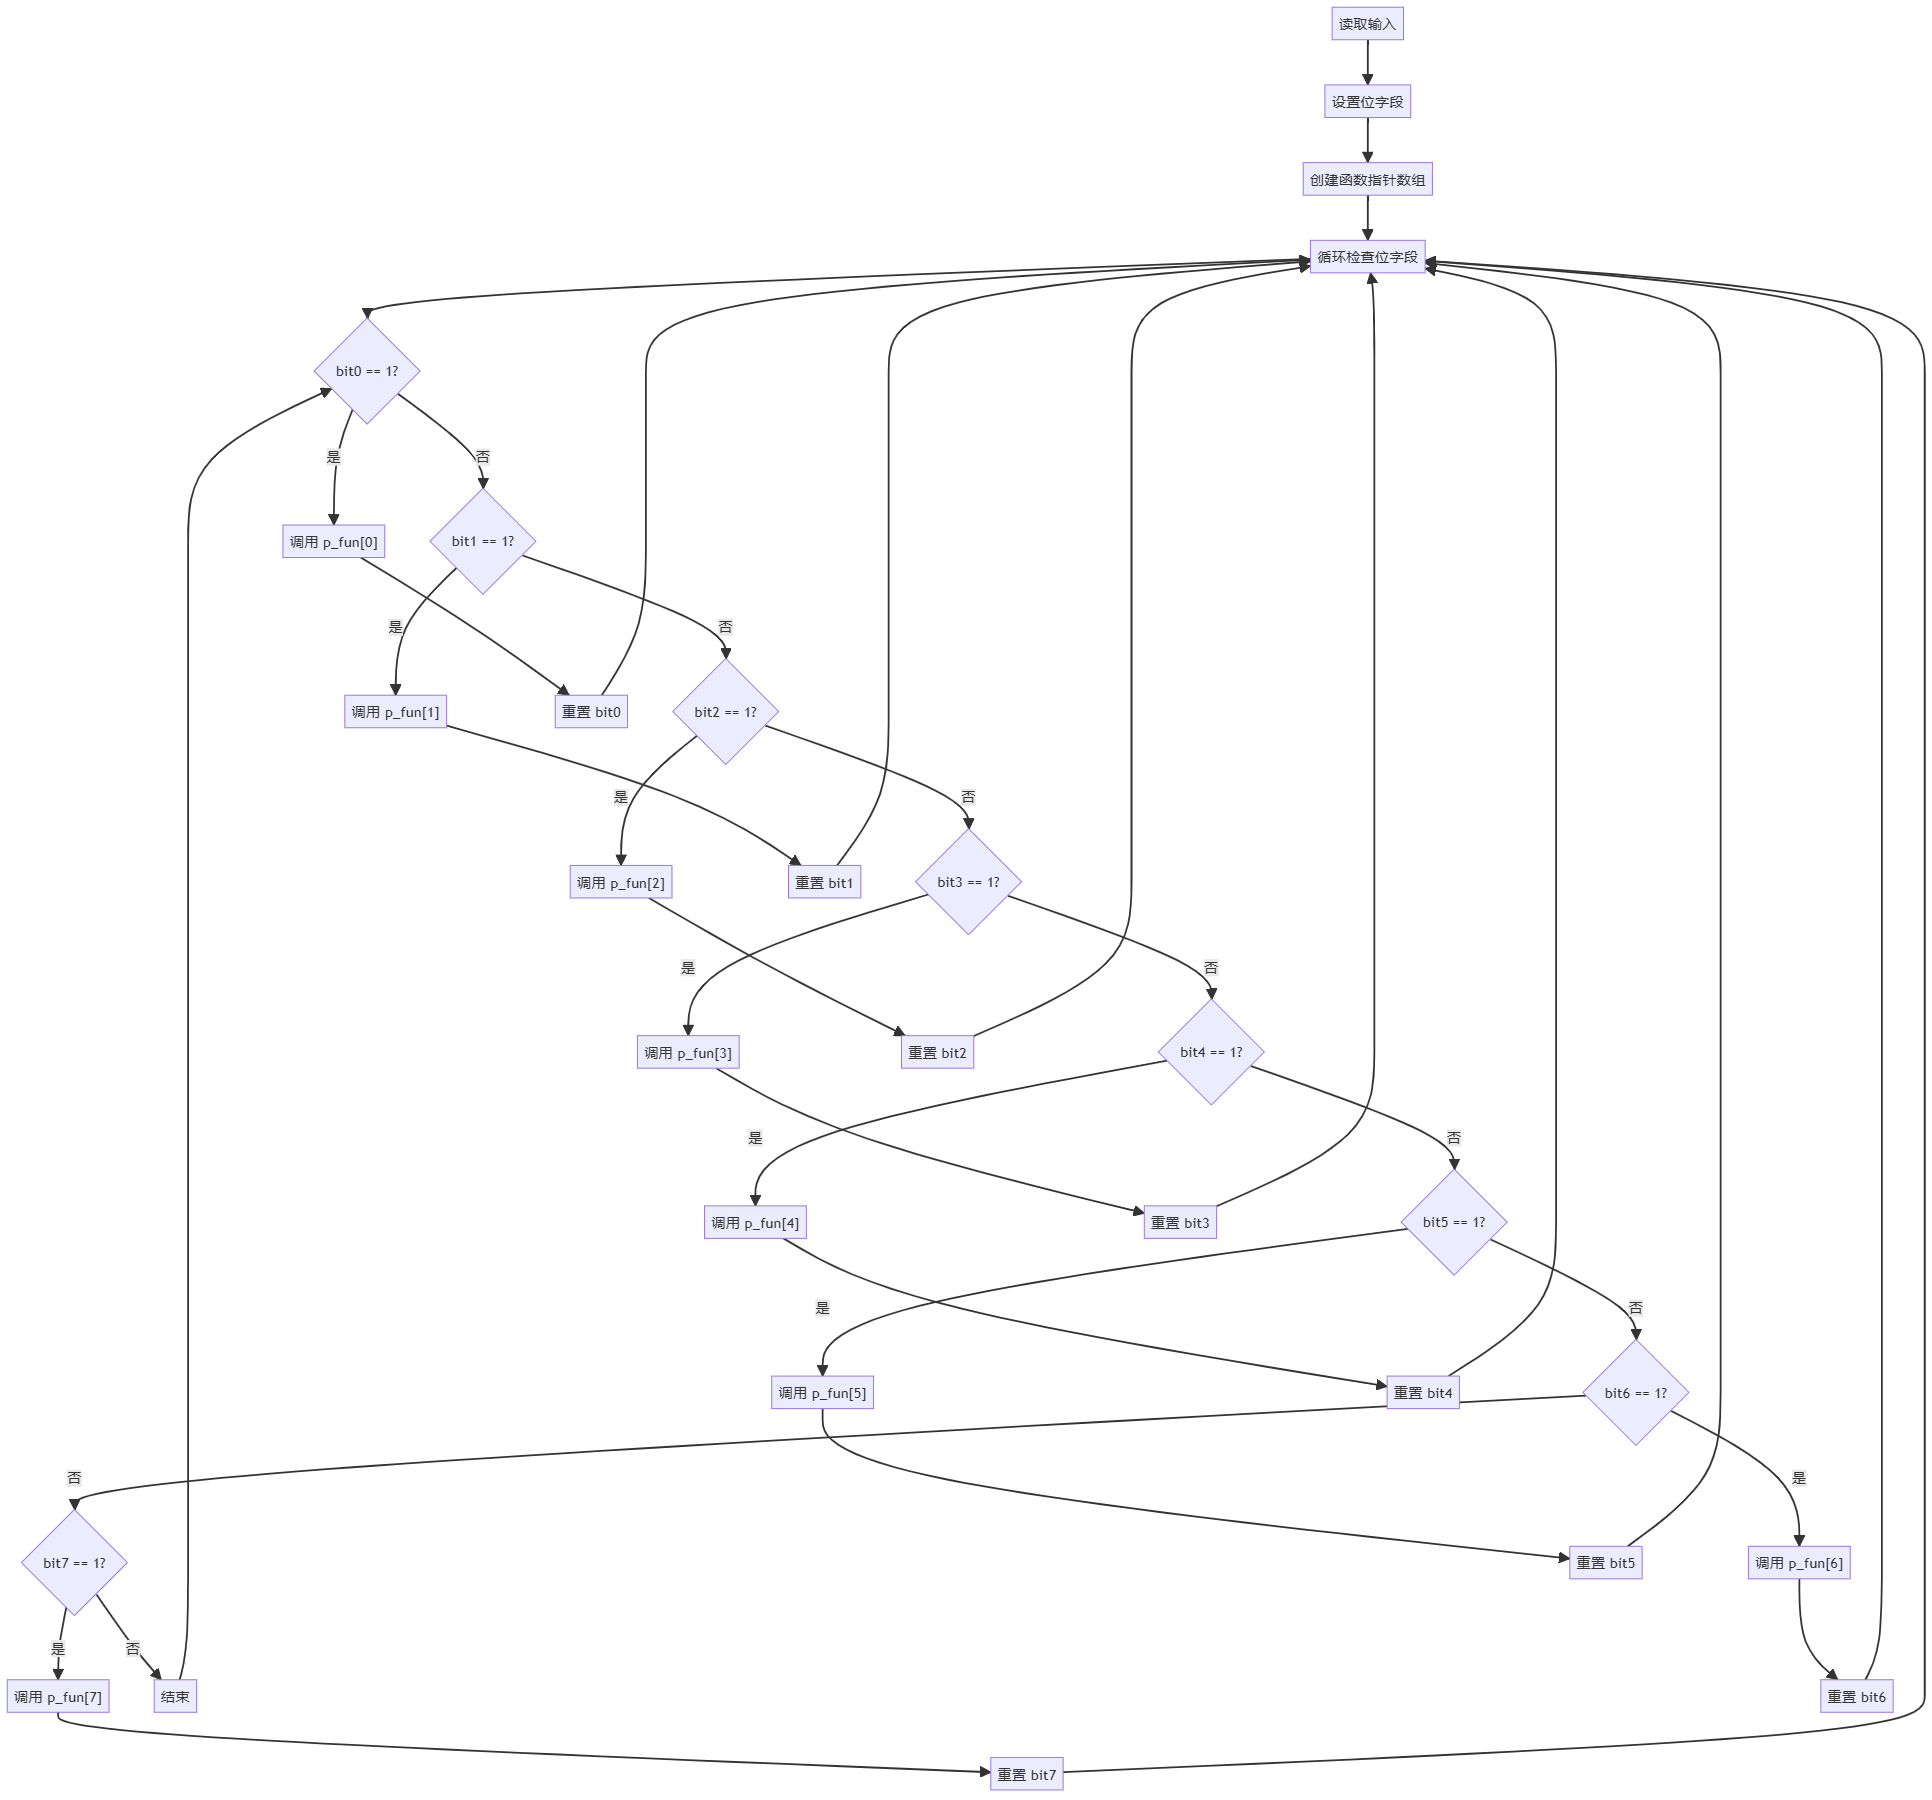
\includegraphics[scale=0.25]{images/7-4-2.png}
					\caption{流程图}
					\label{pic7-4-2}
				\end{center}
			\end{figure}
		
			\subsubsubsection{相关代码}
			相关代码(\ref{lst:7-4-1})：
			
			\begin{lstlisting}[style=commonCodeStyle, caption={示例}, label={lst:7-4-1}]
			#include <stdio.h>
			struct bits {
				unsigned int bit0 : 1;
				unsigned int bit1 : 1;
				unsigned int bit2 : 1;
				unsigned int bit3 : 1;
				unsigned int bit4 : 1;
				unsigned int bit5 : 1;
				unsigned int bit6 : 1;
				unsigned int bit7 : 1;
			};
			void f0(int b) {
				printf("the function %d is called!\n", b);
			}
			
			void f1(int b) {
				printf("the function %d is called!\n", b);
			}
			
			void f2(int b) {
				printf("the function %d is called!\n", b);
			}
			
			void f3(int b) {
				printf("the function %d is called!\n", b);
			}
			
			void f4(int b) {
				printf("the function %d is called!\n", b);
			}
			
			void f5(int b) {
				printf("the function %d is called!\n", b);
			}
			
			void f6(int b) {
				printf("the function %d is called!\n", b);
			}
			
			void f7(int b) {
				printf("the function %d is called!\n", b);
			}
			int main() {
				struct bits byte;
				int num;
				scanf("%d", &num);
				byte.bit0 = num & 1;
				byte.bit1 = (num >> 1) & 1;
				byte.bit2 = (num >> 2) & 1;
				byte.bit3 = (num >> 3) & 1;
				byte.bit4 = (num >> 4) & 1;
				byte.bit5 = (num >> 5) & 1;
				byte.bit6 = (num >> 6) & 1;
				byte.bit7 = (num >> 7) & 1;
				void (*p_fun[8])(int) = {f0, f1, f2, f3, f4, f5, f6, f7};
				for (int i = 0; i < 8; i++) {
					if (byte.bit0 + byte.bit1 + byte.bit2 + byte.bit3 + byte.bit4 + byte.bit5 + byte.bit6 + byte.bit7 > 0) {
						int index = 0;
						while (byte.bit0 + byte.bit1 + byte.bit2 + byte.bit3 + byte.bit4 + byte.bit5 + byte.bit6 + byte.bit7 > 0) {
							if (byte.bit0 == 1) {
								p_fun[0](0);
								byte.bit0 = 0;
							}
							else if (byte.bit1 == 1) {
								p_fun[1](1);
								byte.bit1 = 0;
							}
							else if (byte.bit2 == 1) {
								p_fun[2](2);
								byte.bit2 = 0;
							}
							else if (byte.bit3 == 1) {
								p_fun[3](3);
								byte.bit3 = 0;
							}
							else if (byte.bit4 == 1) {
								p_fun[4](4);
								byte.bit4 = 0;
							}
							else if (byte.bit5 == 1) {
								p_fun[5](5);
								byte.bit5 = 0;
							}
							else if (byte.bit6 == 1) {
								p_fun[6](6);
								byte.bit6 = 0;
							}
							else if (byte.bit7 == 1) {
								p_fun[7](7);
								byte.bit7 = 0;
							}
						}
						break;
					}
				}
				return 0;
			}
			\end{lstlisting}
			
			
			\subsubsubsection{执行结果}
			执行结果(\ref{pic7-4-3}\ref{pic7-4-4})
			\begin{figure}[H]
				\begin{center}
					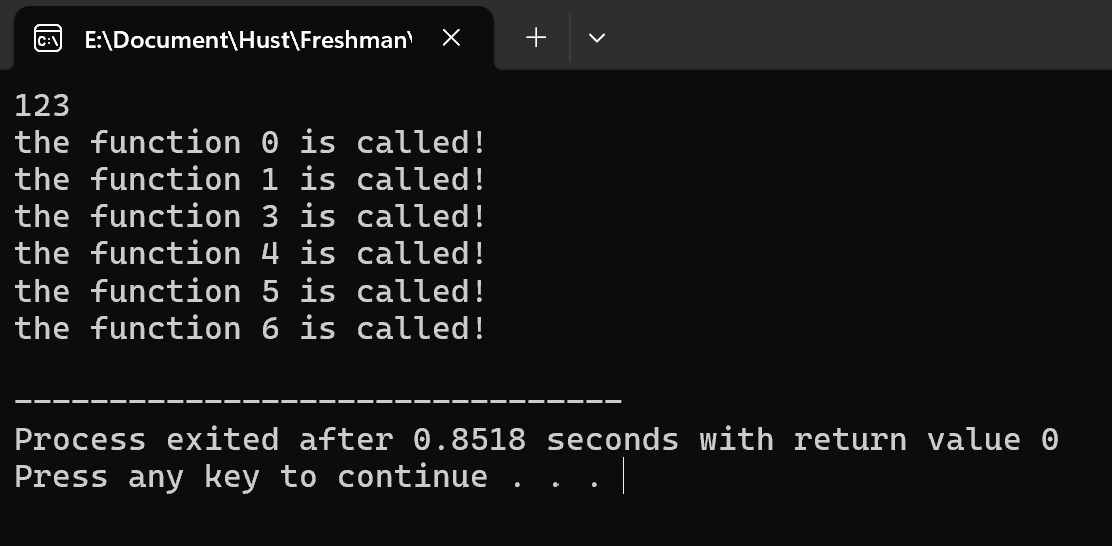
\includegraphics[scale=0.70]{images/7-4-3.png}
					\caption{执行示例}
					\label{pic7-4-3}
				\end{center}
			\end{figure}
			\begin{figure}[H]
			\begin{center}
				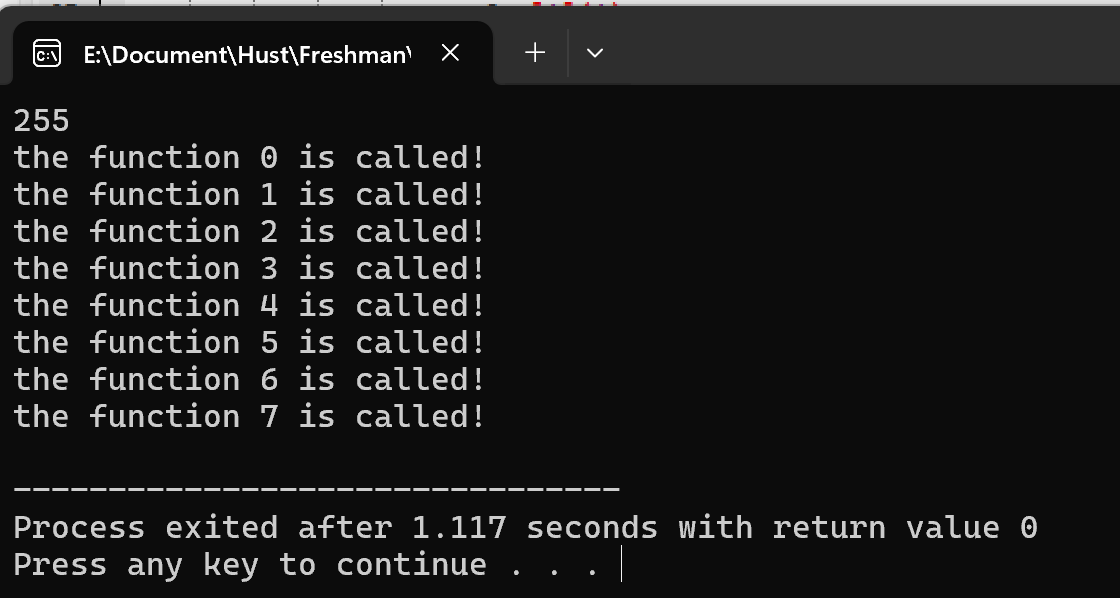
\includegraphics[scale=0.70]{images/7-4-4.png}
				\caption{执行示例}
				\label{pic7-4-4}
			\end{center}
			\end{figure}
			可见，通过前面的分析，设计，程序能够正确地解析输入的 8 位无符号整数，并根据位字段的值从高到低调用相应的函数。
			
\newpage
			\subsubsection{7-5 班级成绩单}
			\subsubsubsection{目标内容}
			用单向链表建立一张班级成绩单，包括每个学生的学号、姓名、英语、高等数学、普通物理、C语言程序设计4门课程的成绩。实现以下功能，并提供菜单选项：\\
			0.退出\\
			1.输入每个学生的各项信息\\
			2.输出每个学生的各项信息\\
			3.修改指定学生的指定数据项的内容：\\
			1.修改英语成绩\\
			2.修改高等数学成绩\\
			3.修改普通物理成绩\\
			4.修改C语言成绩\\
			4.统计每个学生的平均成绩（保留2位小数）\\
			5.输出各位学生的学号、姓名、4门课程的总成绩和平均成绩\\
			\subsubsubsection{分析}
			这题的目标内容和数组的实验题几许相似，我们需要利用结构体和模块化的设计思路去进行分块设计。有助于我们去一步步完成这题的设计。\\
			总流程图(\ref{pic7-5-1})：
			\begin{figure}[H]
				\begin{center}
					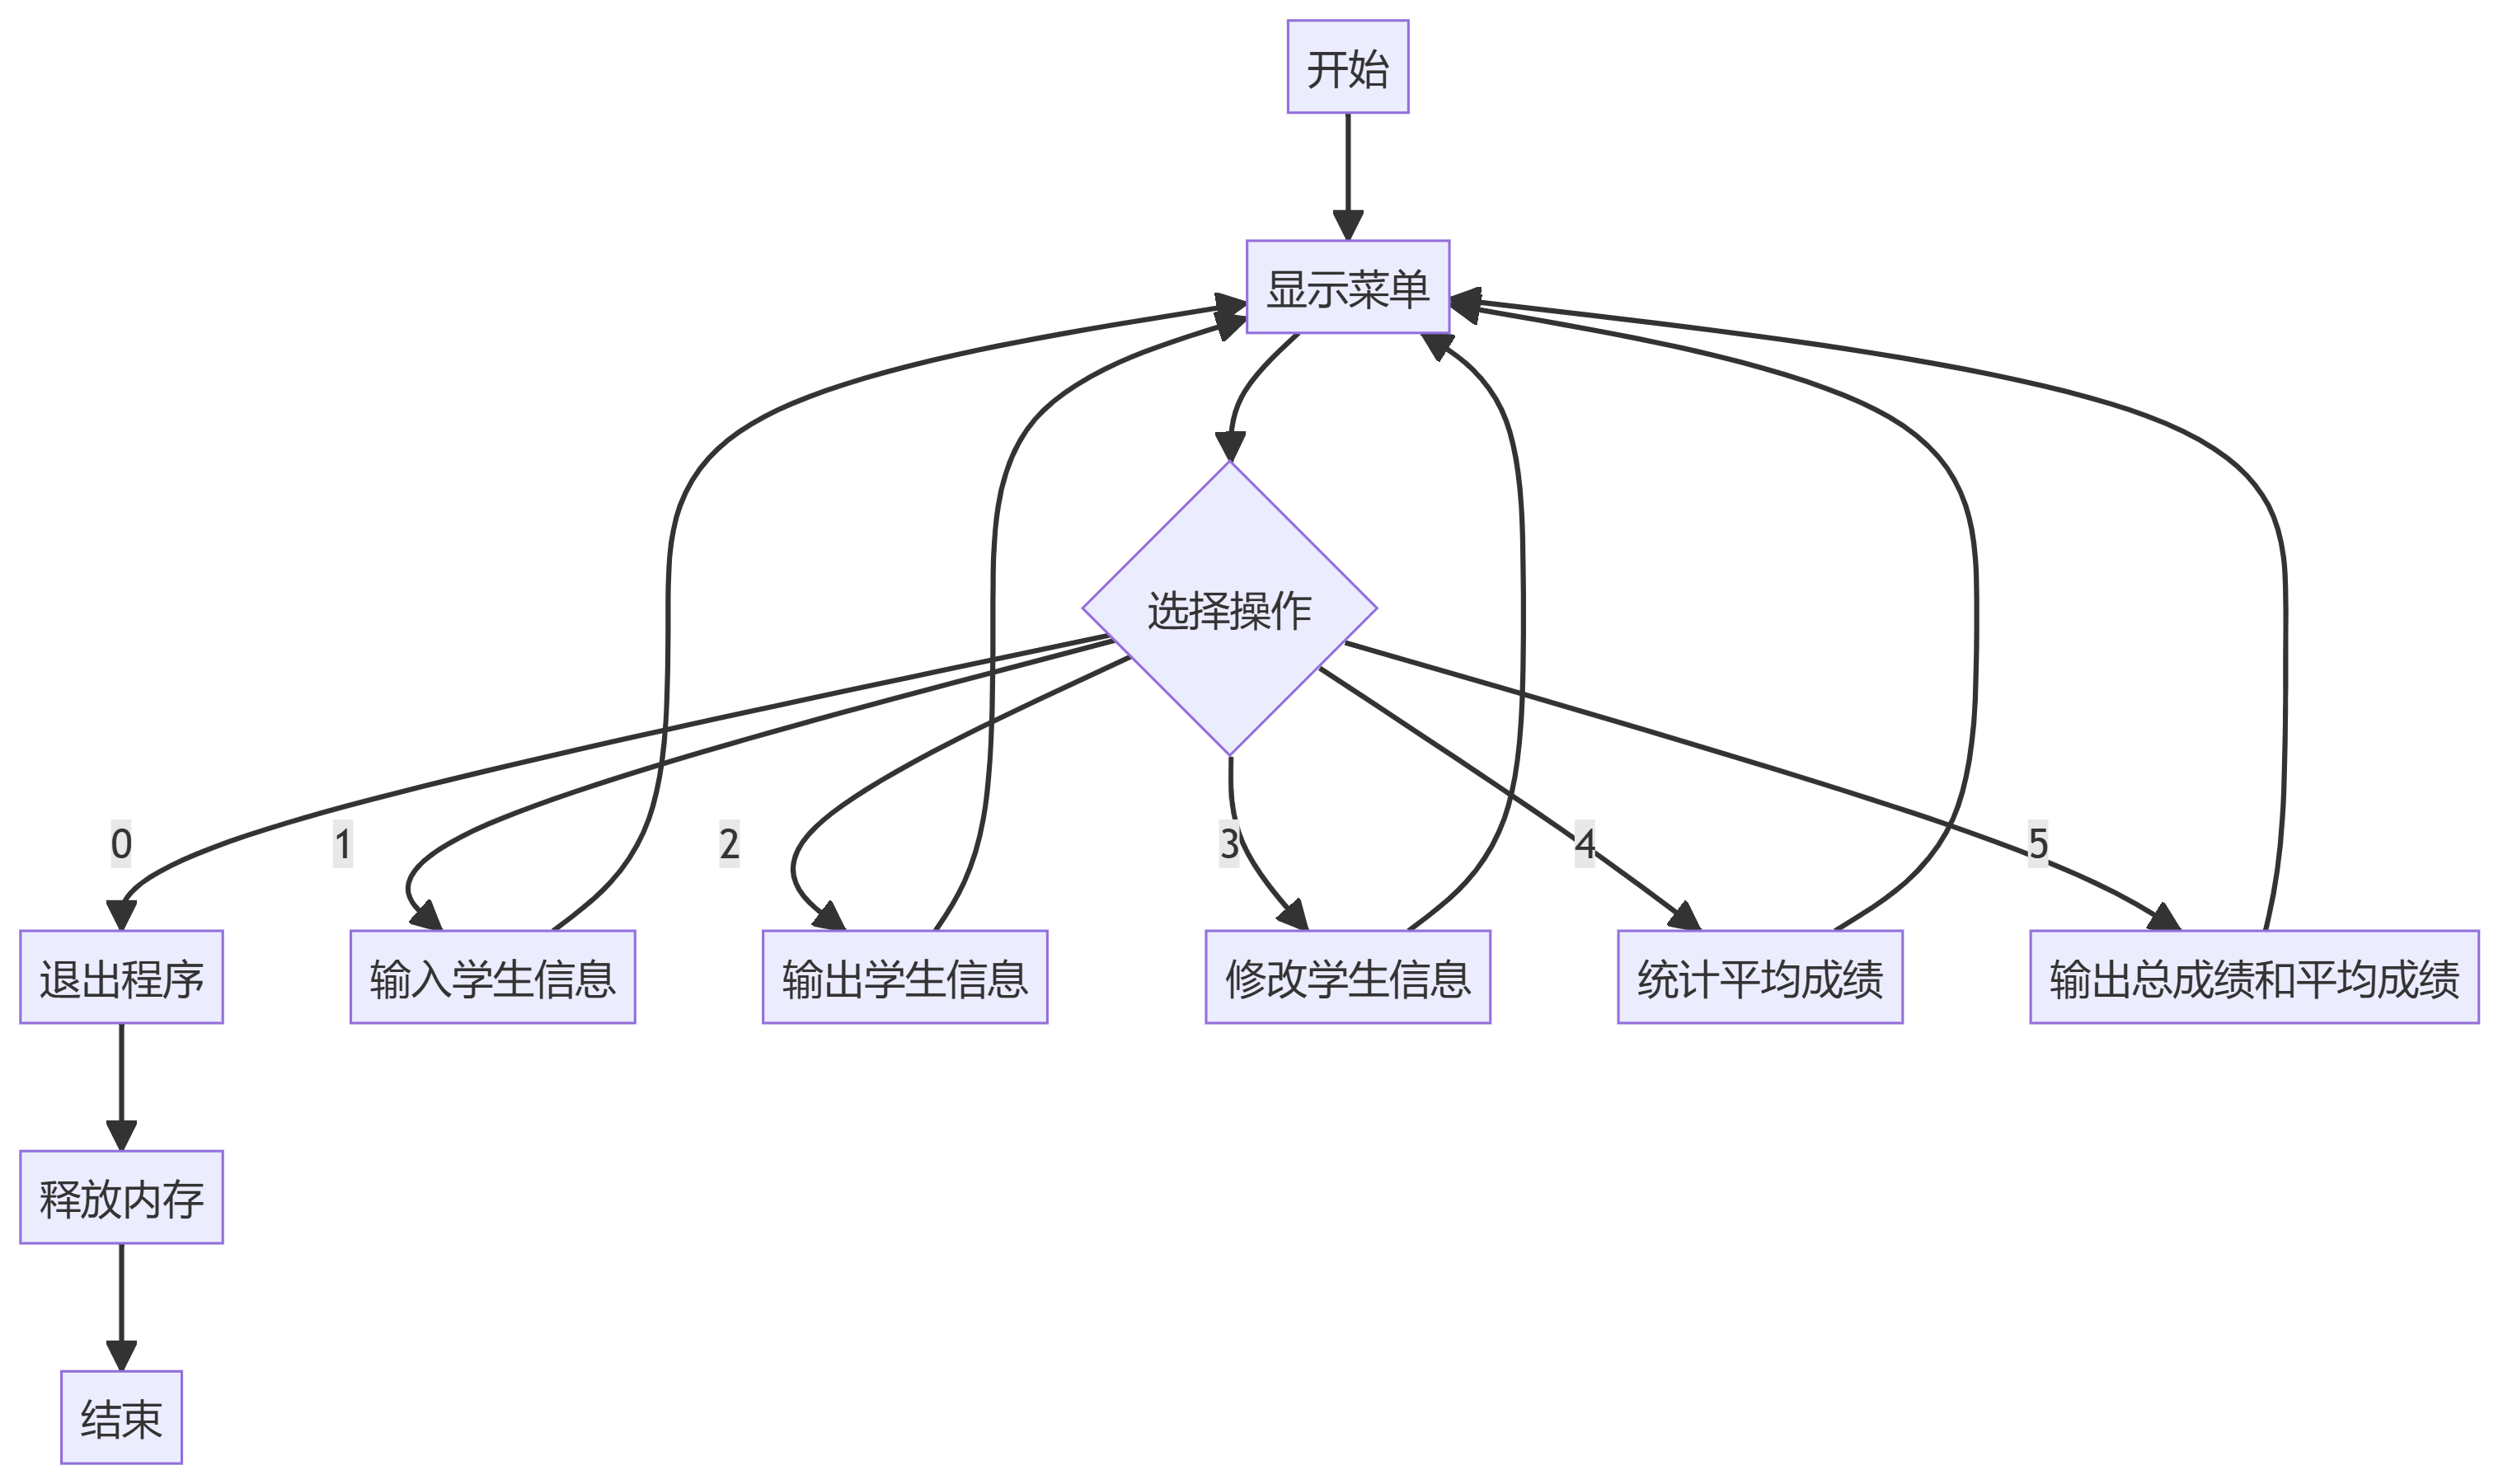
\includegraphics[scale=0.12]{images/7-5-1.png}
					\caption{总流程图}
					\label{pic7-5-1}
				\end{center}
			\end{figure}
			設計思路：\\
			选用单向链表来存储班级学生的成绩单信息，是因为班级学生数量不确定，链表这种动态数据结构可以方便地根据需要添加或删除节点，灵活地管理不同数量的学生数据。每个链表节点对应一个学生，节点结构体中包含了存储学生各项信息（学号、姓名、四门课程成绩以及平均成绩）的成员变量，以及一个指向下一个节点的指针，通过指针将各个节点串联起来形成完整的成绩单链表。
			通过 构建函数创建单个学生节点并初始化各项成员变量（含成绩赋值与平均成绩计算），构建新函数将新节点添加到链表中，处理链表为空和不为空的添加逻辑，以此构建整个班级成绩单链表；再设计函数按不同需求输出学生详细信息、用自定义的函数输出平均成绩、函数输出学号、姓名、总成绩及平均成绩等多个输出函数，它们都通过遍历链表展示相应信息方便用户查看不同格式成绩单内容；再设计函数可遍历链表查找匹配学号的节点，依据用户所选课程选项更新成绩并重新算平均成绩来实现修改指定学生指定课程成绩功能，保证数据准确一致；在 main 函数里利用无限循环和 switch 语句构建菜单驱动的程序框架，按用户输入选项调用相应功能函数实现交互及各功能调度，且退出程序选项中考虑释放链表内存资源以避免内存泄漏问题。
			相关流程图(\ref{pic7-5-2})：
			\begin{figure}[H]
				\begin{center}
					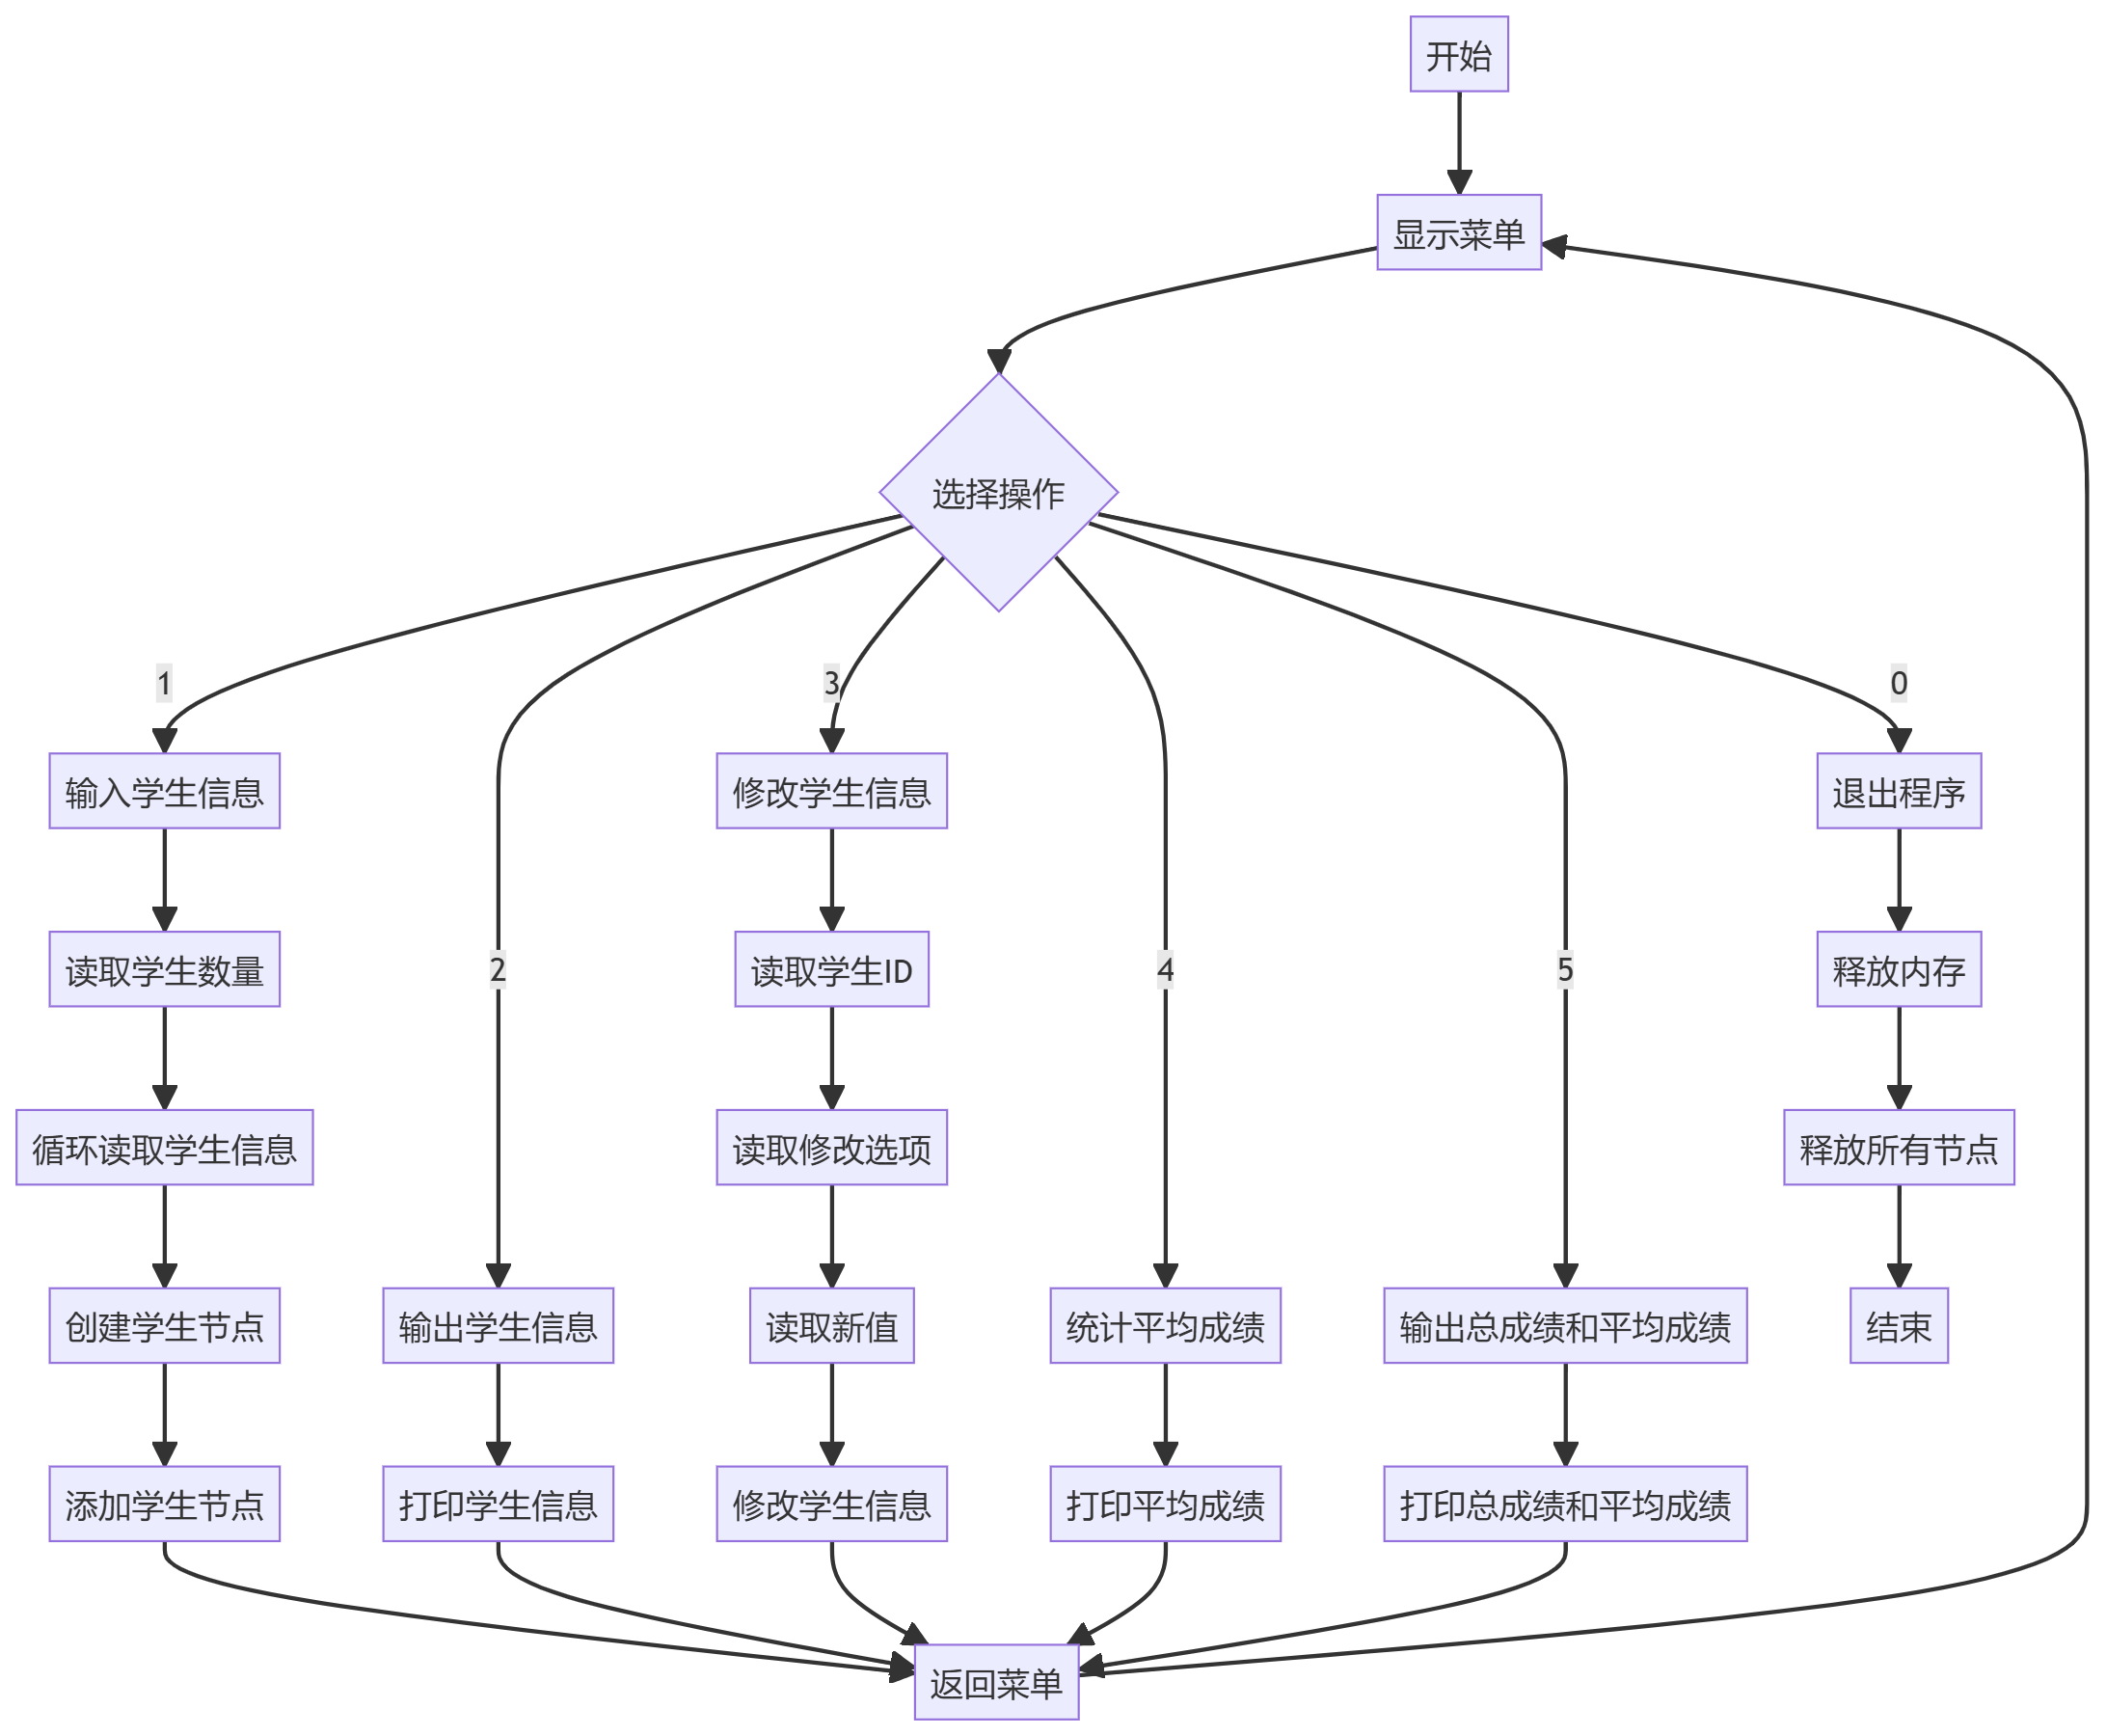
\includegraphics[scale=0.20]{images/7-5-2.png}
					\caption{流程图}
					\label{pic7-5-2}
				\end{center}
			\end{figure}
			
			\subsubsubsection{相关代码}
			相关代码(\ref{lst:7-5-1})：
			\begin{lstlisting}[style=commonCodeStyle, caption={示例}, label={lst:7-5-1}]
				#include <stdio.h>
				#include <stdlib.h>
				#include <string.h>
				#include <math.h>
				#define NAME_LEN 50
				typedef struct Student {
					char id[20];
					char name[NAME_LEN];
					float english;
					float math;
					float physics;
					float c_programming;
					float average;
					struct Student* next;
				} Student;
				Student* createNode(char* id, char* name, float english, float math, float physics, float c_programming) {
					Student* newNode = (Student*)malloc(sizeof(Student));
					if (newNode == NULL) {
						exit(1);
					}
					strcpy(newNode->id, id);
					strcpy(newNode->name, name);
					newNode->english = english;
					newNode->math = math;
					newNode->physics = physics;
					newNode->c_programming = c_programming;
					newNode->average = (english + math + physics + c_programming) / 4.0;
					newNode->next = NULL;
					return newNode;
				}
				void addStudent(Student** head, char* id, char* name, float english, float math, float physics, float c_programming) {
					Student* newNode = createNode(id, name, english, math, physics, c_programming);
					if (*head == NULL) {
						*head = newNode;
					} else {
						Student* temp = *head;
						while (temp->next != NULL) {
							temp = temp->next;
						}
						temp->next = newNode;
					}
				}
				void printStudents(Student* head, int isAveragePrinted) {
					Student* temp = head;
					while (temp != NULL) {
						printf("%s %s ", temp->id, temp->name);
						if (isAveragePrinted) {
							printf("%.2f ", temp->english);
							printf("%.2f ", temp->math);
							printf("%.2f ", temp->physics);
							printf("%.2f\n", temp->c_programming);
						} else {
							if (floor(temp->english) == temp->english) {
								printf("%d ", (int)temp->english);
							} else {
								printf("%.2f ", temp->english);
							}
							if (floor(temp->math) == temp->math) {
								printf("%d ", (int)temp->math);
							} else {
								printf("%.2f ", temp->math);
							}
							if (floor(temp->physics) == temp->physics) {
								printf("%d ", (int)temp->physics);
							} else {
								printf("%.2f ", temp->physics);
							}
							if (floor(temp->c_programming) == temp->c_programming) {
								printf("%d\n", (int)temp->c_programming);
							} else {
								printf("%.2f\n", temp->c_programming);
							}
						}
						temp = temp->next;
					}
				}
				void modifyStudent(Student* head, char* id, int choice, float newValue) {
					Student* temp = head;
					while (temp != NULL) {
						if (strcmp(temp->id, id) == 0) {
							switch (choice) {
								case 1:
								temp->english = newValue;
								break;
								case 2:
								temp->math = newValue;
								break;
								case 3:
								temp->physics = newValue;
								break;
								case 4:
								temp->c_programming = newValue;
								break;
							}
							temp->average = (temp->english + temp->math + temp->physics + temp->c_programming) / 4.0;
							return;
						}
						temp = temp->next;
					}
				}
				void printAverages(Student* head) {
					Student* temp = head;
					while (temp != NULL) {
						printf("%s %s ", temp->id, temp->name);
						printf("%.2f\n", temp->average);
						temp = temp->next;
					}
				}
				void printTotalAndAverage(Student* head) {
					Student* temp = head;
					while (temp != NULL) {
						float total = temp->english + temp->math + temp->physics + temp->c_programming;
						printf("%s %s %d %.2f\n", temp->id, temp->name, (int)total, temp->average);
						temp = temp->next;
					}
				}
				int main() {
					Student* head = NULL;
					int choice, n;
					char id[20], name[NAME_LEN];
					float english, math, physics, c_programming;
					char modifyId[20];
					int modifyChoice;
					float newValue;
					int isAveragePrinted = 0;
					while (1) {
						scanf("%d", &choice);
						
						switch (choice) {
							case 0:
							while (head != NULL) {
								Student* temp = head;
								head = head->next;
								free(temp);
							}
							exit(0);
							case 1:
							scanf("%d", &n);
							for (int i = 0; i < n; i++) {
								scanf("%s %s %f %f %f %f", id, name, &english, &math, &physics, &c_programming);
								addStudent(&head, id, name, english, math, physics, c_programming);
							}
							break;
							case 2:
							printStudents(head, isAveragePrinted);
							break;
							case 3:
							scanf("%s %d %f", modifyId, &modifyChoice, &newValue);
							modifyStudent(head, modifyId, modifyChoice, newValue);
							break;
							case 4:
							printAverages(head);
							isAveragePrinted = 1;
							break;
							case 5:
							printTotalAndAverage(head);
							break;
						}
					}
					return 0;
				}
			\end{lstlisting}
			\subsubsubsection{执行结果}
			执行结果(\ref{pic7-5-3}\ref{pic7-5-4})：
			\begin{figure}[H]
				\begin{center}
					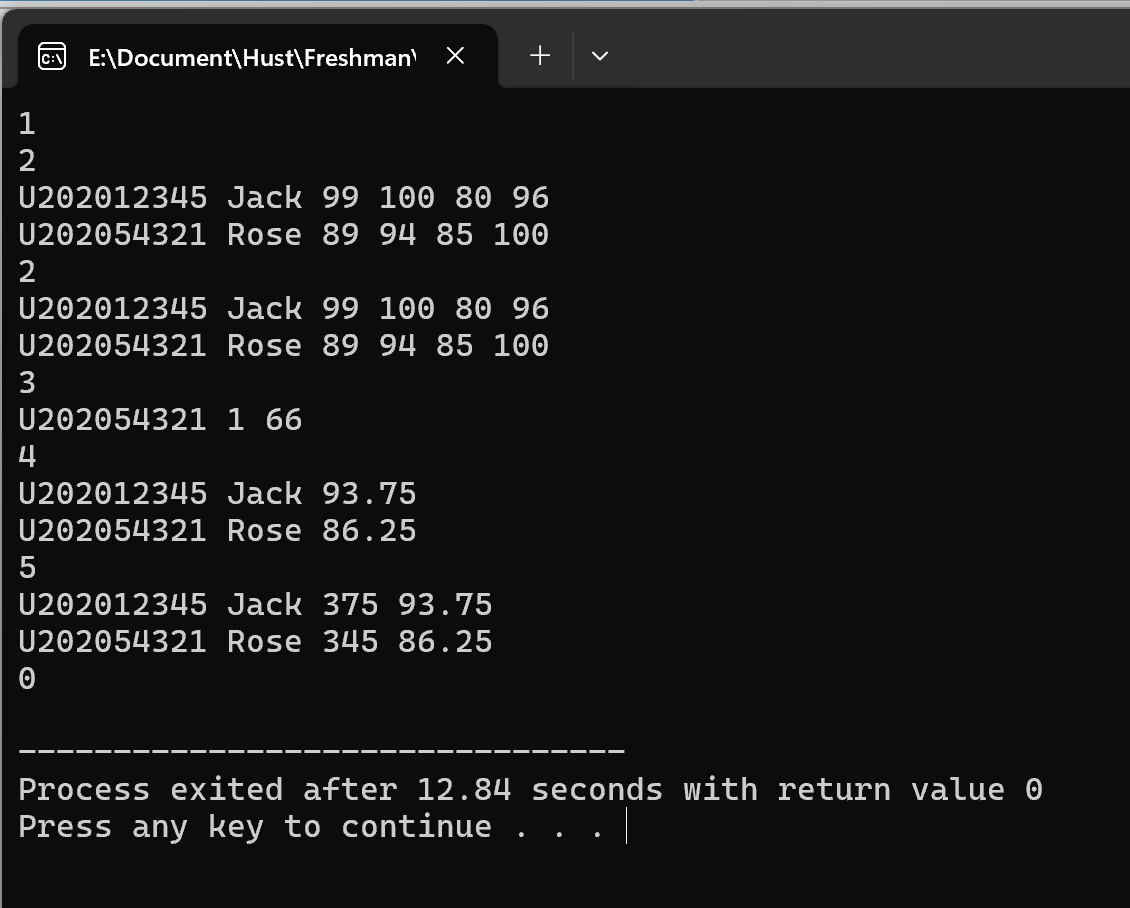
\includegraphics[scale=0.50]{images/7-5-3.png}
					\caption{执行示例}
					\label{pic7-5-3}
				\end{center}
			\end{figure}
		\begin{figure}[H]
			\begin{center}
				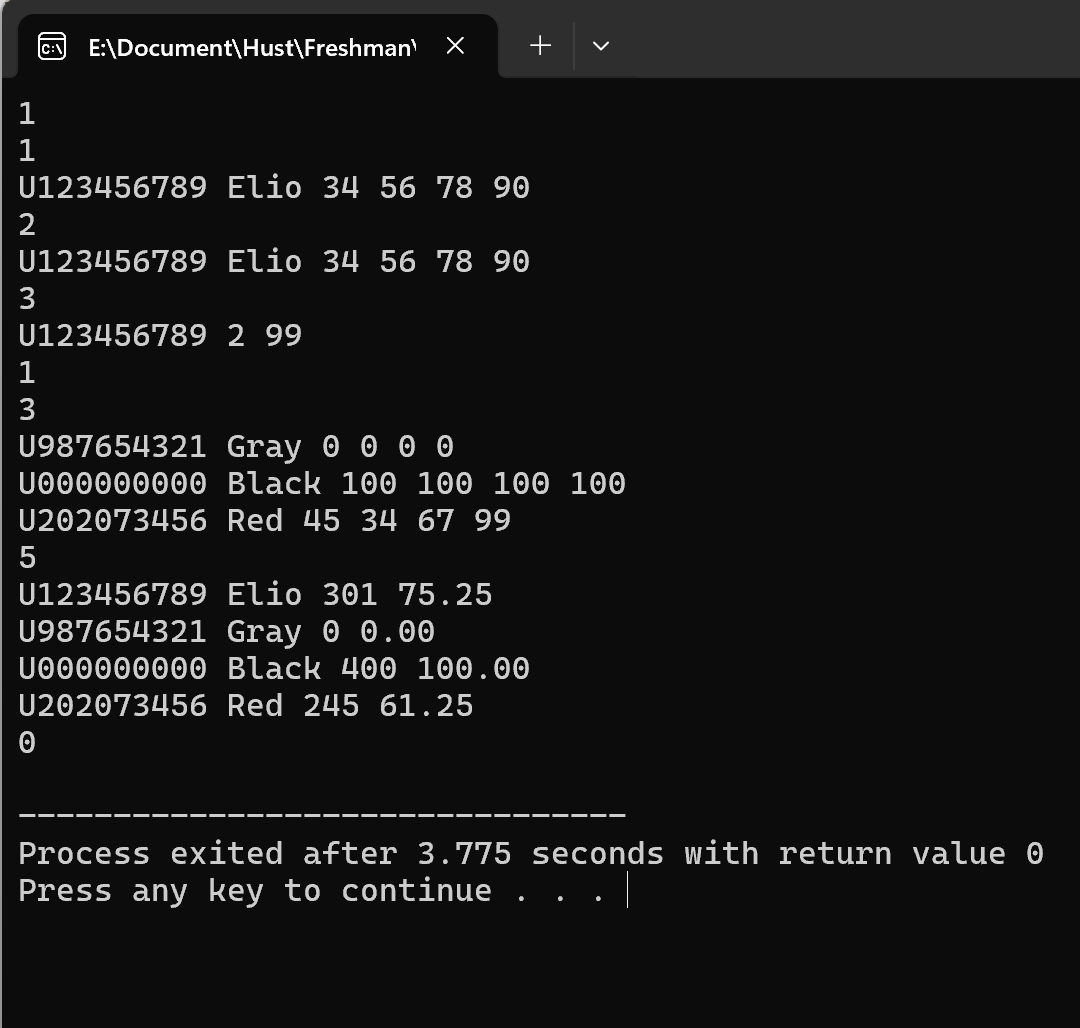
\includegraphics[scale=0.50]{images/7-5-4.png}
				\caption{执行示例}
				\label{pic7-5-4}
			\end{center}
		\end{figure}
		通过输入和处理学生的数据，能够见到本代码在最后是能够顺利输出的，实现了本题的要求，下面把与这题有相关的7-6和7-8题目也一并说明。

\newpage
			\subsubsection{7-6 成绩排序（一）}
			\subsubsubsection{目标内容}
			对程序设计的第二题增加按照平均成绩进行升序排序的函数，写出用交换结点数据域的方法升序排序的函数，排序可用选择法或冒泡法。	
			\subsubsubsection{分析}
			在7-5原有的基础上加入排序的算法，基本上大致的流程结构不用改变多少，主要是在模块化的地方加入新的排序算法，则能使本题成立。
			总流程图(\ref{pic7-5-1})：
			\begin{figure}[H]
				\begin{center}
					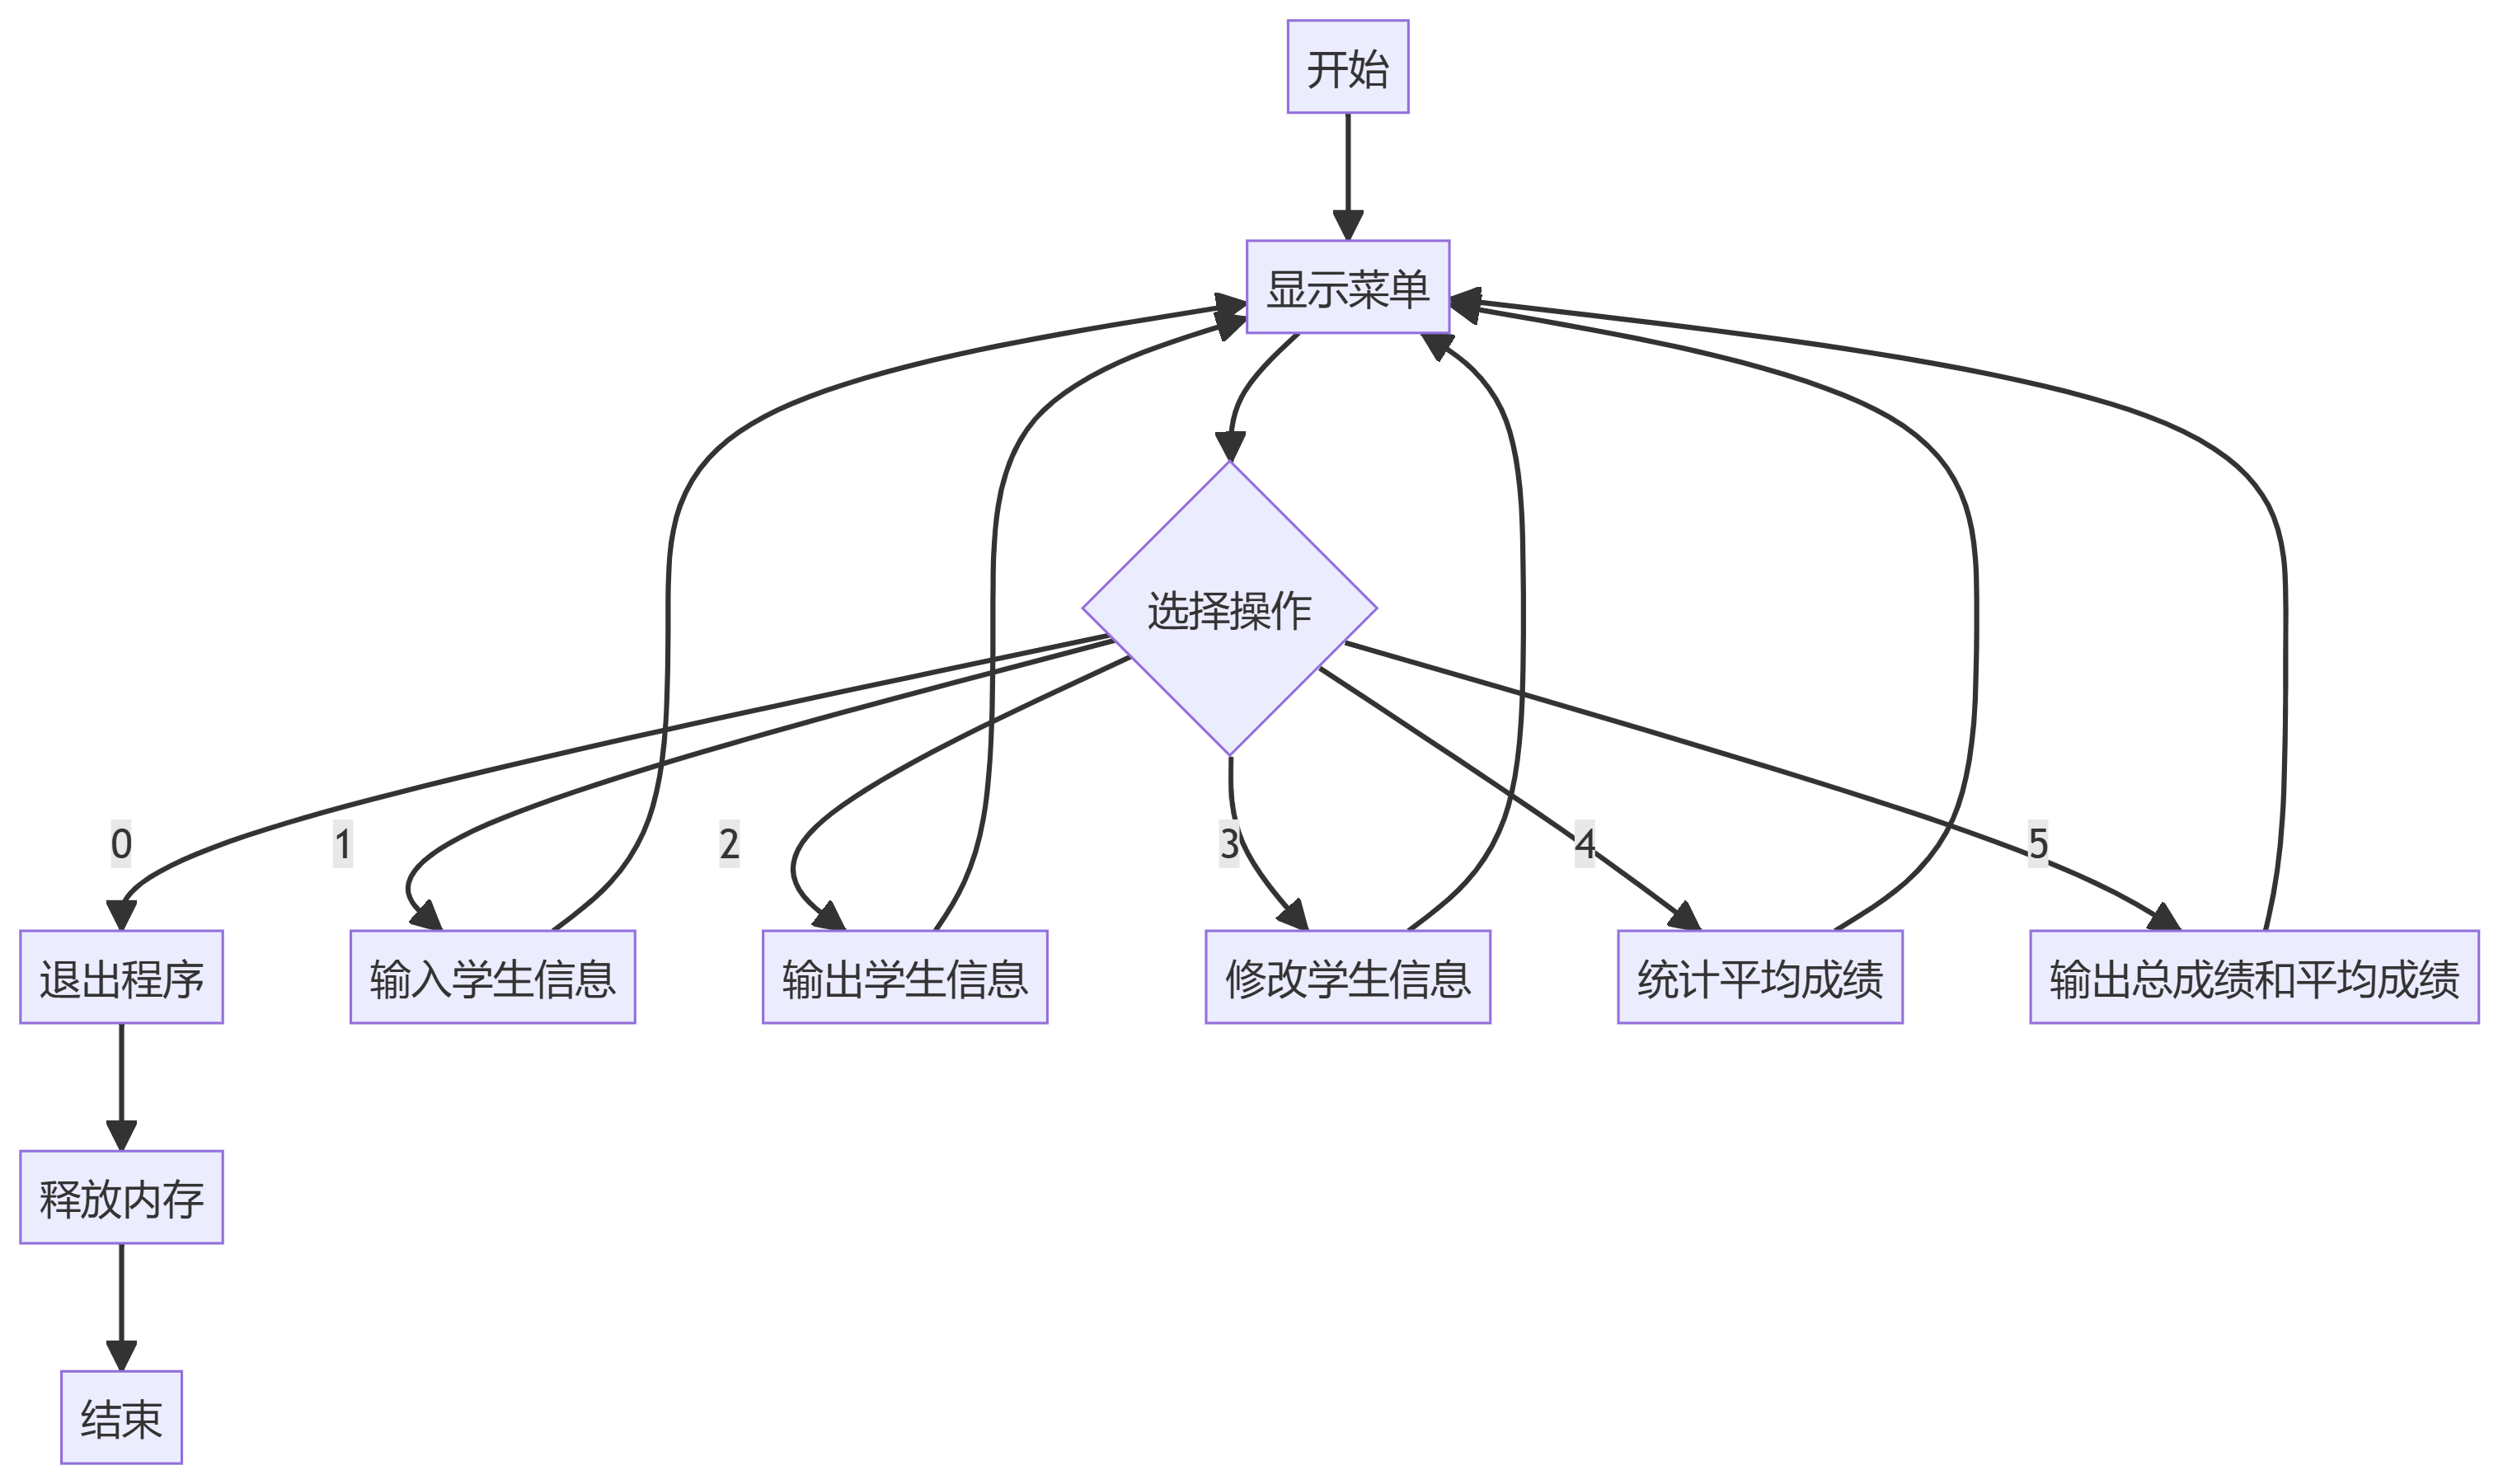
\includegraphics[scale=0.13]{images/7-5-1.png}
					\caption{总流程图}
					\label{pic7-5-1}
				\end{center}
			\end{figure}
			\begin{figure}[H]
			\begin{center}
				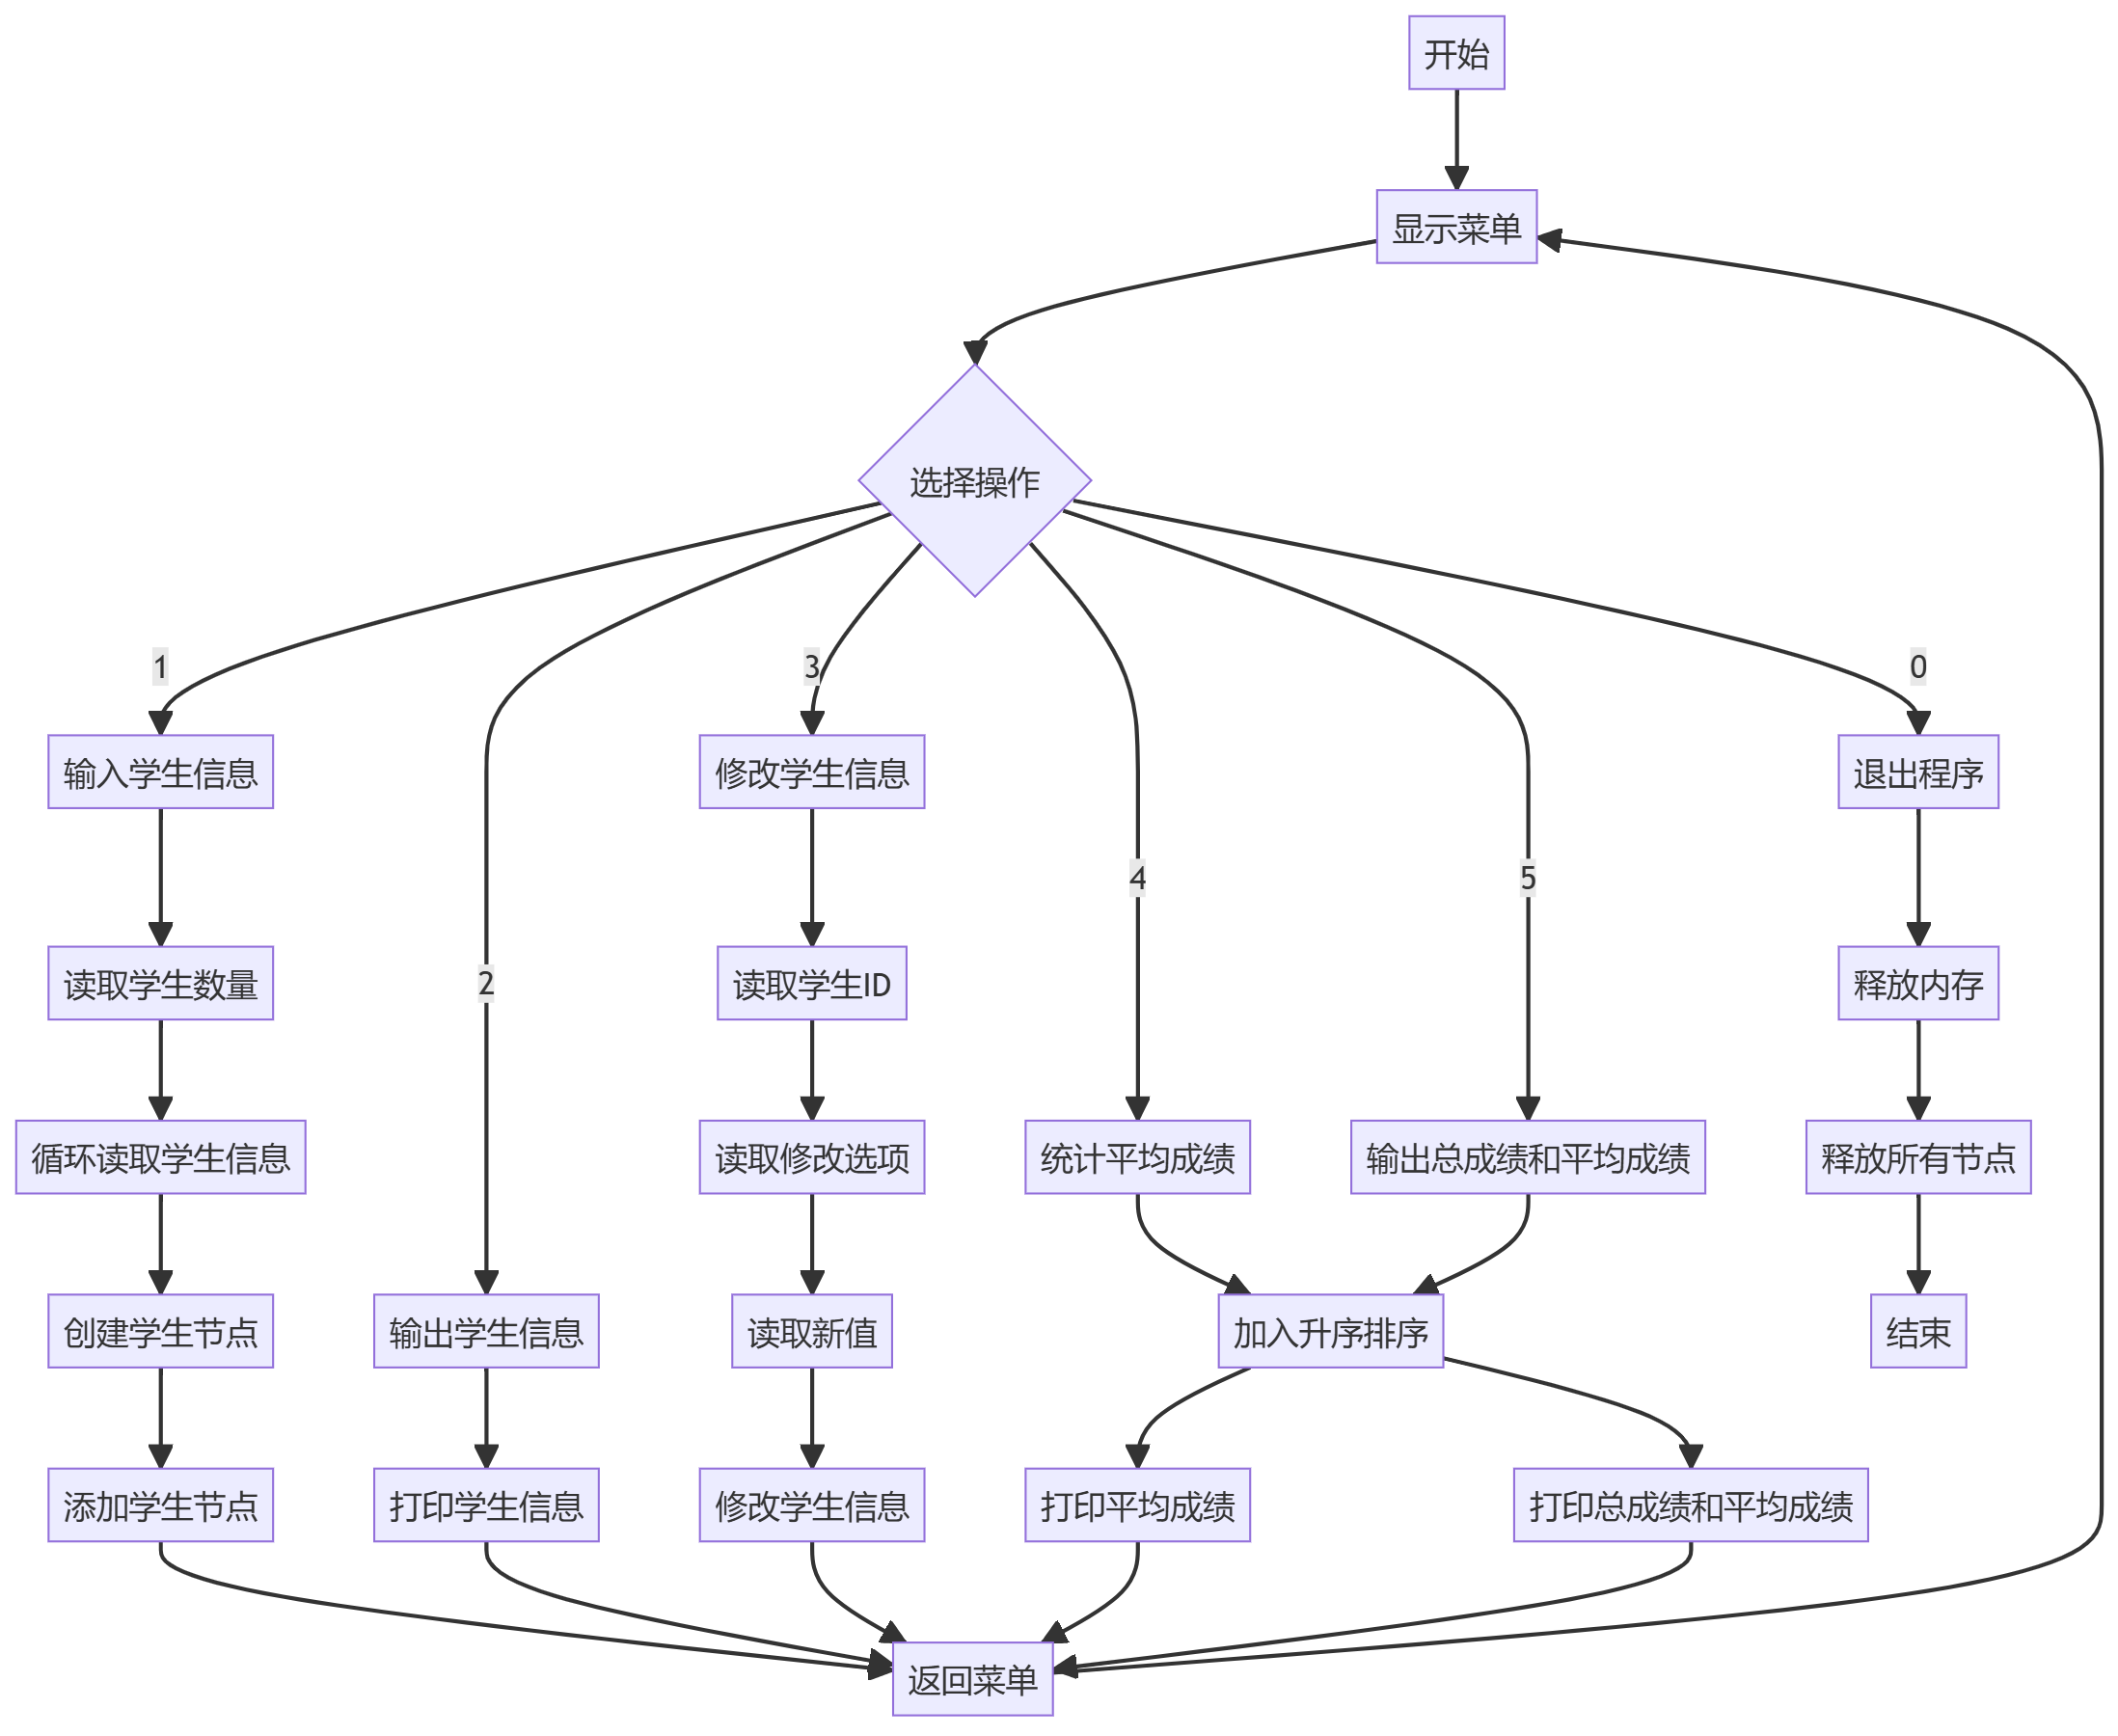
\includegraphics[scale=0.17]{images/7-6-1.png}
				\caption{流程图}
				\label{pic7-6-1}
			\end{center}
			\end{figure}
			
			\subsubsubsection{相关代码}
			相关代码(\ref{lst:7-6-1})：
			\begin{lstlisting}[style=commonCodeStyle, caption={示例}, label={lst:7-6-1}]
				#include <stdio.h>
				#include <stdlib.h>
				#include <string.h>
				#include <math.h>
				#define NAME_LEN 50
				typedef struct Student {
					char id[20];
					char name[NAME_LEN];
					float english;
					float math;
					float physics;
					float c_programming;
					float average;
					struct Student *next;
				} Student;
				Student *createNode(char *id, char *name, float english, float math, float physics, float c_programming);
				void addStudent(Student **head, char *id, char *name, float english, float math, float physics, float c_programming);
				void printStudents(Student *head, int isAveragePrinted);
				void modifyStudent(Student *head, char *id, int choice, float newValue);
				void sortStudentsByAverage(Student **head);
				void printAverages(Student *head);
				void printTotalAndAverage(Student *head);
				Student *createNode(char *id, char *name, float english, float math, float physics, float c_programming) {
					Student *newNode = (Student *)malloc(sizeof(Student));
					if (newNode == NULL) {
						exit(1);
					}
					strcpy(newNode->id, id);
					strcpy(newNode->name, name);
					newNode->english = english;
					newNode->math = math;
					newNode->physics = physics;
					newNode->c_programming = c_programming;
					newNode->average = (english + math + physics + c_programming) / 4.0;
					newNode->next = NULL;
					return newNode;
				}
				void addStudent(Student **head, char *id, char *name, float english, float math, float physics, float c_programming) {
					Student *newNode = createNode(id, name, english, math, physics, c_programming);
					if (*head == NULL) {
						*head = newNode;
					}
					else {
						Student *temp = *head;
						while (temp->next!= NULL) {
							temp = temp->next;
						}
						temp->next = newNode;
					}
				}
				void printStudents(Student *head, int isAveragePrinted) {
					Student *temp = head;
					while (temp!= NULL) {
						printf("%s %s ", temp->id, temp->name);
						if (isAveragePrinted) {
							printf("%.2f ", temp->english);
							printf("%.2f ", temp->math);
							printf("%.2f ", temp->physics);
							printf("%.2f\n", temp->c_programming);
						}
						else {
							if ((int)temp->english == temp->english) {
								printf("%d ", (int)temp->english);
							}
							else {
								printf("%.2f ", temp->english);
							}
							if ((int)temp->math == temp->math) {
								printf("%d ", (int)temp->math);
							}
							else {
								printf("%.2f ", temp->math);
							}
							if ((int)temp->physics == temp->physics) {
								printf("%d ", (int)temp->physics);
							}
							else {
								printf("%.2f ", temp->physics);
							}
							if ((int)temp->c_programming == temp->c_programming) {
								printf("%d\n", (int)temp->c_programming);
							}
							else {
								printf("%.2f\n", temp->c_programming);
							}
						}
						temp = temp->next;
					}
				}
				void modifyStudent(Student *head, char *id, int choice, float newValue) {
					Student *temp = head;
					while (temp!= NULL) {
						if (strcmp(temp->id, id) == 0) {
							switch (choice) {
								case 1:
								temp->english = newValue;
								break;
								case 2:
								temp->math = newValue;
								break;
								case 3:
								temp->physics = newValue;
								break;
								case 4:
								temp->c_programming = newValue;
								break;
							}
							temp->average = (temp->english + temp->math + temp->physics + temp->c_programming) / 4.0;
							return;
						}
						temp = temp->next;
					}
				}
				void sortStudentsByAverage(Student **head) {
					if (*head == NULL || (*head)->next == NULL) {
						return;
					}
					Student *p;
					Student *last = NULL;
					int swapped;
					do {
						swapped = 0;
						p = *head;
						while (p->next!= last) {
							if (p->average > p->next->average) {
								Student temp;
								strcpy(temp.id, p->id);
								strcpy(p->id, p->next->id);
								strcpy(p->next->id, temp.id);
								strcpy(temp.name, p->name);
								strcpy(p->name, p->next->name);
								strcpy(p->next->name, temp.name);
								temp.english = p->english;
								p->english = p->next->english;
								p->next->english = temp.english;
								temp.math = p->math;
								p->math = p->next->math;
								p->next->math = temp.math;
								temp.physics = p->physics;
								p->physics = p->next->physics;
								p->next->physics = temp.physics;
								temp.c_programming = p->c_programming;
								p->c_programming = p->next->c_programming;
								p->next->c_programming = temp.c_programming;
								temp.average = p->average;
								p->average = p->next->average;
								p->next->average = temp.average;
								swapped = 1;
							}
							p = p->next;
						}
						last = p;
					} while (swapped);
				}
				void printAverages(Student *head) {
					Student *temp = head;
					while (temp!= NULL) {
						printf("%s %s %.2f\n", temp->id, temp->name, temp->average);
						temp = temp->next;
					}
				}
				void printTotalAndAverage(Student *head) {
					Student *temp = head;
					while (temp!= NULL) {
						float total = temp->english + temp->math + temp->physics + temp->c_programming;
						printf("%s %s %d %.2f\n", temp->id, temp->name, (int)total, temp->average);
						temp = temp->next;
					}
				}
				int main() {
					Student *head = NULL;
					int choice, n;
					char id[20], name[NAME_LEN];
					float english, math, physics, c_programming;
					char modifyId[20];
					int modifyChoice;
					float newValue;
					int isAveragePrinted = 0;
					while (1) {
						scanf("%d", &choice);
						switch (choice) {
							case 0:
							while (head!= NULL) {
								Student *temp = head;
								head = head->next;
								free(temp);
							}
							exit(0);
							case 1:
							scanf("%d", &n);
							for (int i = 0; i < n; i++) {
								scanf("%s %s %f %f %f %f", id, name, &english, &math, &physics, &c_programming);
								addStudent(&head, id, name, english, math, physics, c_programming);
							}
							break;
							case 2:
							sortStudentsByAverage(&head);
							printStudents(head, isAveragePrinted);
							break;
							case 3:
							scanf("%s %d %f", modifyId, &modifyChoice, &newValue);
							modifyStudent(head, modifyId, modifyChoice, newValue);
							break;
							case 4:
							sortStudentsByAverage(&head);
							printAverages(head);
							isAveragePrinted = 1;
							break;
							case 5:
							sortStudentsByAverage(&head);
							printTotalAndAverage(head);
							break;
						}
					}
					return 0;
				}
			\end{lstlisting}
			
			\subsubsubsection{执行结果}
			执行结果(\ref{pic7-6-2}\ref{pic7-6-3})：
			\begin{figure}[H]
				\begin{center}
					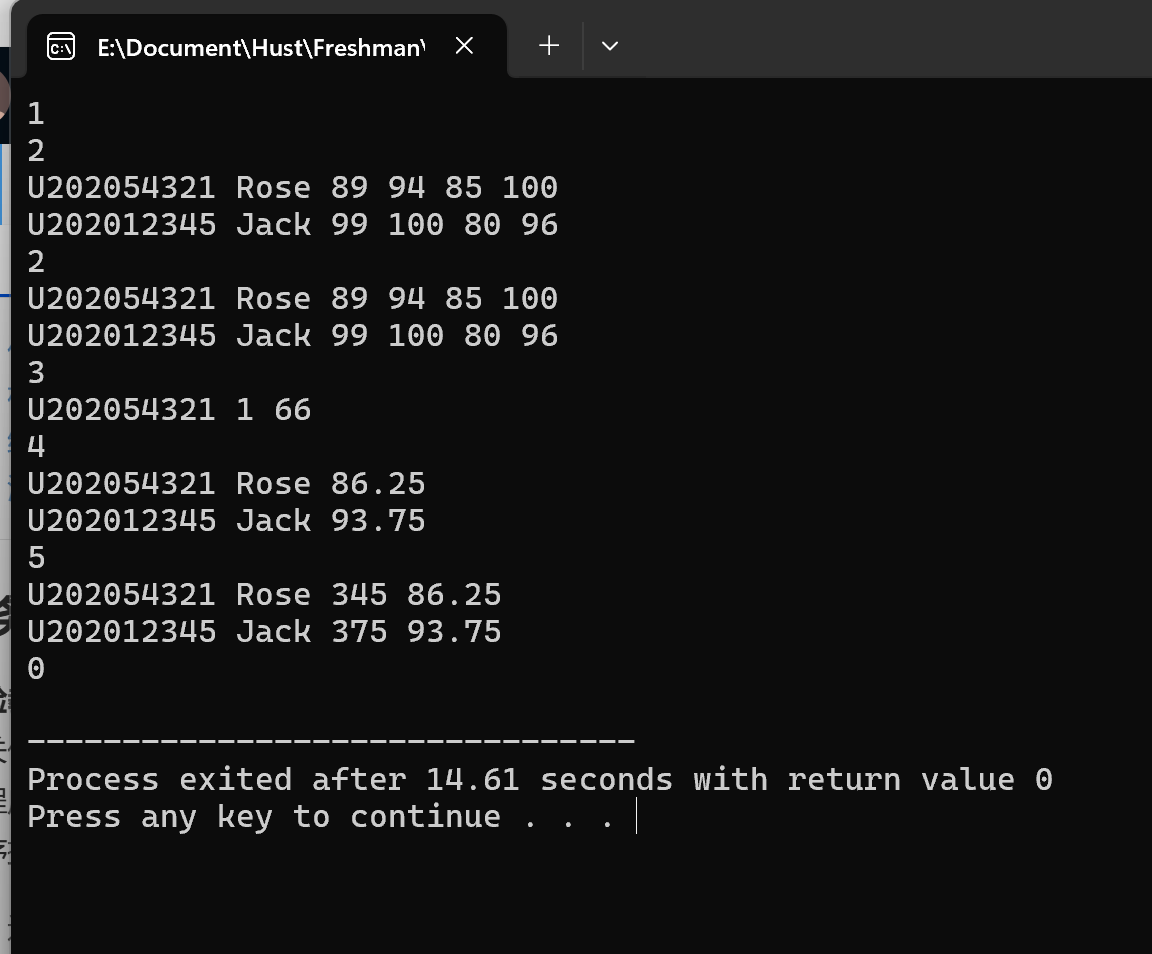
\includegraphics[scale=0.70]{images/7-6-2.png}
					\caption{执行示例}
					\label{pic7-6-2}
				\end{center}
			\end{figure}
			\begin{figure}[H]
			\begin{center}
				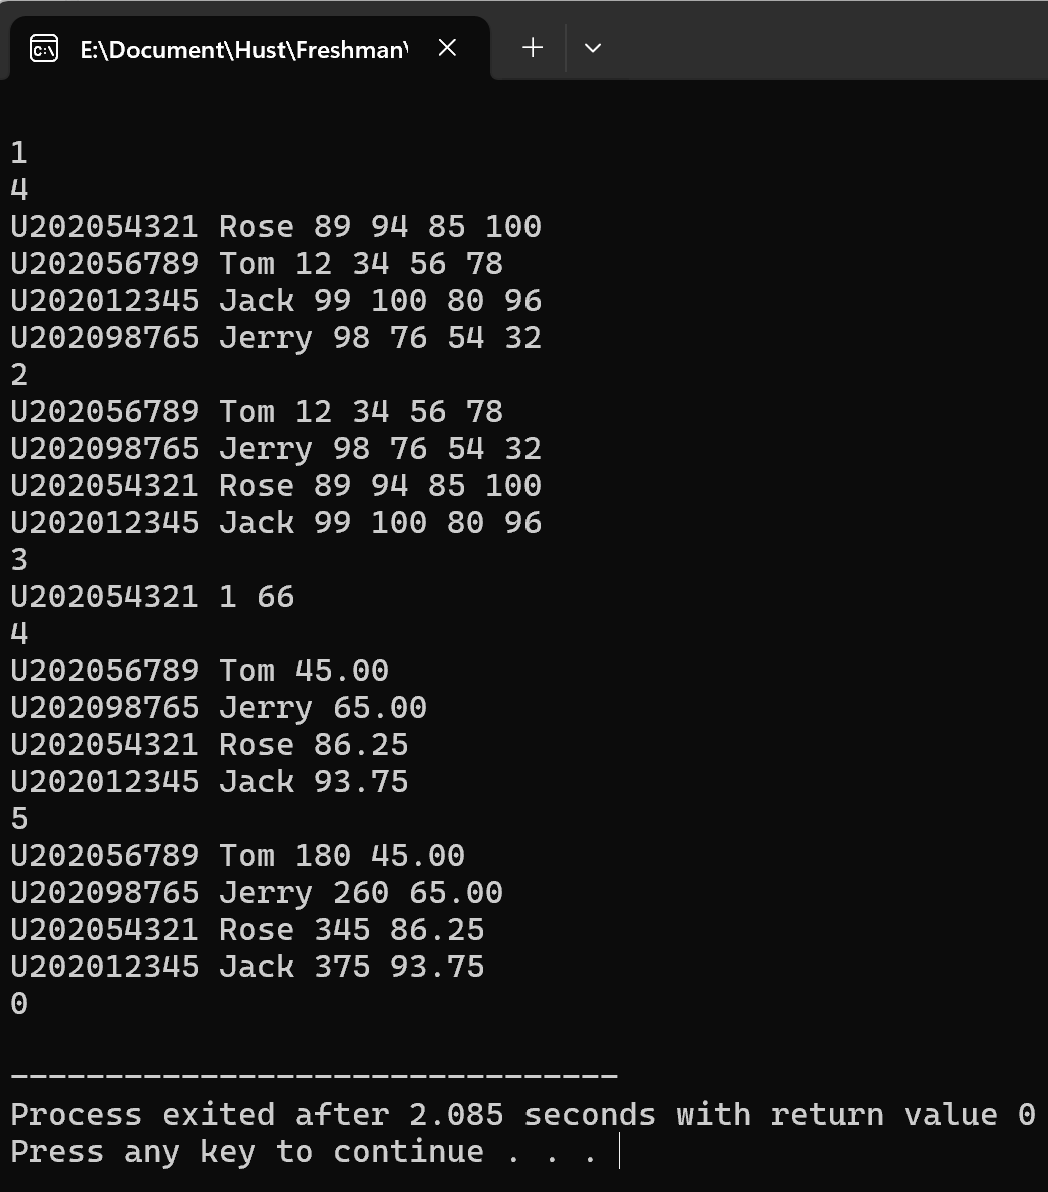
\includegraphics[scale=0.70]{images/7-6-3.png}
				\caption{执行示例}
				\label{pic7-6-3}
			\end{center}
		\end{figure}
\newpage
			\subsubsection{7-8 成绩排序（二）}
			\subsubsubsection{目标内容}
			对于程序设计第三题，进一步写出用交换结点指针域的方法升序排序的函数。
			\subsubsubsection{分析}
			采用交换节点指针域的方式来进行链表排序，同样可以选择如选择排序或冒泡排序的基本思想来实现升序排列。这里以选择排序为例进行说明，整体思路是每次遍历链表未排序部分，找到平均成绩最小的节点对应的指针，然后通过调整指针域，也就是改变节点之间的链接关系，将这个最小平均成绩的节点移动到已排序部分的末尾，然后经过多轮这样的操作，最终使得整个链表按照学生平均成绩升序排列。
			总流程图(\ref{pic7-5-1})：
			\begin{figure}[H]
				\begin{center}
					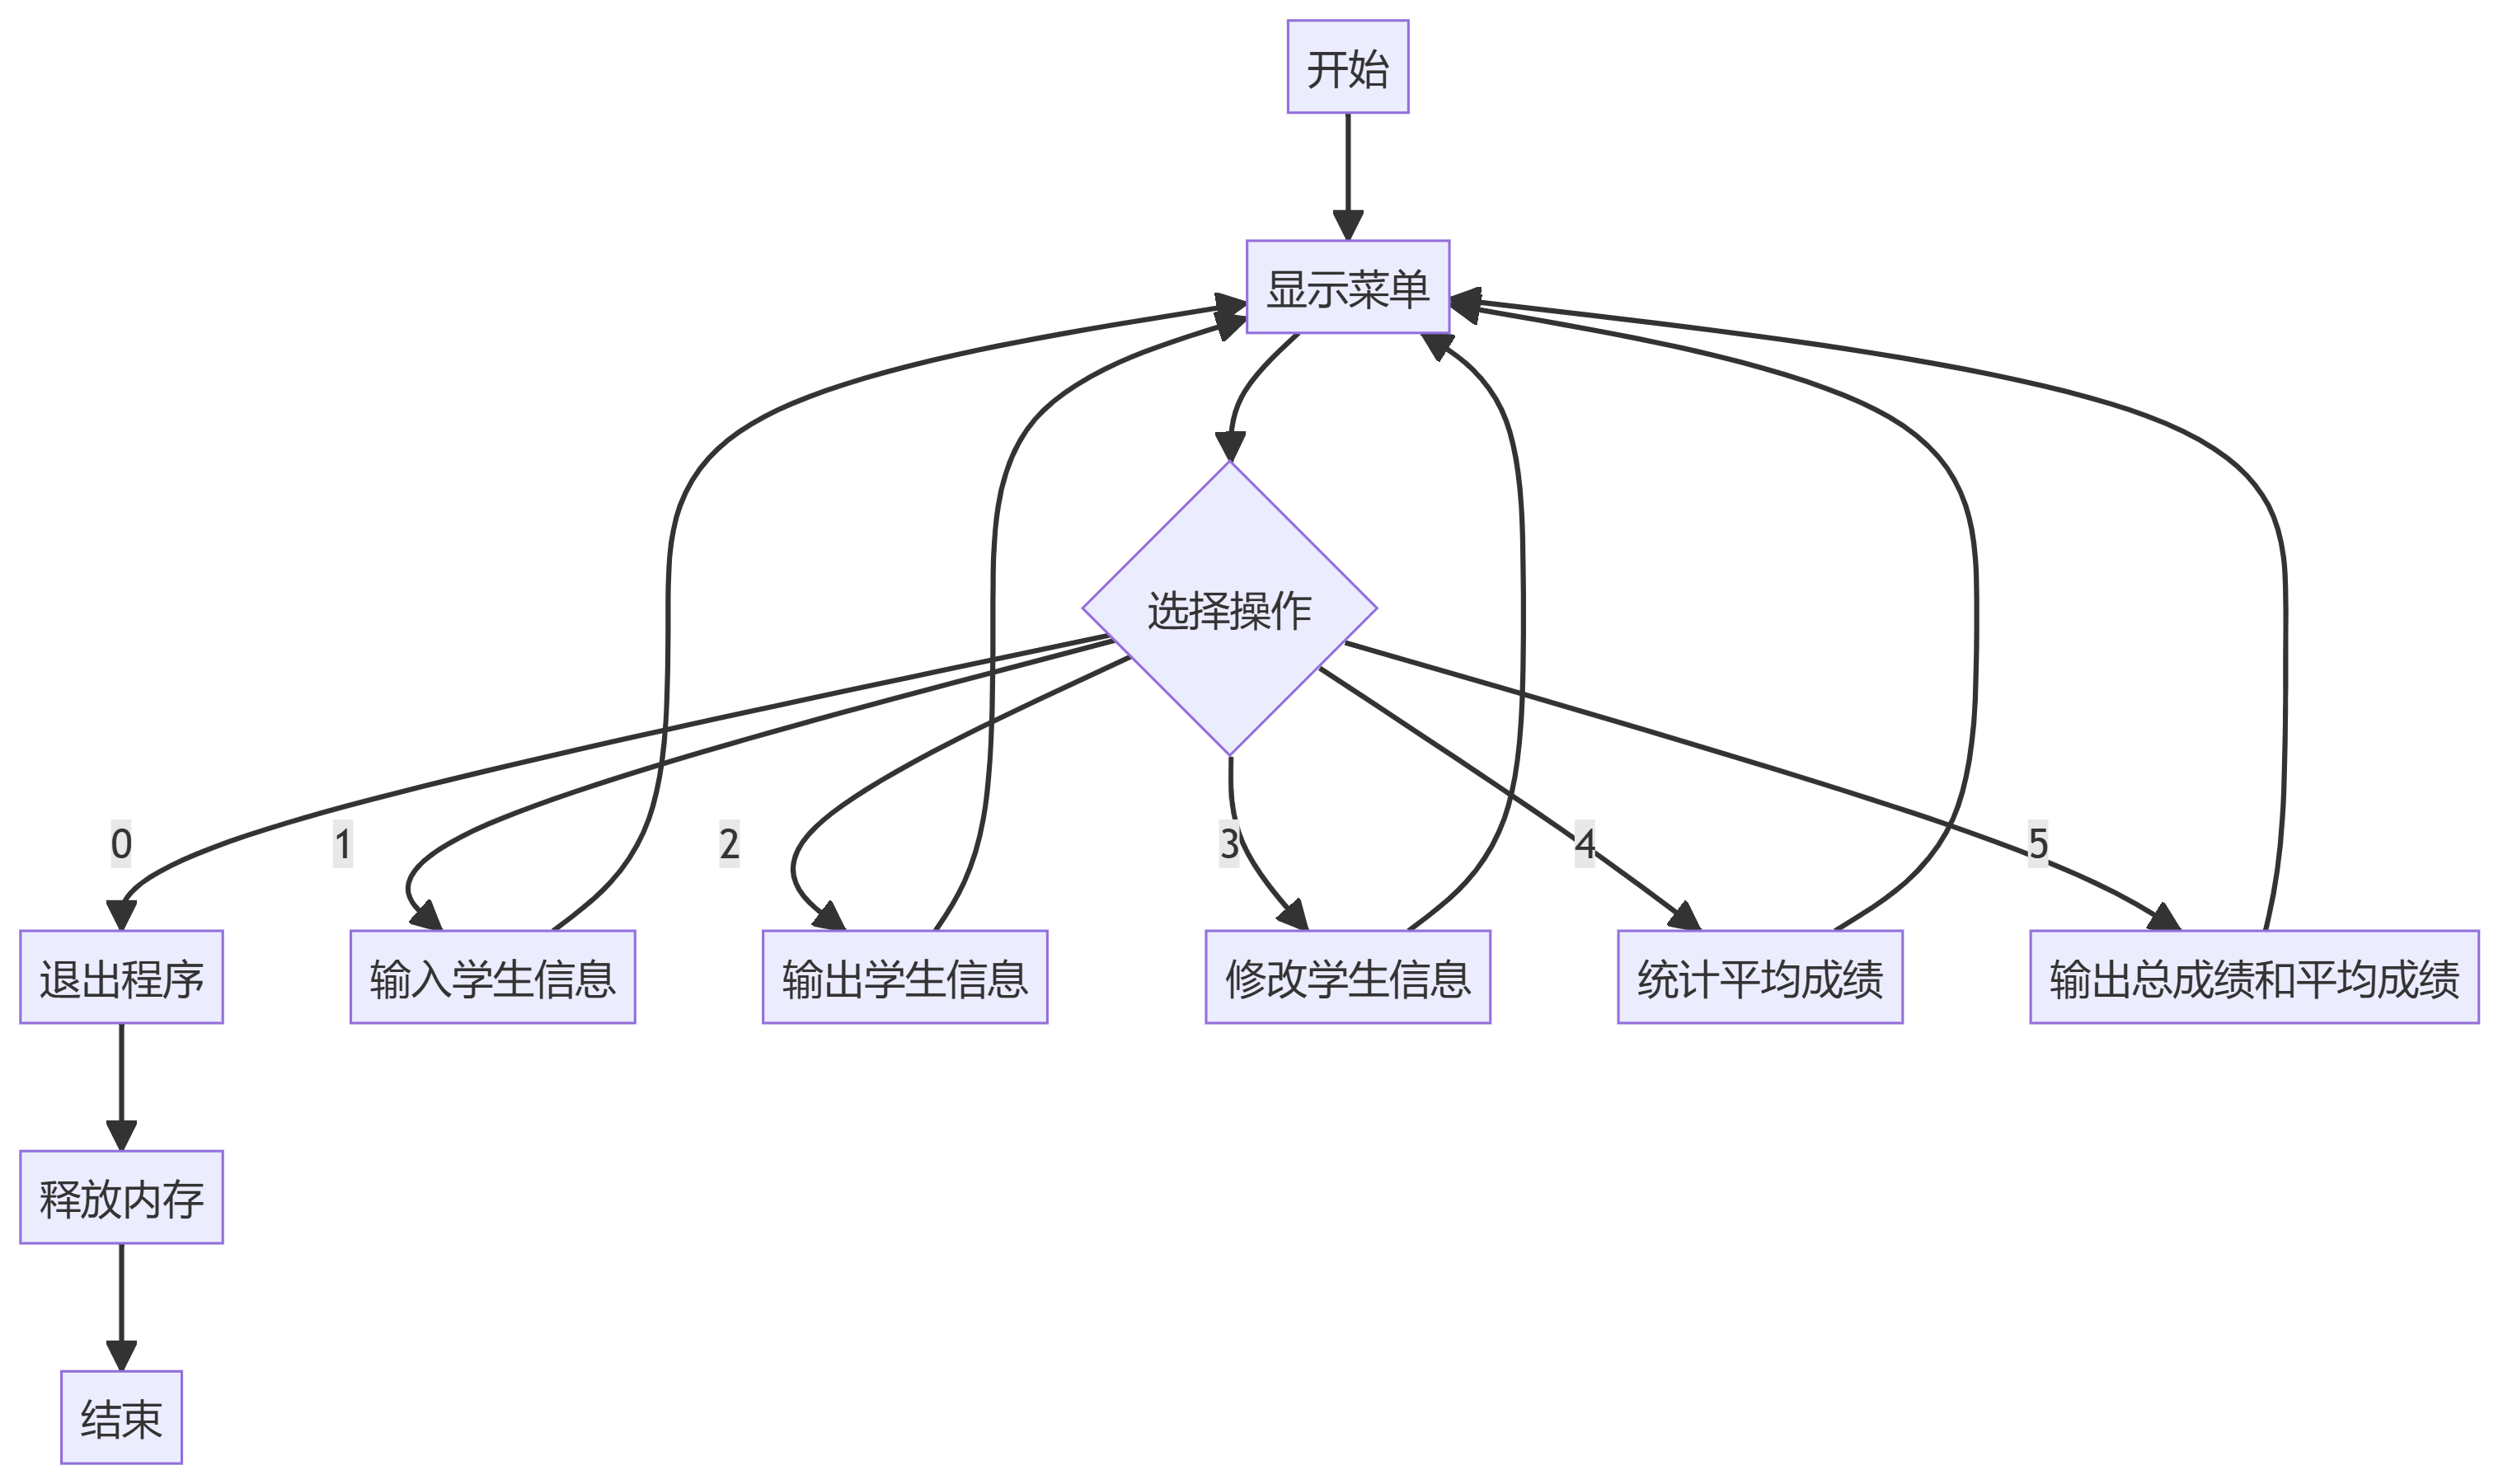
\includegraphics[scale=0.15]{images/7-5-1.png}
					\caption{总流程图}
					\label{pic7-5-1}
				\end{center}
			\end{figure}
			思路：\\
			    我们可以通过两层嵌套的循环来遍历链表，外层循环用于控制每一轮排序操作，确定当前已排序部分的末尾位置（也就是下一个要插入最小平均成绩节点的位置）；内层循环则从外层循环当前位置的下一个节点开始，遍历未排序部分的所有节点，比较各节点的平均成绩，记录下平均成绩最小的节点的指针。\\
			    而当找到未排序部分中平均成绩最小的节点指针后，需要调整指针域来改变节点顺序。具体来说，要将这个最小平均成绩节点从原来的位置 “脱离” 出来，并插入到当前已排序部分的末尾（即当前未排序部分的开头）。这涉及到修改相关节点的 next 指针，使得链表的链接关系按照平均成绩升序重新排列，而节点本身存储的学生数据（学号、姓名、各门课程成绩等）并没有进行交换，只是改变了链表中节点的顺序。
			
			相關流程图(\ref{pic7-8-3})
			\begin{figure}[H]
			\begin{center}
				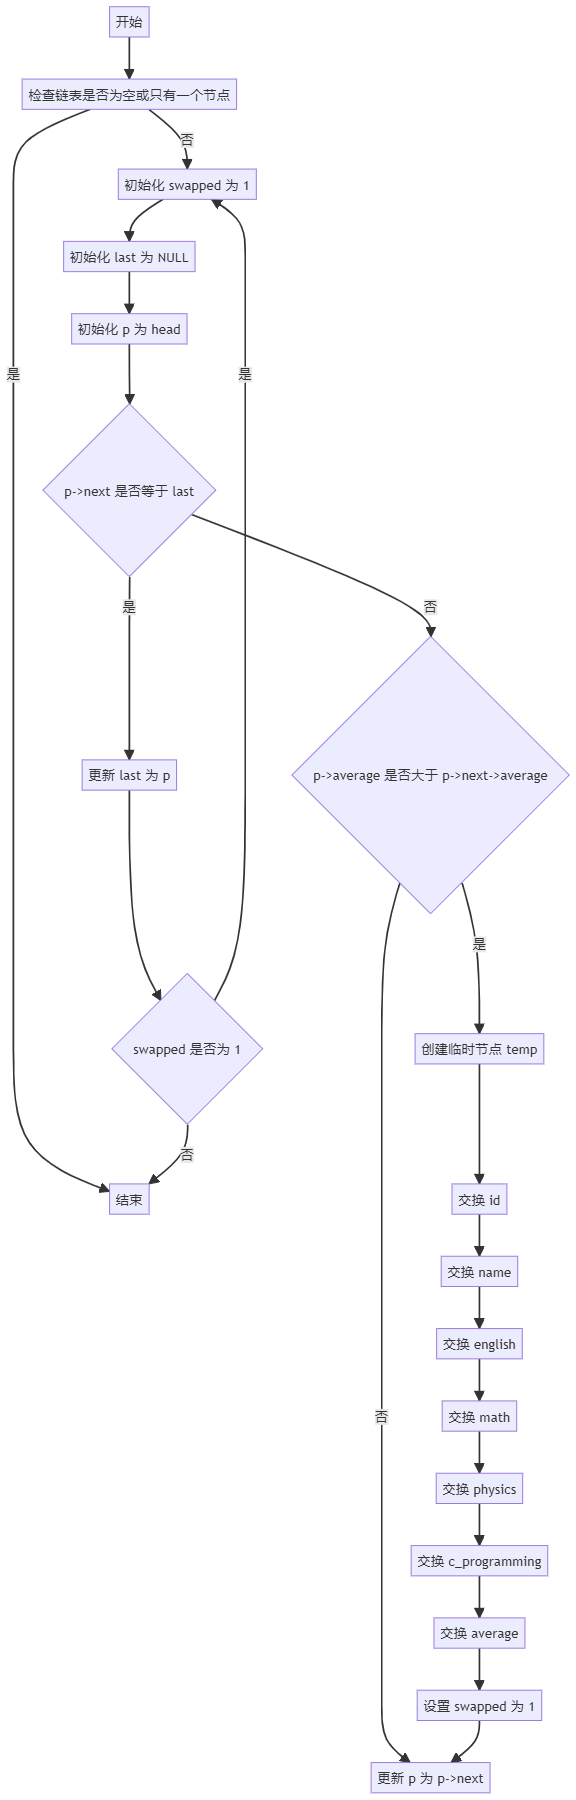
\includegraphics[scale=0.35]{images/7-8-3.png}
				\caption{流程图}
				\label{pic7-8-3}
			\end{center}
			\end{figure}
			
			\subsubsubsection{相关代码}
			\begin{lstlisting}[style=commonCodeStyle, caption={示例}, label={lst:7-8-1}]
				#include <stdio.h>
				#include <stdlib.h>
				#include <string.h>
				#include <math.h>
				#define NAME_LEN 50
				typedef struct Student {
					char id[20];
					char name[NAME_LEN];
					float english;
					float math;
					float physics;
					float c_programming;
					float average;
					struct Student *next;
				} Student;
				Student *createNode(char *id, char *name, float english, float math, float physics, float c_programming);
				void addStudent(Student **head, char *id, char *name, float english, float math, float physics, float c_programming);
				void printStudents(Student *head, int isAveragePrinted);
				void modifyStudent(Student *head, char *id, int choice, float newValue);
				void sortStudentsByAverage(Student **head);
				void printAverages(Student *head);
				void printTotalAndAverage(Student *head);
				Student *createNode(char *id, char *name, float english, float math, float physics, float c_programming) {
					Student *newNode = (Student *)malloc(sizeof(Student));
					if (newNode == NULL) {
						exit(1);
					}
					strcpy(newNode->id, id);
					strcpy(newNode->name, name);
					newNode->english = english;
					newNode->math = math;
					newNode->physics = physics;
					newNode->c_programming = c_programming;
					newNode->average = (english + math + physics + c_programming) / 4.0;
					newNode->next = NULL;
					return newNode;
				}
				void addStudent(Student **head, char *id, char *name, float english, float math, float physics, float c_programming) {
					Student *newNode = createNode(id, name, english, math, physics, c_programming);
					if (*head == NULL) {
						*head = newNode;
					}
					else {
						Student *temp = *head;
						while (temp->next!= NULL) {
							temp = temp->next;
						}
						temp->next = newNode;
					}
				}
				void printStudents(Student *head, int isAveragePrinted) {
					Student *temp = head;
					while (temp!= NULL) {
						printf("%s %s ", temp->id, temp->name);
						if (isAveragePrinted) {
							printf("%.2f ", temp->english);
							printf("%.2f ", temp->math);
							printf("%.2f ", temp->physics);
							printf("%.2f\n", temp->c_programming);
						}
						else {
							if ((int)temp->english == temp->english) {
								printf("%d ", (int)temp->english);
							}
							else {
								printf("%.2f ", temp->english);
							}
							if ((int)temp->math == temp->math) {
								printf("%d ", (int)temp->math);
							}
							else {
								printf("%.2f ", temp->math);
							}
							if ((int)temp->physics == temp->physics) {
								printf("%d ", (int)temp->physics);
							}
							else {
								printf("%.2f ", temp->physics);
							}
							if ((int)temp->c_programming == temp->c_programming) {
								printf("%d\n", (int)temp->c_programming);
							}
							else {
								printf("%.2f\n", temp->c_programming);
							}
						}
						temp = temp->next;
					}
				}
				void modifyStudent(Student *head, char *id, int choice, float newValue) {
					Student *temp = head;
					while (temp!= NULL) {
						if (strcmp(temp->id, id) == 0) {
							switch (choice) {
								case 1:
								temp->english = newValue;
								break;
								case 2:
								temp->math = newValue;
								break;
								case 3:
								temp->physics = newValue;
								break;
								case 4:
								temp->c_programming = newValue;
								break;
							}
							temp->average = (temp->english + temp->math + temp->physics + temp->c_programming) / 4.0;
							return;
						}
						temp = temp->next;
					}
				}
				void sortStudentsByAverage(Student **head) {
					if (*head == NULL || (*head)->next == NULL) {
						return;
					}
					Student *p;
					Student *last = NULL;
					int swapped;
					do {
						swapped = 0;
						p = *head;
						while (p->next!= last) {
							if (p->average > p->next->average) {
								Student temp;
								strcpy(temp.id, p->id);
								strcpy(p->id, p->next->id);
								strcpy(p->next->id, temp.id);
								strcpy(temp.name, p->name);
								strcpy(p->name, p->next->name);
								strcpy(p->next->name, temp.name);
								temp.english = p->english;
								p->english = p->next->english;
								p->next->english = temp.english;
								temp.math = p->math;
								p->math = p->next->math;
								p->next->math = temp.math;
								temp.physics = p->physics;
								p->physics = p->next->physics;
								p->next->physics = temp.physics;
								temp.c_programming = p->c_programming;
								p->c_programming = p->next->c_programming;
								p->next->c_programming = temp.c_programming;
								temp.average = p->average;
								p->average = p->next->average;
								p->next->average = temp.average;
								swapped = 1;
							}
							p = p->next;
						}
						last = p;
					} while (swapped);
				}
				void printAverages(Student *head) {
					Student *temp = head;
					while (temp!= NULL) {
						printf("%s %s %.2f\n", temp->id, temp->name, temp->average);
						temp = temp->next;
					}
				}
				void printTotalAndAverage(Student *head) {
					Student *temp = head;
					while (temp!= NULL) {
						float total = temp->english + temp->math + temp->physics + temp->c_programming;
						printf("%s %s %d %.2f\n", temp->id, temp->name, (int)total, temp->average);
						temp = temp->next;
					}
				}
				int main() {
					Student *head = NULL;
					int choice, n;
					char id[20], name[NAME_LEN];
					float english, math, physics, c_programming;
					char modifyId[20];
					int modifyChoice;
					float newValue;
					int isAveragePrinted = 0;
					while (1) {
						scanf("%d", &choice);
						
						switch (choice) {
							case 0:
							while (head!= NULL) {
								Student *temp = head;
								head = head->next;
								free(temp);
							}
							exit(0);
							case 1:
							scanf("%d", &n);
							for (int i = 0; i < n; i++) {
								scanf("%s %s %f %f %f %f", id, name, &english, &math, &physics, &c_programming);
								addStudent(&head, id, name, english, math, physics, c_programming);
							}
							break;
							case 2:
							sortStudentsByAverage(&head);
							printStudents(head, isAveragePrinted);
							break;
							case 3:
							scanf("%s %d %f", modifyId, &modifyChoice, &newValue);
							modifyStudent(head, modifyId, modifyChoice, newValue);
							break;
							case 4:
							sortStudentsByAverage(&head); 
							printAverages(head);
							isAveragePrinted = 1;
							break;
							case 5:
							sortStudentsByAverage(&head);
							printTotalAndAverage(head);
							break;
						}
					}
					return 0;
				}
			\end{lstlisting}
			
			\subsubsubsection{执行结果}
			执行结果(\ref{\ref{pic7-8-1}}\ref{pic7-8-2})：
			\begin{figure}[H]
				\begin{center}
					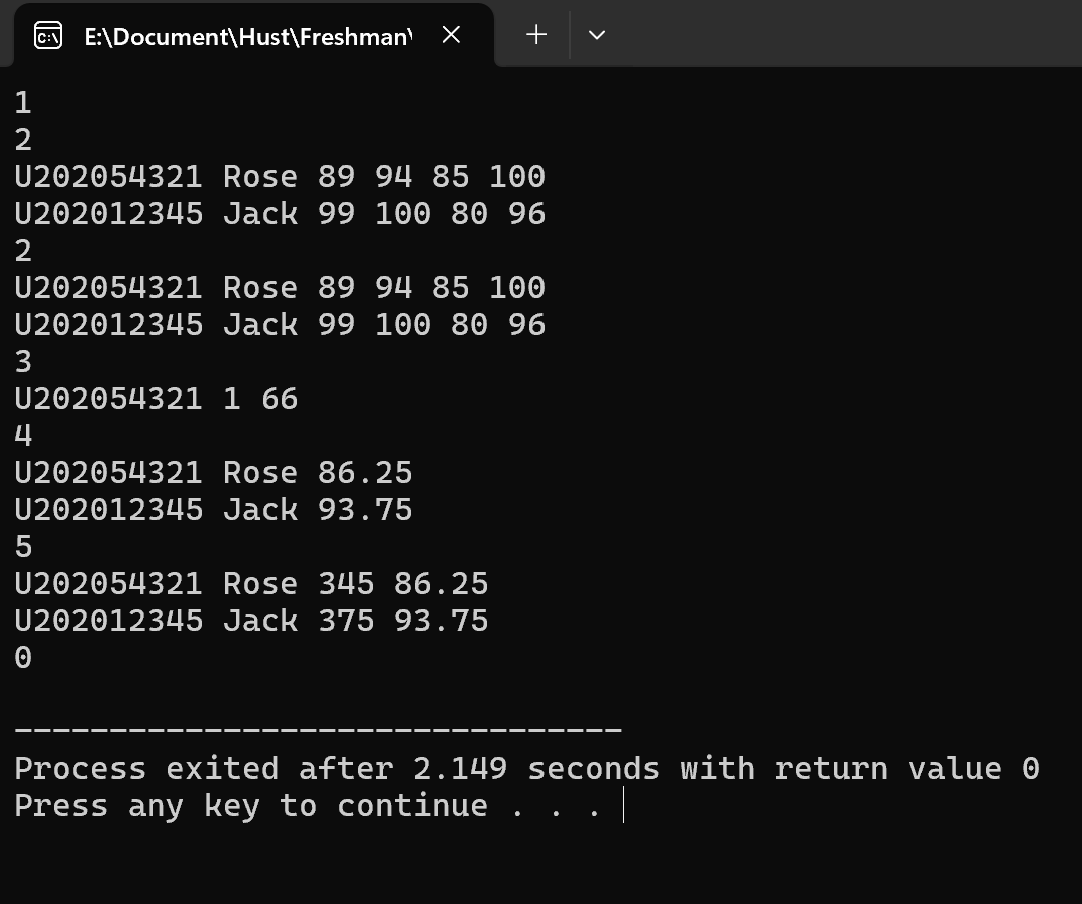
\includegraphics[scale=0.50]{images/7-8-1.png}
					\caption{执行示例}
					\label{pic7-8-1}
				\end{center}
			\end{figure}
			\begin{figure}[H]
				\begin{center}
					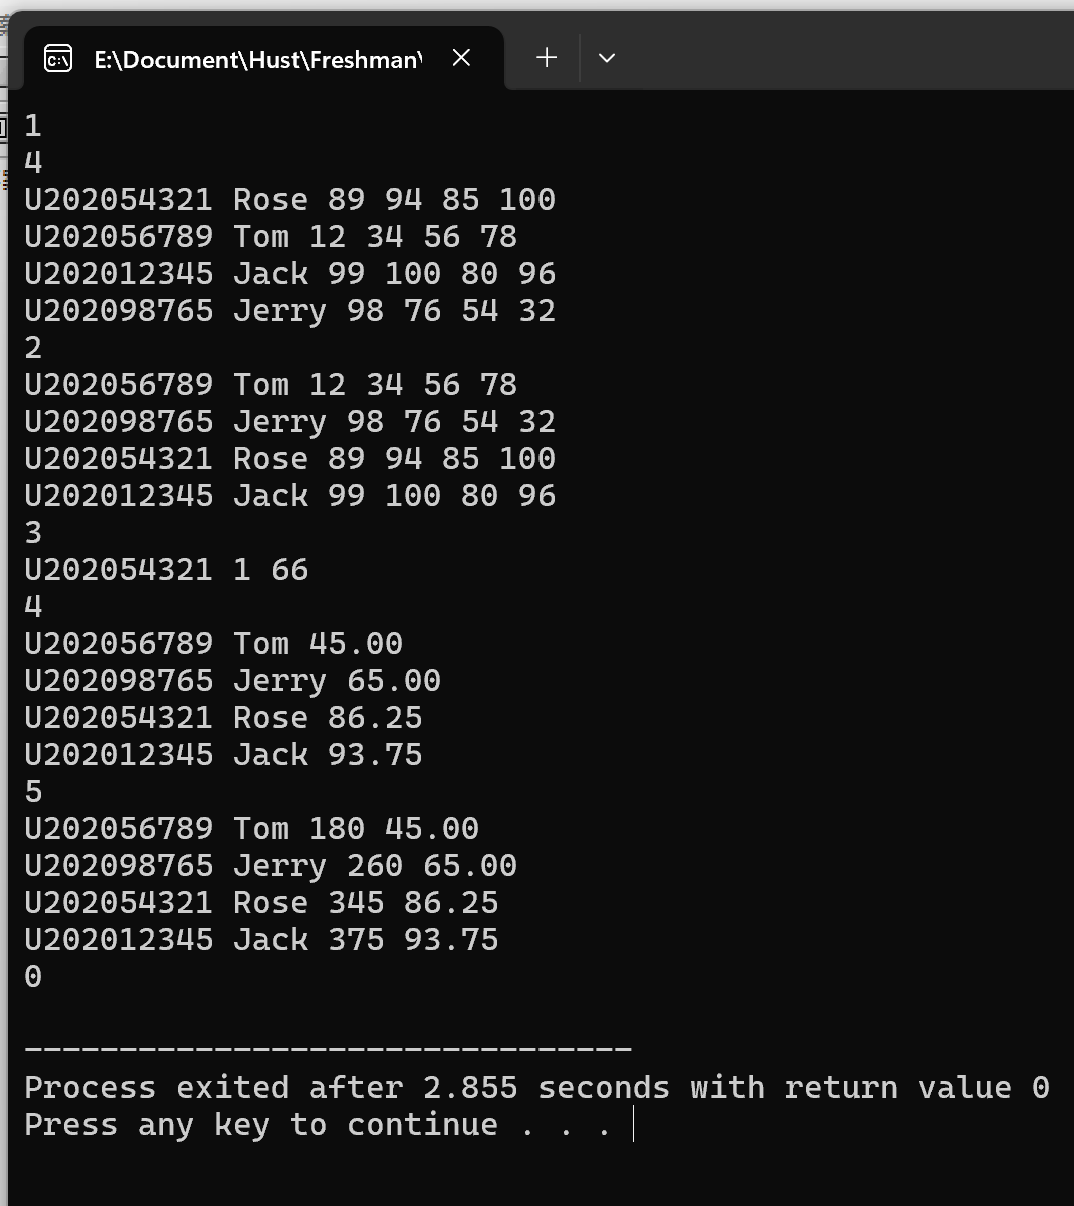
\includegraphics[scale=0.50]{images/7-8-2.png}
					\caption{执行示例}
					\label{pic7-8-2}
				\end{center}
			\end{figure}
\newpage
			\subsubsection{7-7 回文字符串}
			\subsubsubsection{目标内容}
			回文字符串是正读和反读都相同的字符串，例如“abba”和“abcba”是回文字符串。设计程序判断输入的任意长度的字符串是否为回文字符串。
			提示：由于要求字符串长度任意，所以用单链表存储字符串，即判断一个单链表是否为回文链表。
			\subsubsubsection{分析}
			我们需要设计一个程序来判断一个单链表存储的字符串是否为回文字符串。回文字符串是指正读和反读都相同的字符串，例如 "abba" 和 "abcba"。\\
			总流程图(\ref{pic7-7-1})：
			\begin{figure}[H]
				\begin{center}
					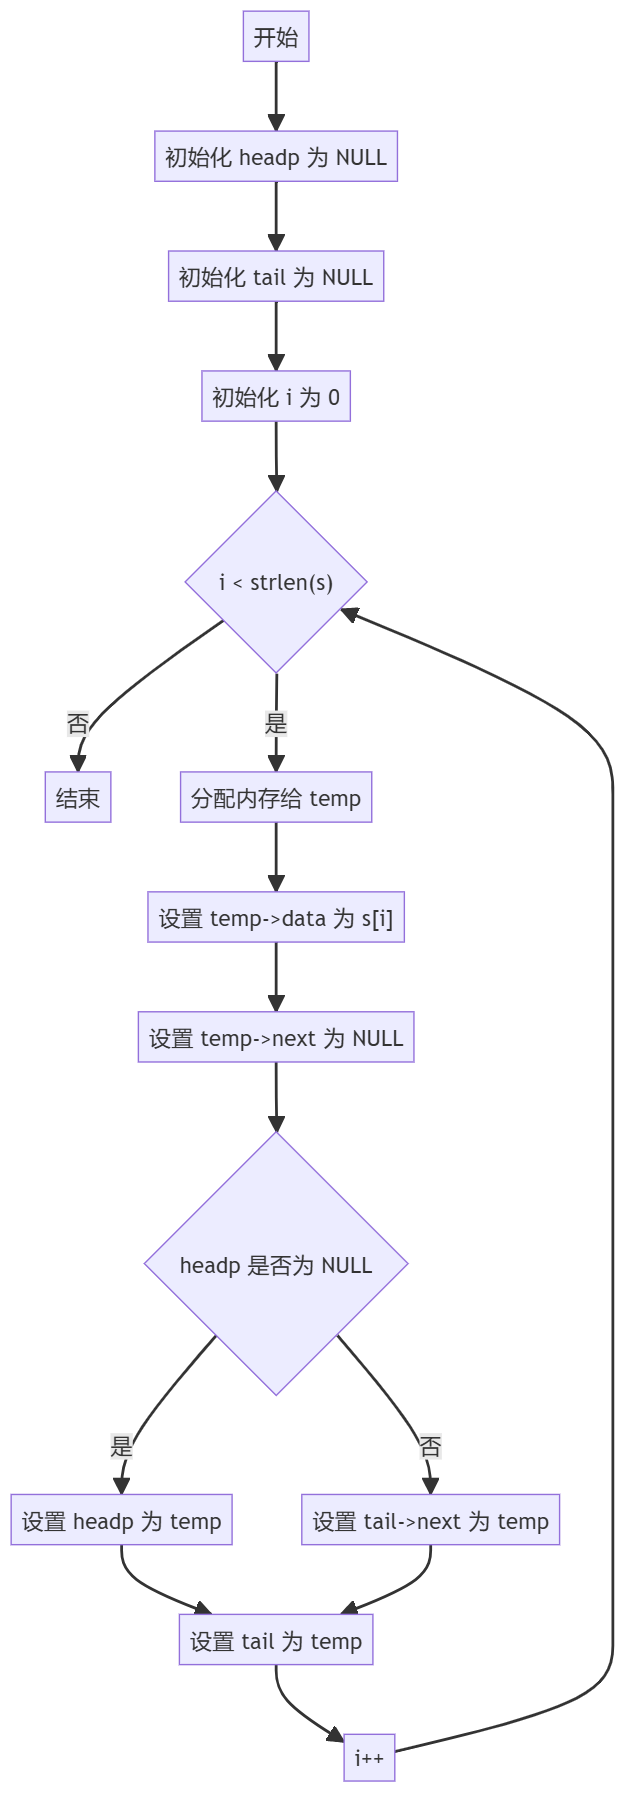
\includegraphics[scale=0.33]{images/7-7-1.png}
					\caption{总流程图}
					\label{pic7-7-1}
				\end{center}
			\end{figure}
			思路：\\
			选用单链表来存储字符串是因为题目要求能处理任意长度的字符串，单链表具有动态分配内存的特点，可以根据字符串的实际长度灵活地创建相应数量的节点来存储字符，避免了像数组那样需要预先指定固定大小可能导致空间浪费或者不够用的问题。\\
			流程图(\ref{pic7-7-2})：
			\begin{figure}[H]
				\begin{center}
					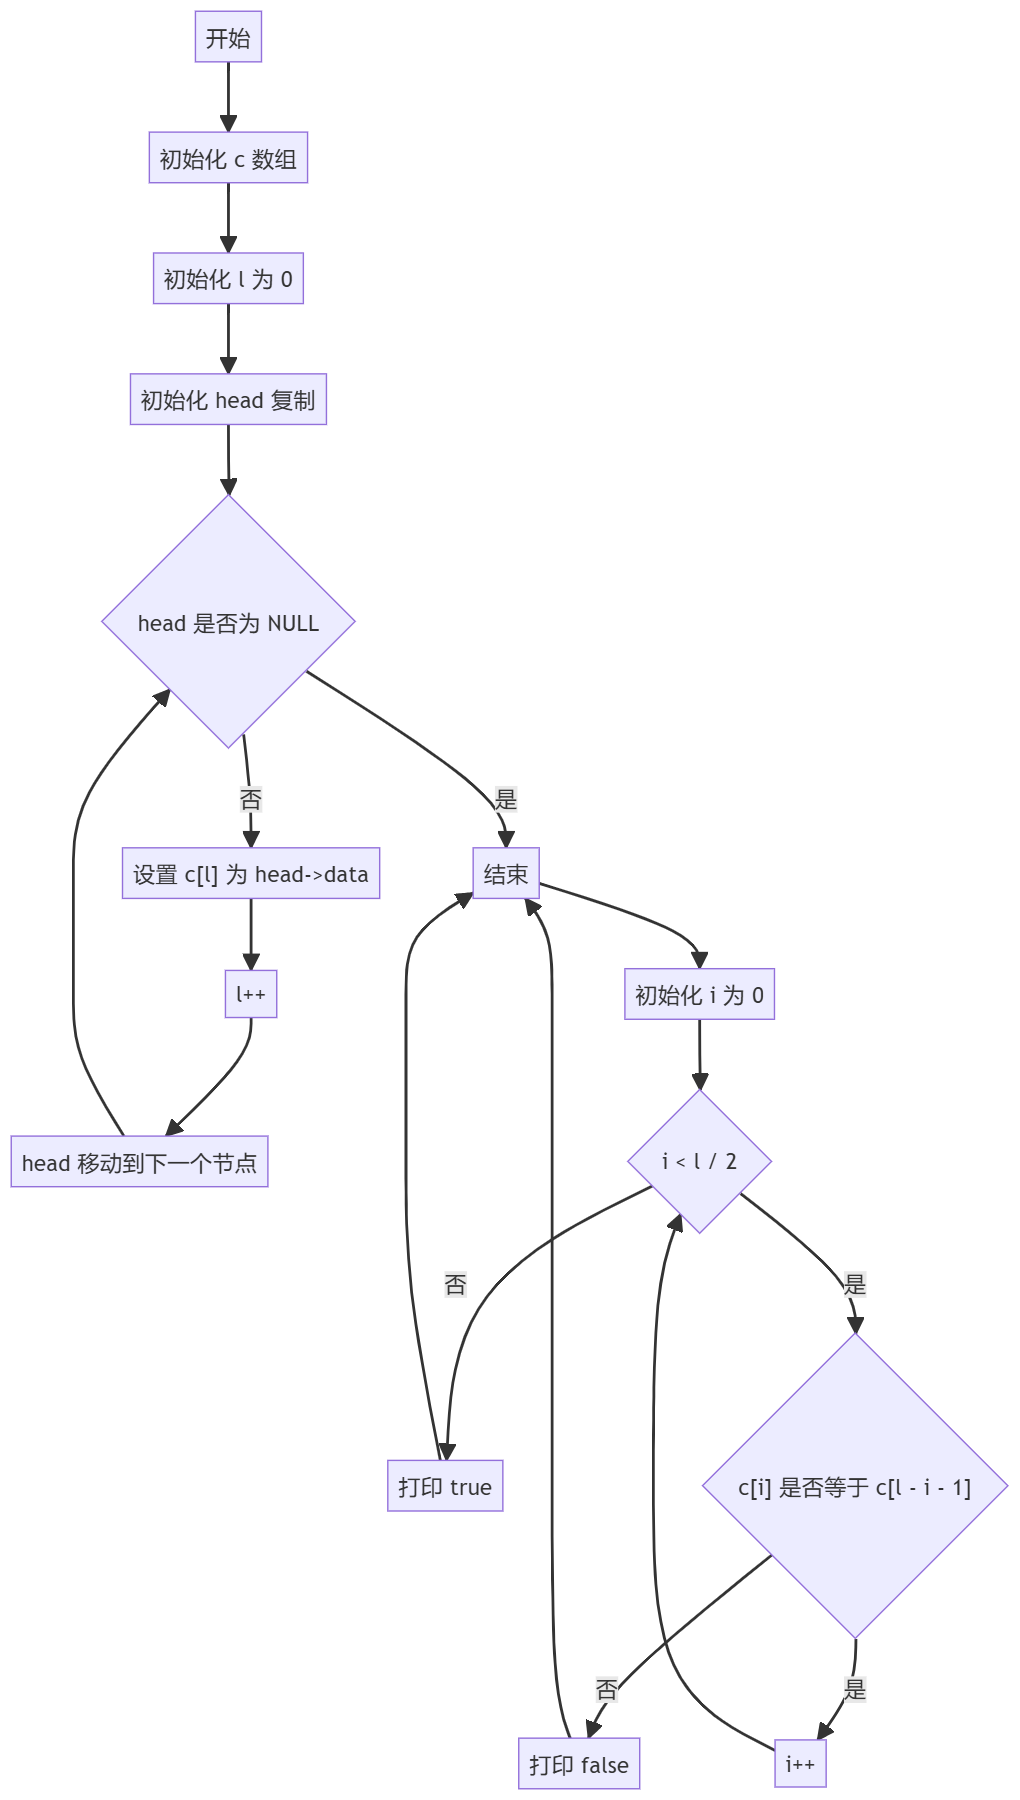
\includegraphics[scale=0.34]{images/7-7-2.png}
					\caption{流程图}
					\label{pic7-7-2}
				\end{center}
			\end{figure}
			
			\subsubsubsection{相关代码}
			相关代码(\ref{lst:7-7-1})：
			\begin{lstlisting}[style=commonCodeStyle, caption={示例}, label={lst:7-7-1}]
				#include <stdio.h>
				#include <stdlib.h>
				#include <string.h>
				typedef struct C_NODE {
					char data;
					struct C_NODE *next;
				} C_NODE;
				void createLinkList(C_NODE **headp, char s[]) 
				{
					C_NODE *tail;
					*headp = NULL;
					tail = NULL;
					for(int i = 0; i < strlen(s); i++) {
						C_NODE *temp = (C_NODE *)malloc(sizeof(C_NODE));
						temp->data = s[i];
						temp->next = NULL;
						if (*headp == NULL) {
							*headp = temp; 
						} else {
							tail->next = temp; 
						}
						tail = temp; 
					}
				}
				void judgePalindrome(C_NODE *head)
				{
					char c[1000];
					int l = 0;
					while(head != NULL) {
						c[l++] = head->data;
						head = head->next;
					}
					for (int i = 0; i < l / 2; i++) {
						if (c[i] != c[l - i - 1]) {
							printf("false\n");
							return;
						}
					}
					printf("true\n");
				}
				int main() {
					C_NODE *head = NULL;
					char inputString[1000];
					fgets(inputString, sizeof(inputString), stdin);
					size_t len = strlen(inputString);
					if (len > 0 && inputString[len - 1] == '\n') {
						inputString[len - 1] = '\0';
					}
					createLinkList(&head, inputString);
					judgePalindrome(head);
					C_NODE *current = head;
					while (current != NULL) {
						C_NODE *next = current->next;
						free(current);
						current = next;
					}
					return 0;
				}
			\end{lstlisting}
			
			\subsubsubsection{执行结果}
			执行结果(\ref{pic7-7-3}\ref{pic7-7-4})：
			\begin{figure}[H]
				\begin{center}
					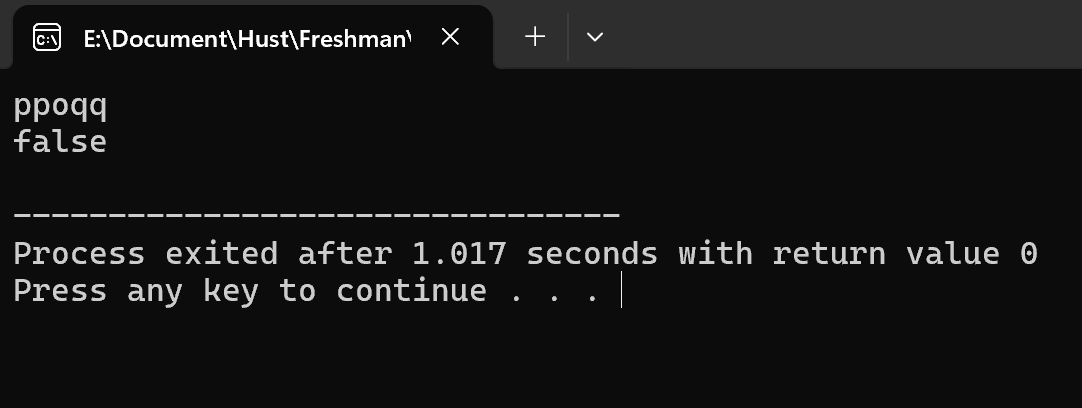
\includegraphics[scale=0.70]{images/7-7-3.png}
					\caption{执行示例}
					\label{pic7-7-3}
				\end{center}
			\end{figure}
			\begin{figure}[H]
				\begin{center}
					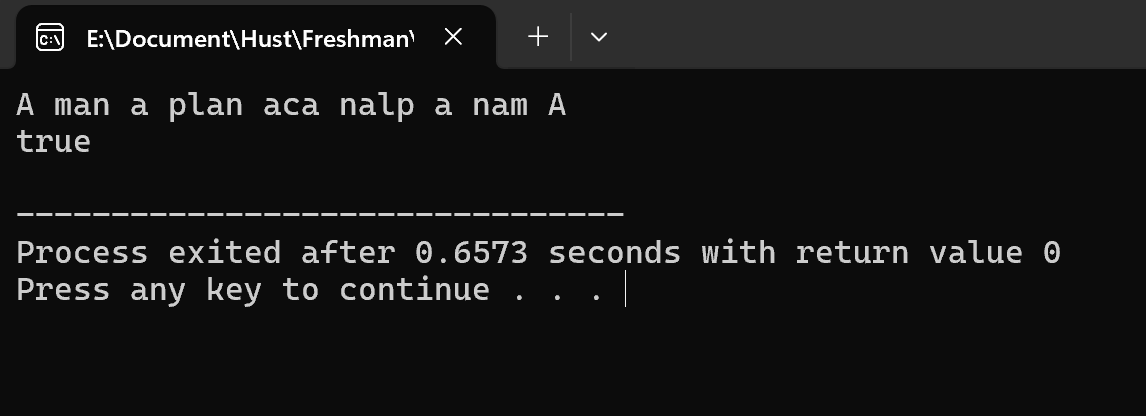
\includegraphics[scale=0.70]{images/7-7-4.png}
					\caption{执行示例}
					\label{pic7-7-4}
				\end{center}
			\end{figure}
		可见通过上述的分析兴代码实现，构建了这个能识别回文的程序。
			
			\subsubsection{逆波兰表达式}
			\subsubsubsection{目标内容}
			利用值栈对逆波兰表达式进行求值。逆波兰表达式从键盘输入，其中的运算符仅包含加、减、乘、除4种运算，表达式中的数都是十进制数，用换行符结束输入。由于逆波兰表达式的长度不限，所以值栈要用后进先出链表实现。
			\subsubsubsection{分析}
			本题旨在解决对从键盘输入的逆波兰表达式进行求值的问题。由于逆波兰表达式长度不限，所以采用后进先出链表来实现值栈，以适应不同长度表达式的计算需求，并且限定表达式中的运算符为加、减、乘、除四种基本运算，操作数为十进制数，通过栈操作和运算逻辑来得出最终的表达式求值结果。
			总流程图(\ref{pic7-9-1})：
			\begin{figure}[H]
				\begin{center}
					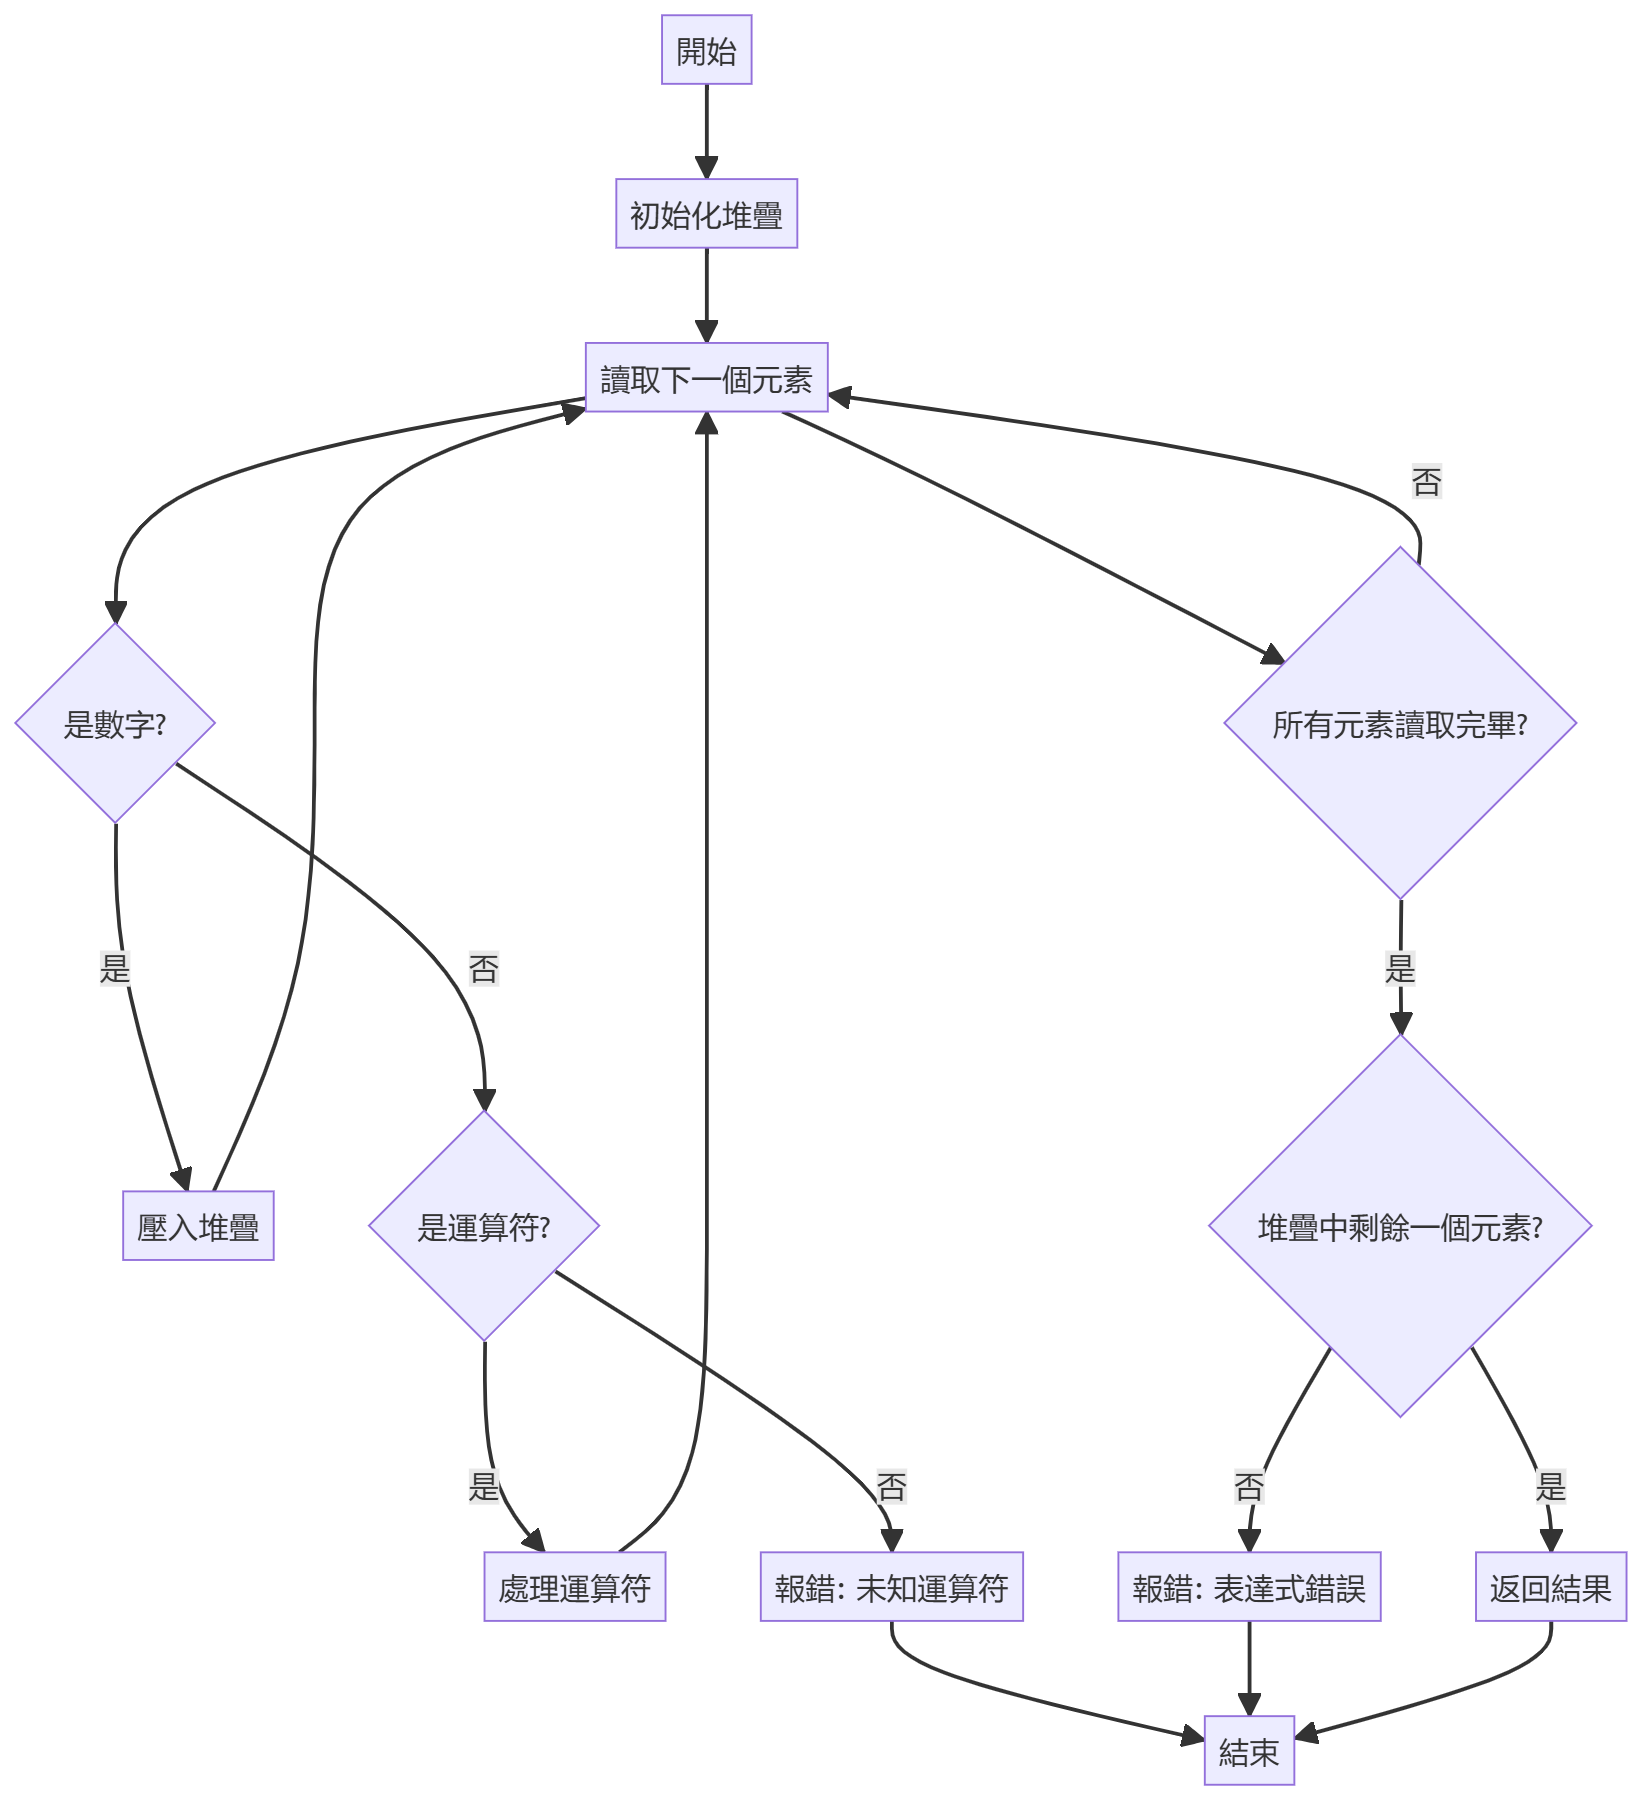
\includegraphics[scale=0.20]{images/7-9-1.png}
					\caption{总流程图}
					\label{pic7-9-1}
				\end{center}
			\end{figure}
			思路：\\
			本程序基于逆波兰表达式求值特点，选用后进先出链表实现值栈来构建求值程序。因逆波兰表达式计算顺序契合栈的后进先出特性且长度不限，链表可动态分配内存适应需求，故以链表实现栈。
			在 void 函数中，初始化栈顶指针为 NULL，按输入顺序处理元素，操作数入栈，运算符则弹出操作数计算后将结果入栈，处理完所有元素后根据栈状态确定求值结果并处理错误情况，最后在 main 函数中调用 void函数求值并输出结果。
			相关流程图(\ref{pic7-9-2})：
			\begin{figure}[H]
				\begin{center}
					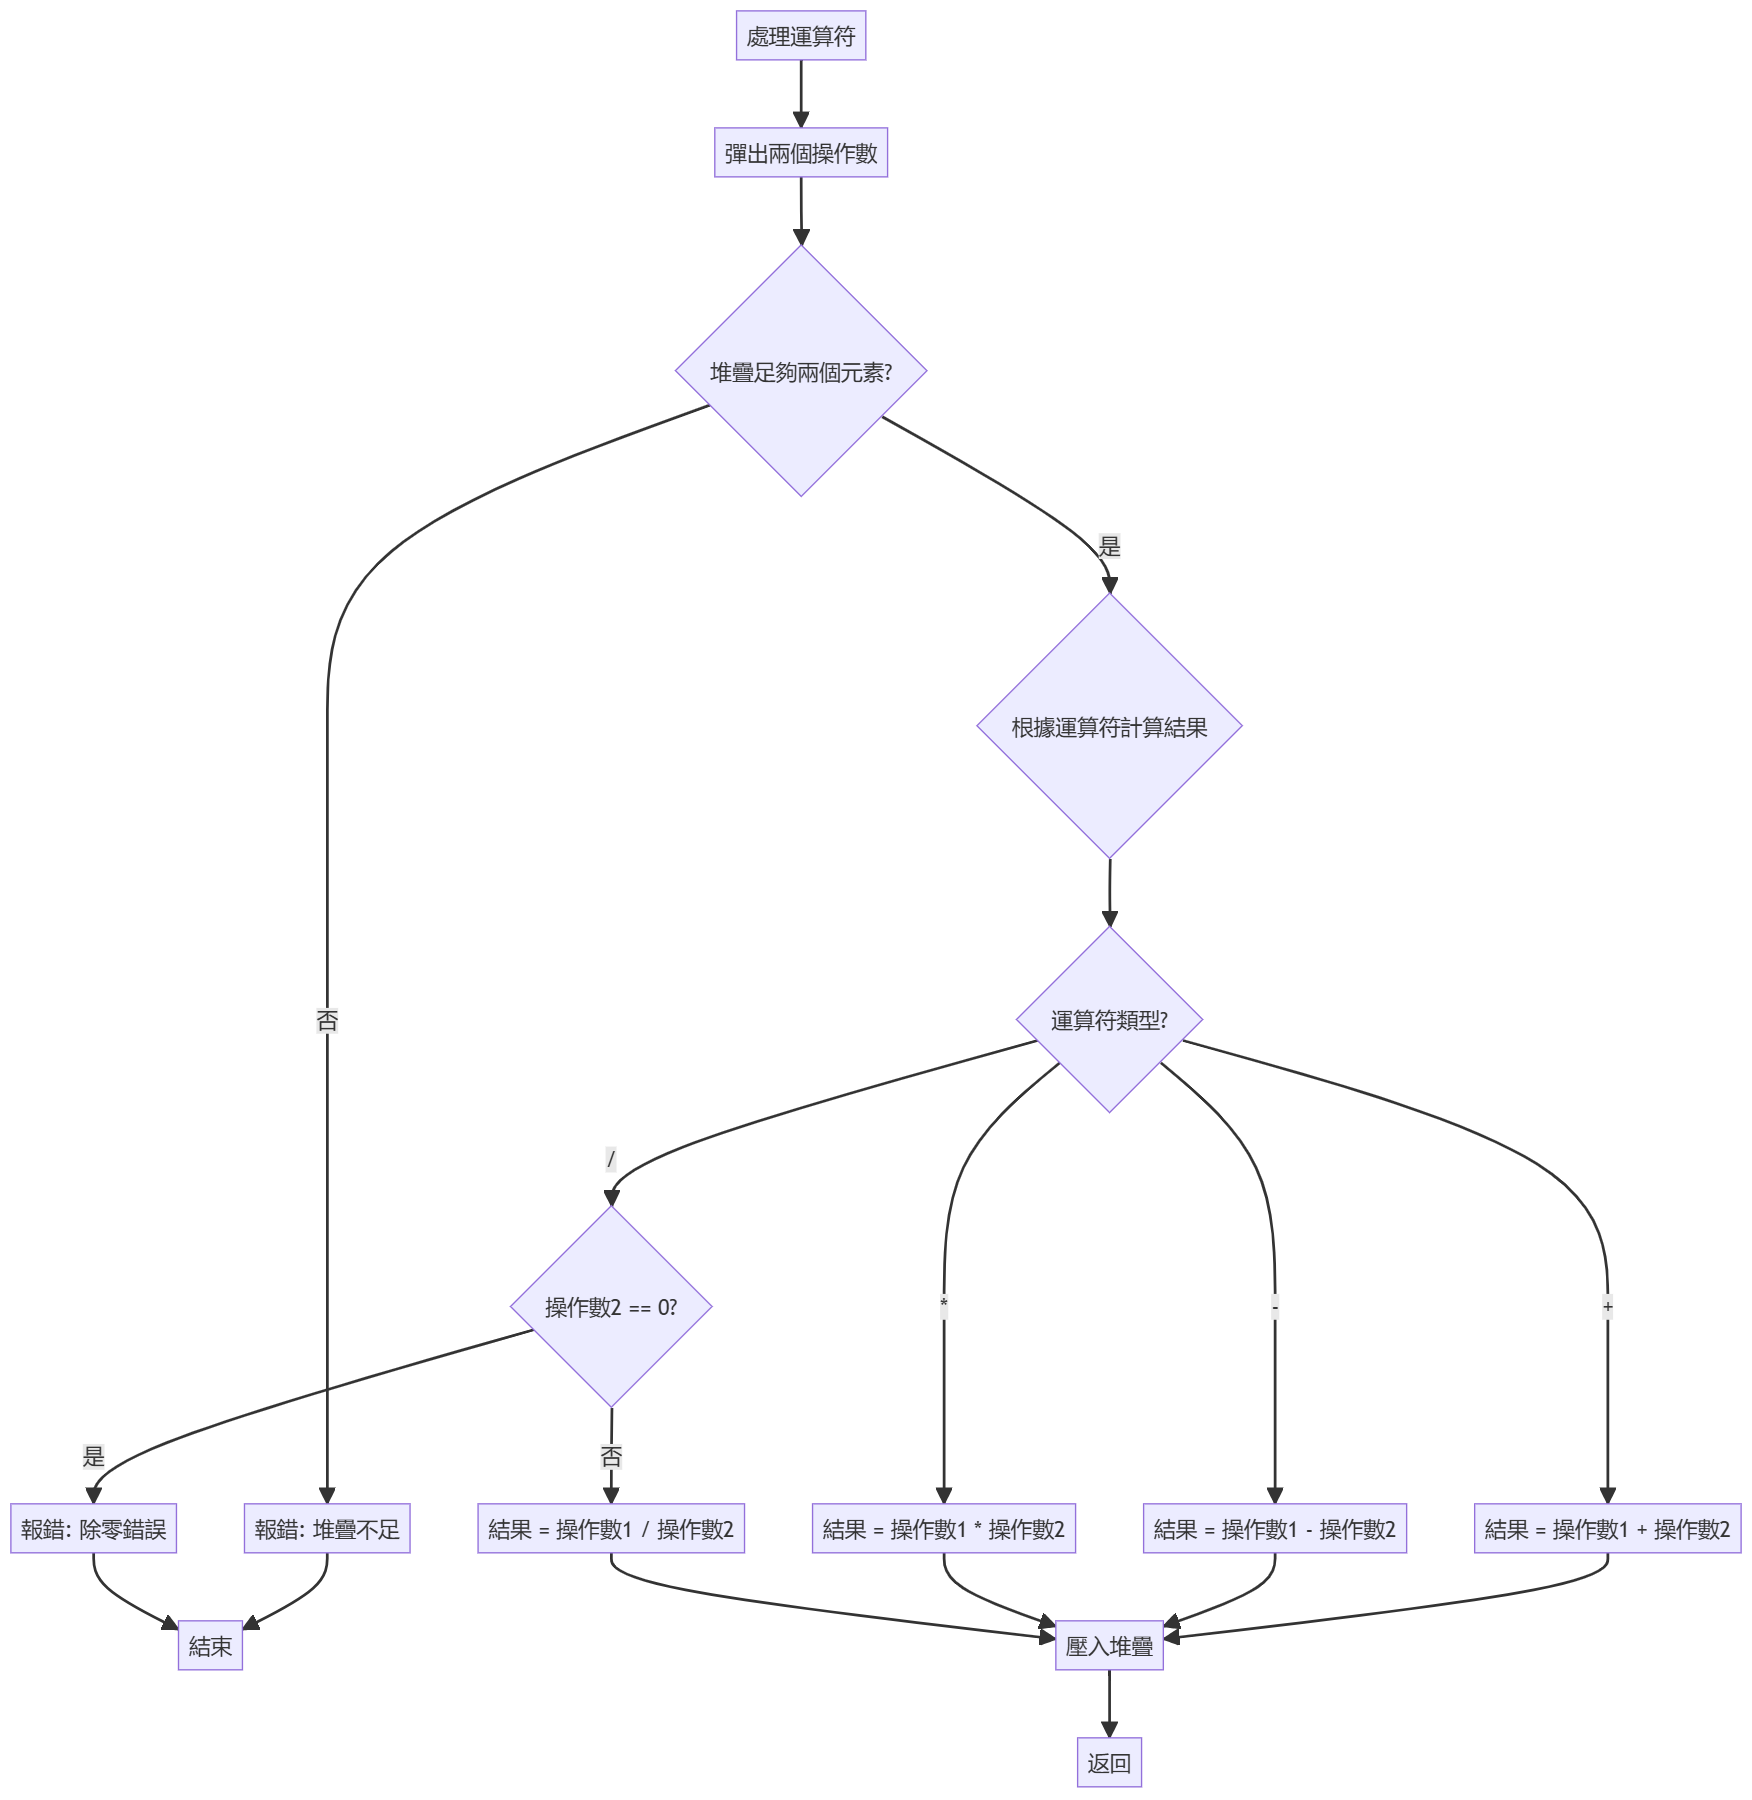
\includegraphics[scale=0.23]{images/7-9-2.png}
					\caption{流程图}
					\label{pic7-9-2}
				\end{center}
			\end{figure}
			
			
			\subsubsubsection{相关代码}
			相关代码(\ref{lst:7-9-1})：
			\begin{lstlisting}[style=commonCodeStyle, caption={示例}, label={lst:7-9-1}]
				#include <stdio.h>
				#include <stdlib.h>
				#include <ctype.h>
				#include <string.h>
				typedef struct StackNode {
					float value;
					struct StackNode *next;
				} StackNode;
				StackNode *createNode(float value) {
					StackNode *newNode = (StackNode *)malloc(sizeof(StackNode));
					if (newNode == NULL) {
						fprintf(stderr, "内存分配失败\n");
						exit(1);
					}
					newNode->value = value;
					newNode->next = NULL;
					return newNode;
				}
				void push(StackNode **top, float value) {
					StackNode *newNode = createNode(value);
					newNode->next = *top;
					*top = newNode;
				}
				float pop(StackNode **top) {
					if (*top == NULL) {
						fprintf(stderr, "栈为空\n");
						exit(1);
					}
					StackNode *temp = *top;
					float value = temp->value;
					*top = (*top)->next;
					free(temp);
					return value;
				}
				int isEmpty(StackNode *top) {
					return top == NULL;
				}
				float evaluateRPN() {
					StackNode *top = NULL;
					char input[100];
					float operand1, operand2, result;
					while (scanf("%s", input)!= EOF) {
					if (isdigit(input[0]) || (input[0] == '-' && isdigit(input[1]))) {
						push(&top, atof(input));
					} else {
						operand2 = pop(&top);
						operand1 = pop(&top);
						switch (input[0]) {
							case '+':
							result = operand1 + operand2;
							break;
							case '-':
							result = operand1 - operand2;
							break;
							case '*':
							result = operand1 * operand2;
							break;
							case '/':
							if (operand2 == 0) {
								fprintf(stderr, "除零错误\n");
								exit(1);
							}
							result = (int)(operand1 / operand2);
							break;
							default:
							fprintf(stderr, "未知运算符: %c\n", input[0]);
							exit(1);
						}
						push(&top, result);
					}
				}
				if (!isEmpty(top)) {
					result = pop(&top);
					if (isEmpty(top)) {
						return result;
					} else {
						fprintf(stderr, "表达式错误\n");
						exit(1);
					}
				} else {
					fprintf(stderr, "表达式错误\n");
					exit(1);
				}
			}
		int main() {
		float result = evaluateRPN();
		printf("%.0f\n", result);
		return 0;
	}
			\end{lstlisting}
			
			\subsubsubsection{执行结果}
			执行结果(\ref{pic7-9-3})：
			\begin{figure}[H]
				\begin{center}
					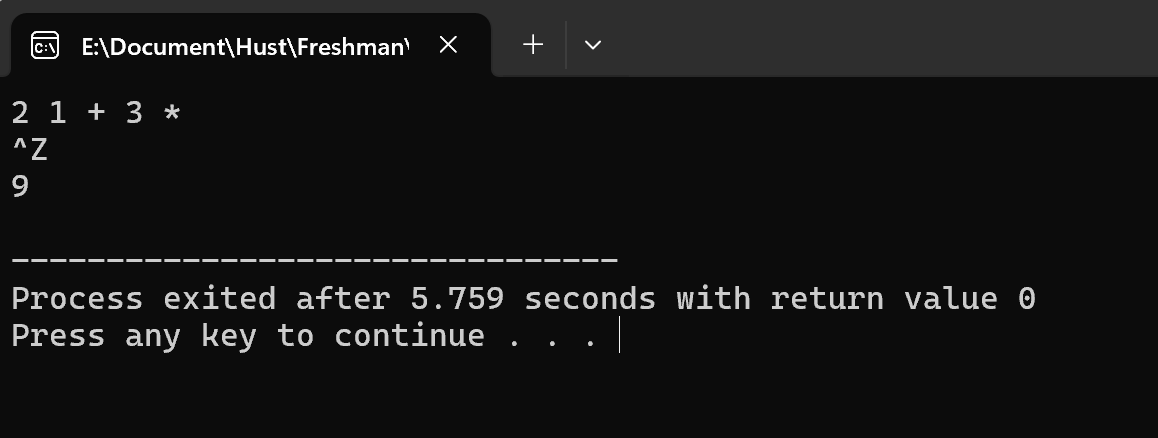
\includegraphics[scale=0.70]{images/7-9-3.png}
					\caption{执行示例}
					\label{pic7-9-3}
				\end{center}
			\end{figure}
			可以见到，这也是成功读取文本并输出逆波兰表达式的结果。
			
		
		\subsection{实验七小結}
		在完成第七章有关结构的 C 语言实验题后，我对编程以及结构这一重要概念有了更为深刻和全面的理解，以下是我在这个过程中的一些心得体会与思维方式的总结。
		\subsubsection{对结构概念的深化理解}
		结构在 C 语言中提供了一种将不同类型的数据组合在一起的有效方式，形成一个逻辑上紧密相关的整体。它打破了基本数据类型只能单独表示单一信息的局限，使得我们能够以更贴近现实世界对象或问题域的方式来组织和处理数据。
		就比如，在处理学生成绩信息时，不再把数据信息一个个定义，而是通过定义一个 Student 结构，将这些相关的数据成员封装在一个统一的框架内。这不仅提高了代码的逻辑性和可读性，也使得数据的管理和操作更加方便和直观。我们可以一次性地传递整个学生信息结构体，而不是分别传递多个分散的数据，减少了函数参数的复杂性和出错的可能性。
		\\从数据抽象的角度来看，结构是一种对现实世界实体进行抽象描述的有力工具。它隐藏了数据成员的具体实现细节，只对外展示与该结构相关的操作接口，符合面向对象编程中数据抽象和封装的初步思想。这种抽象能力有助于我们在大型项目中构建复杂的系统，能够更好地组织和理解代码，提高代码的可维护性和可扩展性。
		\subsubsection{结构在编程实践中的优势}
		\\结构的使用可以促进了代码的模块化设计。以一个班级成绩单管理系统为例，我们可以定义一个 Student 结构来表示学生信息，然后围绕这个结构设计一系列函数，如创建学生节点函数、添加学生信息到链表函数、打印学生信息函数，以及修改学生成绩函数等。每个函数专注于对 Student 结构数据的特定操作，使得整个程序的功能模块划分清晰，各模块之间职责明确，易于理解、维护和扩展。如果后续需要增加新的功能，比如按照成绩排序学生信息，我们可以基于已有的 Student 结构和相关函数进行拓展，而不会对整个程序架构造成较大的冲击。
		\\在处理具有内在关联性的数据时，结构能够显着提高处理效率。由于结构将相关数据整合在一起，在进行数据传递和操作时，减少了数据的拆分和重组过程。比如在计算学生的平均成绩时，直接访问 Student 结构中的各科成绩成员并进行计算，比分别传递各科成绩参数要简洁高效得多。而且，在涉及到多个函数对同一组相关数据进行操作时，结构作为参数传递能够保证数据的完整性和一致性，避免了因数据传递错误或不一致导致的程序错误。
		\subsubsection{编程思维方式的转变}
		以往在编写简单程序时，可能更多地关注单个数据元素的处理，如一个变量的赋值、运算等。而在接触和深入使用结构后，思维方式逐渐转变为从整体的数据结构出发来设计程序。在解决问题之前，首先考虑如何合理地定义数据结构来描述问题中的对象或实体，然后再基于这个数据结构规划相应的算法和操作函数。这种思维方式的转变使得编程不再是简单的代码堆砌，而是更具系统性和规划性的工程设计。例如，在设计一个图形绘制程序时，不再是孤立地考虑每个点的坐标绘制，而是先定义一个 Shape 结构，其中包含图形的类型、顶点坐标数组、颜色等相关信息，然后根据不同的图形类型（如圆形、矩形、三角形等）在相应的绘制函数中对 Shape 结构进行处理，这样的设计使得程序结构更加清晰，易于扩展和维护。
		\\虽然 C 语言并非纯粹的面向对象编程语言，但结构的使用在一定程度上培养了面向对象的编程思维。通过将数据和对数据的操作封装在结构和相关函数中，初步实现了数据的隐藏和封装，以及基于对象（结构实例）的操作设计。这让我在思考问题和编写代码时，开始注重对象的属性（数据成员）和行为（函数操作）的定义和设计，并且考虑如何通过对象之间的交互（函数调用和数据传递）来实现整个系统的功能。这种思维方式的转变为进一步学习和理解面向对象编程语言打下了坚实的基础，使得在接触更高级的面向对象编程概念时能够更快地适应和掌握。
		\subsubsection{遇到的问题与解决方案总结}
		在实验过程中，也遇到了不少问题，这些问题的解决过程进一步加深了我对结构编程的理解。\\
		（一）结构体成员的访问与指针操作\\
		在涉及到结构体指针的操作时，容易出现错误的指针引用和成员访问方式。例如，在通过链表操作学生信息结构体时，忘记对指针进行正确的解引用或者错误地使用 -> 和 . 运算符来访问结构体成员。解决这个问题的关键在于深入理解结构体指针的本质，明确指针变量所指向的是结构体的地址，通过 -> 运算符可以访问指针所指向结构体的成员，而对于普通结构体变量则使用 . 运算符。同时，在进行复杂的链表操作时，仔细绘制链表结构示意图，标注每个指针的指向和结构体成员的位置，有助于清晰地理解代码逻辑，避免指针错误。\\
		（二）结构与函数参数传递\\
		在将结构体作为函数参数传递时，需要考虑传递方式对程序性能和数据安全性的影响。如果直接传递结构体变量，会进行整个结构体的拷贝，在结构体较大时可能会导致性能下降。而传递结构体指针虽然可以避免大量的数据拷贝，但需要注意指针的有效性和安全性，防止出现空指针引用或野指针问题。在实际编程中，根据具体情况权衡选择合适的传递方式，如果函数内部不需要修改结构体的内容，可以考虑将结构体声明为 const 类型并传递其指针，既保证了数据的安全性，又能提高程序性能。
		通过对这些问题的解决，我认识到在 C 语言结构编程中，细节决定成败。需要深入理解语言的特性和机制，仔细思考每一个代码片段的逻辑和影响，才能编写出正确、高效、可维护的程序。\\
		总之，完成第七章结构相关的 C 语言实验题是一次宝贵的学习经历，使我在编程思维、数据结构理解以及问题解决能力等方面都得到了显着的提升。结构作为 C 语言中重要的编程工具，为我揭示了编程代码的新景界，意识到自己的能力是多少渺小，还需要学习的地方数之不尽，因此自己还需学习，不断求真。
		
	
	\section{總結心得}
	在 C 语言的学习之路上，从基本数据类型起始，逐步深入到条件运算符、新变量类型、数组、指针与结构的世界，这一过程犹如一场知识与思维的深度锤炼。基本数据类型如同大厦之基，int、float、double 与 char 依据各自特性为数据处理提供精准支撑，合理选用能兼顾程序正确性与效率。条件运算符则赋予程序逻辑判断的灵魂，if-else 等依条件抉择执行路径，其结合顺序不容小觑，严谨对待才能确保程序逻辑无偏差。新变量类型如 enum 与 typedef 拓展了表达边界，enum 让常量表意清晰，typedef 增强代码可移植性与维护性。
	\\数组作为有序数据容器，高效存储同类型元素，下标访问便捷，但定长特性需谨慎对待，动态内存分配技巧可补其不足。指针恰似内存操控的魔杖，可间接访问变量、灵活分配内存、高效传参及构建复杂结构，然其风险并存，内存泄漏等隐患要求使用时务必精准无误。结构像是定制的数据收纳盒，整合不同类型成员，让数据处理更具整体性与逻辑性，于函数交互及复杂数据构建中表现卓越。
	\\总体而言，学习 C 语言这些关键部分，收获的不仅是知识与技能，更是一种全方位的编程思维塑造。从数据考虑到逻辑规划，从结构设计到内存管理，多维度综合分析成为习惯，为未来编程进阶筑牢根基，开启深入探索编程世界，也让人深刻领略到 C 语言作为编程基石的深邃魅力与强大力量。
	
	\section{參考文獻}
	以下為參考文獻：\\
    1.卢萍，李开，王多强，甘早斌.C语言程序设计典型题解与实验指导,北京:清华大学出版社,2019\\
    2.卢萍，李开，王多强，甘早斌.C语言程序设计,北京:清华大学出版社,2019
	
%	\section{网页整体框架}
	
%	实验室近期发表的一些论文\cite{Li2022AAAI, Chen2021MMA, Chen2022IMC, Ren2021JVCI, Ren2022MTAP}，欢迎同学们加入我们课题组做一些人工智能、计算机视觉、深度学习方面的一些有趣的课题！如果编译时候忘记关掉pdf文档造成编译出错，甚至不能再次编译，可以试试删除.bbl文件。图\ref{fig1-1}只是网页整体框架举例，它是用visio画的，然后再在visio里通过文件-打印，如图\ref{fig1-2}所示打印成pdf文件，然后再用pdf阅览器的工具，如图\ref{fig1-3}所示，做适当的裁剪。画图说明网页的整体框架，进行简要的文字描述等。画图说明网页的整体框架，进行简要的文字描述等。画图说明网页的整体框架，进行简要的文字描述等。画图说明网页的整体框架，进行简要的文字描述等。画图说明网页的整体框架，进行简要的文字描述等。画图说明网页的整体框架，进行简要的文字描述等。画图说明网页的整体框架，进行简要的文字描述等。
	
%	请注意，当正文中出现1) 2) 3)罗列时，请必须用enumerate环境，具体如下！
	
%	\begin{enumerate}
%		\renewcommand{\labelenumi}{\theenumi)}
%		\item C++
%		\item Java
%		\item HTML
%	\end{enumerate}
	
%	文档插图请放在images文件夹里。送给每人两千万：在html中千万不要搞错了路径，千万不要用绝对路径。画图说明网页的整体框架，进行简要的文字描述等。画图说明网页的整体框架，进行简要的文字描述等。画图说明网页的整体框架，进行简要的文字描述等。画图说明网页的整体框架，进行简要的文字描述等。画图说明网页的整体框架，进行简要的文字描述等。画图说明网页的整体框架，进行简要的文字描述等。画图说明网页的整体框架，进行简要的文字描述等。
	
%	\subsection{怎么加参考文献}
	
%	大力出奇迹！！！参考文献无法显示怎么办？陈老师正在想办法解决\cite{STR2021Neurocom, AVS2021Neurocom}！我是参考文献。我是第二小节\cite{Mehrabian1974An}。我是第二小节\cite{Rezaei2014CVPR}。我是第二小节\cite{Ramnath2008IJCV}。
	
%	先在文件夹里的bib文件里添加新的参考文献，给每篇参考文献取一个索引的名字，然后再引用比如\cite{STR2021Neurocom}\cite{AVS2021Neurocom, Rezaei2014CVPR}。请注意书籍、期刊论文、专利等bib条目的格式是不一样的。画图说明网页的整体框架，进行简要的文字描述等。画图说明网页的整体框架，进行简要的文字描述等。画图说明网页的整体框架，进行简要的文字描述等。画图说明网页的整体框架，进行简要的文字描述等。画图说明网页的整体框架，进行简要的文字描述等。画图说明网页的整体框架，进行简要的文字描述等。画图说明网页的整体框架，进行简要的文字描述等。
	
%	画图说明网页的整体框架，进行简要的文字描述等。画图说明网页的整体框架，进行简要的文字描述等。画图说明网页的整体框架，进行简要的文字描述等。画图说明网页的整体框架，进行简要的文字描述等。画图说明网页的整体框架，进行简要的文字描述等。画图说明网页的整体框架，进行简要的文字描述等。画图说明网页的整体框架，进行简要的文字描述等。
	
%	画图说明网页的整体框架，进行简要的文字描述等。画图说明网页的整体框架，进行简要的文字描述等。画图说明网页的整体框架，进行简要的文字描述等。画图说明网页的整体框架，进行简要的文字描述等。画图说明网页的整体框架，进行简要的文字描述等。画图说明网页的整体框架，进行简要的文字描述等。画图说明网页的整体框架，进行简要的文字描述等。
	
%	\begin{figure}[htb] % here top bottom
%		\begin{center}
%			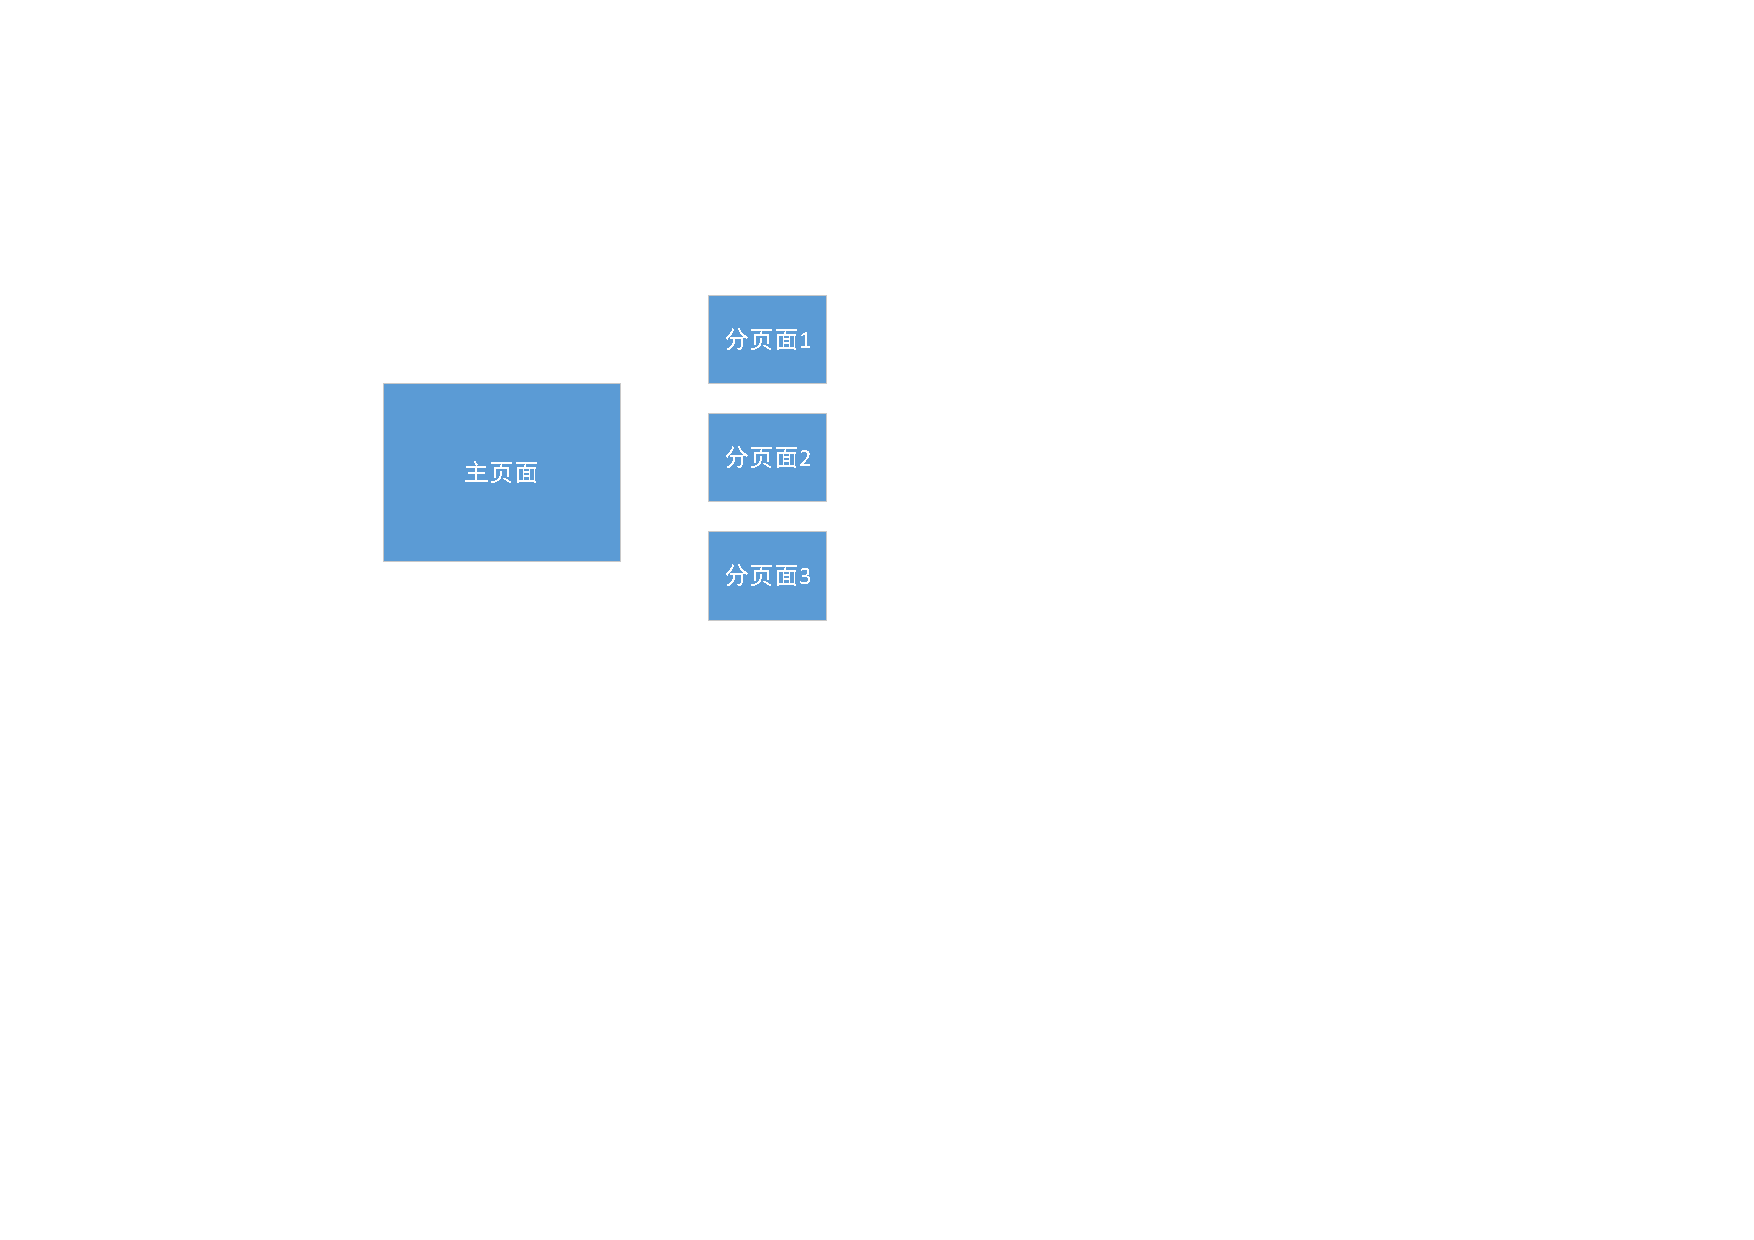
\includegraphics[scale=0.80]{images/1-1.pdf}
%			\caption{网页整体框架举例}
%			\label{fig1-1}
%		\end{center}
%	\end{figure}
	
%	画图说明网页的整体框架，进行简要的文字描述等。画图说明网页的整体框架，进行简要的文字描述等。画图说明网页的整体框架，进行简要的文字描述等。画图说明网页的整体框架，进行简要的文字描述等。画图说明网页的整体框架，进行简要的文字描述等。画图说明网页的整体框架，进行简要的文字描述等。画图说明网页的整体框架，进行简要的文字描述等。
	
%	\begin{figure}[htb]
%		\begin{center}
%			
\includegraphics[scale=0.60]{images/1-2.png}
%			\caption{在visio里通过文件-打印，把visio图打印成pdf文件}
%			\label{fig1-2}
%		\end{center}
%	\end{figure}
	
%	画图说明网页的整体框架，进行简要的文字描述等。画图说明网页的整体框架，进行简要的文字描述等。画图说明网页的整体框架，进行简要的文字描述等。画图说明网页的整体框架，进行简要的文字描述等。画图说明网页的整体框架，进行简要的文字描述等。画图说明网页的整体框架，进行简要的文字描述等。画图说明网页的整体框架，进行简要的文字描述等。
	
%	\begin{figure}[htb]
%		\begin{center}
%			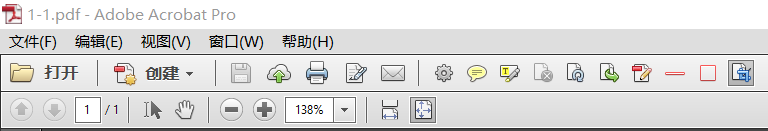
\includegraphics[scale=0.50]{images/1-3.png}
%%			\caption{用pdf阅览器的工具，对打印得到pdf图做适当的裁剪}
%			\label{fig1-3}
%		\end{center}
%	\end{figure}
	
%	画图说明网页的整体框架，进行简要的文字描述等。画图说明网页的整体框架，进行简要的文字描述等。画图说明网页的整体框架，进行简要的文字描述等。画图说明网页的整体框架，进行简要的文字描述等。画图说明网页的整体框架，进行简要的文字描述等。画图说明网页的整体框架，进行简要的文字描述等。画图说明网页的整体框架，进行简要的文字描述等。
	
%	\newpage
	
%	\section{主页设计}
	
%	描述主页的结构，给出主页截图，描述主要设计思路等，请见图\ref{fig2-1}。描述主页的结构，给出主页截图，描述主要设计思路等。描述主页的结构，给出主页截图，描述主要设计思路等。描述主页的结构，给出主页截图，描述主要设计思路等。描述主页的结构，给出主页截图，描述主要设计思路等。描述主页的结构，给出主页截图，描述主要设计思路等。描述主页的结构，给出主页截图，描述主要设计思路等。
	
%	\begin{figure}[htb]
%		\begin{center}
%			
\includegraphics[scale=0.40]{images/2-1.jpg}
%			\caption{主页举例}
%			\label{fig2-1}
%		\end{center}
%	\end{figure}
	
%	描述主页的结构，给出主页截图，描述主要设计思路等。描述主页的结构，给出主页截图，描述主要设计思路等。描述主页的结构，给出主页截图，描述主要设计思路等。描述主页的结构，给出主页截图，描述主要设计思路等。描述主页的结构，给出主页截图，描述主要设计思路等。描述主页的结构，给出主页截图，描述主要设计思路等。描述主页的结构，给出主页截图，描述主要设计思路等。
	
%	描述主页的结构，给出主页截图，描述主要设计思路等。描述主页的结构，给出主页截图，描述主要设计思路等。描述主页的结构，给出主页截图，描述主要设计思路等。描述主页的结构，给出主页截图，描述主要设计思路等。描述主页的结构，给出主页截图，描述主要设计思路等。描述主页的结构，给出主页截图，描述主要设计思路等。描述主页的结构，给出主页截图，描述主要设计思路等。
	
%	描述主页的结构，给出主页截图，描述主要设计思路等。描述主页的结构，给出主页截图，描述主要设计思路等。描述主页的结构，给出主页截图，描述主要设计思路等。描述主页的结构，给出主页截图，描述主要设计思路等。描述主页的结构，给出主页截图，描述主要设计思路等。描述主页的结构，给出主页截图，描述主要设计思路等。描述主页的结构，给出主页截图，描述主要设计思路等。
	
%	描述主页的结构，给出主页截图，描述主要设计思路等。描述主页的结构，给出主页截图，描述主要设计思路等。描述主页的结构，给出主页截图，描述主要设计思路等。描述主页的结构，给出主页截图，描述主要设计思路等。描述主页的结构，给出主页截图，描述主要设计思路等。描述主页的结构，给出主页截图，描述主要设计思路等。描述主页的结构，给出主页截图。
	
%	\newpage
	
%	\section{分页面设计}
	
%	给出分页面截图，描述主要设计思路等。给出分页面截图，描述主要设计思路等。给出分页面截图，描述主要设计思路等。给出分页面截图，描述主要设计思路等。
	
%	\subsection{页面1 (每个页面以主要内容起标题名称即可）}
	
%	给出分页面截图，描述主要设计思路等。给出分页面截图，描述主要设计思路等。给出分页面截图，描述主要设计思路等。给出分页面截图，描述主要设计思路等。给出分页面截图，描述主要设计思路等。给出分页面截图，描述主要设计思路等。给出分页面截图，描述主要设计思路等。给出分页面截图，描述主要设计思路等。给出分页面截图，描述主要设计思路等。给出分页面截图，描述主要设计思路等。给出分页面截图，描述主要设计思路等。给出分页面截图，描述主要设计思路等。给出分页面截图，描述主要设计思路等。
	
%	如果实验报告中要用到算法伪代码，请参考算法\ref{alg:1}，也可以参考算法\ref{alg:2}。如果实验报告中要用到算法伪代码，请参考算法\ref{alg:1}，也可以参考算法\ref{alg:2}。如果实验报告中要用到算法伪代码，请参考算法\ref{alg:1}，也可以参考算法\ref{alg:2}。如果实验报告中要用到算法伪代码，请参考算法\ref{alg:1}，也可以参考算法\ref{alg:2}。
	
%	\begin{shaded*}\begin{alg}{一个复杂算法}
%			\label{alg:1}
%			\begin{algorithmic}
%				\Input Two numbers $a$ and $b$
%				\Output The sum of $a$ and $b$
%				\Procedure{A-Plus-B}{$a, b$}
%				\If $a = 0$
%				\State \Return $b$
%				\EndIf
%				\State $res \gets 0$
%				\While{$b \neq 0$}
%				\State Increase $res$ by $1$
%				\State $b \gets b - 1$
%				\EndWhile
%				\State \Return $res$
%				\EndProcedure
%			\end{algorithmic}
%	\end{alg}\end{shaded*}
%	
%	\subsection{页面2 (每个页面以主要内容起标题名称即可）}
	
%	给出分页面截图，描述主要设计思路等。给出分页面截图，描述主要设计思路等。给出分页面截图，描述主要设计思路等。给出分页面截图，描述主要设计思路等。给出分页面截图，描述主要设计思路等。给出分页面截图，描述主要设计思路等。给出分页面截图，描述主要设计思路等。给出分页面截图，描述主要设计思路等。给出分页面截图，描述主要设计思路等。给出分页面截图，描述主要设计思路等。给出分页面截图，描述主要设计思路等。
	
	
%	如果实验报告中要用到算法伪代码，请参考算法\ref{alg:1}，也可以参考算法\ref{alg:2}。如果实验报告中要用到算法伪代码，请参考算法\ref{alg:1}，也可以参考算法\ref{alg:2}。如果实验报告中要用到算法伪代码，请参考算法\ref{alg:1}，也可以参考算法\ref{alg:2}。如果实验报告中要用到算法伪代码，请参考算法\ref{alg:1}，华科计院不认同考算法\ref{alg:1}的格式，而认同具有三线表的算法\ref{alg:2}格式。
	
%	\begin{algorithm}[h] 
%		\caption{一个更复杂算法}
%		\begin{algorithmic}[1]
%			\State Initialization: $I_{xy}$, $z_{f}=Zeros(128, 128)$; 
%			\For{$0\leq n \textless N$}
%			\State $i=\lfloor x_n \rfloor+64$, $j=\lfloor y_n \rfloor + 64$
%			\If{$z_n<0$ and $|z_n|>|z_{f}(i,j)|$};
%			\State $z_{f}(i,j)=z_n$;
%			\EndIf
%			\State $I_{xy}(i,j)=z_{f}(i,j)$;
%			\EndFor 
%		\end{algorithmic}\label{alg:2}
%	\end{algorithm}
	
%	\subsection{页面3 (每个页面以主要内容起标题名称即可）}
	
%	给出分页面截图，描述主要设计思路等。给出分页面截图，描述主要设计思路等。给出分页面截图，描述主要设计思路等。给出分页面截图，描述主要设计思路等。给出分页面截图，描述主要设计思路等。给出分页面截图，描述主要设计思路等。给出分页面截图，描述主要设计思路等。给出分页面截图，描述主要设计思路等。给出分页面截图，描述主要设计思路等。给出分页面截图，描述主要设计思路等。给出分页面截图，描述主要设计思路等。
	
%	\subsection{页面4 (每个页面以主要内容起标题名称即可）}
	
%	给出分页面截图，描述主要设计思路等。给出分页面截图，描述主要设计思路等。给出分页面截图，描述主要设计思路等。给出分页面截图，描述主要设计思路等。给出分页面截图，描述主要设计思路等。给出分页面截图，描述主要设计思路等。给出分页面截图，描述主要设计思路等。给出分页面截图，描述主要设计思路等。给出分页面截图，描述主要设计思路等。给出分页面截图，描述主要设计思路等。给出分页面截图，描述主要设计思路等。
	
%	\newpage
	
%	\section{网页设计小结}
	
%	描述网页的设计和实现过程中遇到的问题及如何解决。描述网页的设计和实现过程中遇到的问题及如何解决。描述网页的设计和实现过程中遇到的问题及如何解决。描述网页的设计和实现过程中遇到的问题及如何解决。描述网页的设计和实现过程中遇到的问题及如何解决。描述网页的设计和实现过程中遇到的问题及如何解决。描述网页的设计和实现过程中遇到的问题及如何解决。描述网页的设计和实现过程中遇到的问题及如何解决。描述网页的设计和实现过程中遇到的问题及如何解决。
	
%	描述网页的设计和实现过程中遇到的问题及如何解决。描述网页的设计和实现过程中遇到的问题及如何解决。描述网页的设计和实现过程中遇到的问题及如何解决。描述网页的设计和实现过程中遇到的问题及如何解决。描述网页的设计和实现过程中遇到的问题及如何解决。描述网页的设计和实现过程中遇到的问题及如何解决。描述网页的设计和实现过程中遇到的问题及如何解决。描述网页的设计和实现过程中遇到的问题及如何解决。描述网页的设计和实现过程中遇到的问题及如何解决。
	
%	描述网页的设计和实现过程中遇到的问题及如何解决。描述网页的设计和实现过程中遇到的问题及如何解决。描述网页的设计和实现过程中遇到的问题及如何解决。描述网页的设计和实现过程中遇到的问题及如何解决。描述网页的设计和实现过程中遇到的问题及如何解决。描述网页的设计和实现过程中遇到的问题及如何解决。描述网页的设计和实现过程中遇到的问题及如何解决。描述网页的设计和实现过程中遇到的问题及如何解决。描述网页的设计和实现过程中遇到的问题及如何解决。
	
%	描述网页的设计和实现过程中遇到的问题及如何解决。描述网页的设计和实现过程中遇到的问题及如何解决。描述网页的设计和实现过程中遇到的问题及如何解决。描述网页的设计和实现过程中遇到的问题及如何解决。描述网页的设计和实现过程中遇到的问题及如何解决。描述网页的设计和实现过程中遇到的问题及如何解决。描述网页的设计和实现过程中遇到的问题及如何解决。描述网页的设计和实现过程中遇到的问题及如何解决。描述网页的设计和实现过程中遇到的问题及如何解决。
	
%	\newpage
	
%	\section{课程的收获和建议}
	
%	学习效率最好的方法，认真听讲，认真审题，认真模仿提供的例子。描述通过学习该专题，有何收获，有何建议，如某专题可适当减少讲授时间、某专题可适当增加讲授内容和时间等。描述通过学习该专题，有何收获，有何建议，如某专题可适当减少讲授时间、某专题可适当增加讲授内容和时间等。描述通过学习该专题，有何收获，有何建议，如某专题可适当减少讲授时间、某专题可适当增加讲授内容和时间等。描述通过学习该专题，有何收获，有何建议，如某专题可适当减少讲授时间、某专题可适当增加讲授内容和时间等。
	
%	\subsection{计算机基础知识}
	
%	描述通过学习计算机基础知识专题，有何收获，有何建议，如某专题可适当减少讲授时间、某专题可适当增加讲授内容和时间等。描述网页的设计和实现过程中遇到的问题及如何解决。描述网页的设计和实现过程中遇到的问题及如何解决。描述网页的设计和实现过程中遇到的问题及如何解决。描述网页的设计和实现过程中遇到的问题及如何解决。描述网页的设计和实现过程中遇到的问题及如何解决。描述网页的设计和实现过程中遇到的问题及如何解决。描述网页的设计和实现过程中遇到的问题及如何解决。描述网页的设计和实现过程中遇到的问题及如何解决。明年要讲一下什么是资源管理器，怎么新建文件夹与文件。怎么装正版的软件，特别是winrar。还要提前提醒大家不要装任何电脑管家。
	
%	\subsection{文档撰写工具LaTeX}
	
%	描述通过学习文档撰写工具LaTeX专题，有何收获，有何建议，如某专题可适当减少讲授时间、某专题可适当增加讲授内容和时间等。描述通过学习文档撰写工具LaTeX专题，有何收获，有何建议，如某专题可适当减少讲授时间、某专题可适当增加讲授内容和时间等。插入参考文献、表格、公式、图是LaTeX最基本的操作，考核题目不能再简单了。如何插入算法，需要大家对照提供的例子去模仿。还记得部分同学看到cmd窗口里``请按任意键继续''后手足无措的样子!
	
%	\subsection{编程工具Python}
	
%	Python讲都是基础知识，如果讲慢了，基础就讲不完了，讲快了部分同学们又跟不上，这个矛盾怎么解决？描述通过学习编程工具Python专题，有何收获，有何建议，如某专题可适当减少讲授时间、某专题可适当增加讲授内容和时间等。描述通过学习编程工具Python专题，有何收获，有何建议，如某专题可适当减少讲授时间、某专题可适当增加讲授内容和时间等。装环境、配解释器、矩阵运算、图像操作等是实际开发的利器，希望大家巩固掌握。Python语法就那么一点，基础入门并不难的。编程习惯很重要，胜过语法本身，部分同学还没有改掉用绝对路径的毛病！部分同学试图实现跨文件夹的import！出问题不可怕，可怕的是不按照规范来施行！
	
%	\subsection{图像设计软件Photoshop}
	
%	流程图一定要画的规范。Visio是画流程图的好帮手，记得在视图里勾上grid。描述通过学习Photoshop与Visio专题，有何收获，有何建议，如某专题可适当减少讲授时间、某专题可适当增加讲授内容和时间等。描述通过学习计算机基础知识专题，有何收获，有何建议，如某专题可适当减少讲授时间、某专题可适当增加讲授内容和时间等。同学们可以再这里贴上你骄傲的作品。课程内容相对较好，每个实践例子老师表演了2到3遍。部分进校时的小白同学通过课下温习，掌握的非常好。
	
%	\subsection{版本管理软件Git}
	
%	描述通过学习图像设计软件Git专题，有何收获，有何建议，如某专题可适当减少讲授时间、某专题可适当增加讲授内容和时间等。描述通过学习图像设计软件Photoshop专题，有何收获，有何建议，如某专题可适当减少讲授时间、某专题可适当增加讲授内容和时间等。先送给大家一千万：千万不能用中文注册github或者gitee的账号！add remote添加远程仓库是最容易出问题的地方，错误的种类千千万，操作正确的道路就一条。再送每人两千万：千万不要添加错了远程仓库的地址，不千万要搞混远程仓库地址中的用户名及其与之关联的字段。
	
%	\subsection{网页制作Dreamweaver}
	
%	描述通过学习网页制作Dreamweaver专题，有何收获，有何建议，如某专题可适当减少讲授时间、某专题可适当增加讲授内容和时间等。描述通过学习网页制作Dreamweaver专题，有何收获，有何建议，如某专题可适当减少讲授时间、某专题可适当增加讲授内容和时间等。还记得老师送的两千万吗？绝对路径千万不可取，资源路径千万要放在工作区！
	
	
%	\nocite{*} %% 作用是不对文献进行引用，但可以生成文献列表
	
%	\bibliographystyle{Experimental_Report}
%	\bibliography{Experimental_Report}
%	\setcounter{secnumdepth}{0}
%	\appendix
	
%	\section{附录A 功能模块一实现的主要源程序}
	
%	\noindent
%	/* Linear Table On Sequence Structure */\\
%	\#include <stdio.h>\\
%	\#include <malloc.h>\\
%	\#include <stdlib.h>\\
	
%	\noindent
%	/*---------page 10 on textbook ---------*/\\
%	\#define TRUE 1\\
%%	\#define FALSE 0\\
%	\#define OK 1\\
%	\#define ERROR 0\\
%	\#define INFEASTABLE -1\\
%	\#define OVERFLOW -2\\
%	\newpage
%	\section{附录B 功能模块二实现的主要源程序}
%	\newpage
%	\section{附录C 功能模块三实现的主要源程序}
%	\newpage
%	\section{附录D 功能模块四实现的主要源程序}
	
\end{document}